\documentclass[a4paper]{article}

\usepackage{NotesPackage2}
\usepackage{subcaption}
\usepackage[version=4]{mhchem}
\usepackage{hyperref}

\usetikzlibrary{calc}
\usetikzlibrary{decorations.markings}

\author{Willoughby Seago}
\date{September 22, 2020}
\title{Electromagnetism}

% particles
\newcommand{\downQuark}{\mathrm{d}}
\newcommand{\electron}{{\mathrm{e}^-}}
\newcommand{\proton}{\mathrm{p}}
\newcommand{\anti}[1]{\bar{#1}}

% Letters for specific things where a weird font is needed
\newcommand{\region}{\mathcal{R}}
\newcommand{\boundary}{\mathcal{B}}
\newcommand{\quadrupole}{\mathcal{Q}}
\newcommand{\current}{\mathcal{I}}
\newcommand{\emf}{\mathcal{E}}

% units
\DeclareSIUnit{\gauss}{G}
\DeclareSIUnit{\gaussAlternate}{Gs}

% other
\newcommand{\notesVersion}{1.0}
\newcommand{\notesDate}{23/12/2020}
\newcommand{\vhsub}[2]{\vh{#1}\bm{#2}}
\DeclareMathOperator{\sgn}{sgn}
\newcommand{\enc}{{\mathrm{enc}}}

\makeglossaries
% Add glossary entries here
\newacronym{em}{EM}{electromagnetism}
\newacronym{pde}{PDE}{partial differential equation}
\newacronym{bc}{BC}{boundary conditions}
\newacronym{pe}{PE}{Poisson's equation}
\newacronym{le}{LE}{Laplace's equation}
\newacronym{emf}{emf}{electromotive force}
\newacronym{lih}{LIH}{linear isotropic homogeneous}

\includeonly{parts/electrostatics, parts/magnetostatics, parts/electromagnetism}

\begin{document}
    \pagenumbering{roman}  % Number contents pages and glossaries with roman numerals
    \maketitle
    These are my notes for the \textit{electromagnetism} course from the University of Edinburgh as part of the third year of the theoretical physics degree.
    When I took this course in the 2020/21 academic year it was taught by Dr Andreas Hermann\footnote{\url{https://www.ph.ed.ac.uk/people/andreas-hermann}} and Dr Jamie Cole\footnote{\url{https://www.ph.ed.ac.uk/people/jamie-cole}}.
    These notes are based on the lectures delivered as part of this course, the notes provided as part of this course, and the book `introduction to electrodynamics'\footnote{Griffiths, D.~J. \textit{Introduction to Electrodynamics}, fourth edition (Cambridge University Press, Cambridge, 2017)}.
    The content within is correct to the best of my knowledge but if you find a mistake or just disagree with something or think it could be improved please let me know.
    
    These notes were produced using \LaTeX\footnote{\url{https://www.latex-project.org/}}.
    Graphs where plotted using Matplotlib\footnote{\url{https://matplotlib.org/}}, NumPy\footnote{\url{https://numpy.org/}}, and SciPy\footnote{\url{https://scipy.org/scipylib/}}.
    Diagrams were drawn with tikz\footnote{\url{https://www.ctan.org/pkg/pgf}}.
    
    This is version \notesVersion~of these notes, which is up to date as of \notesDate.
    \begin{flushright}
        Willoughby Seago
        
        s1824487@ed.ac.uk
    \end{flushright}
    \clearpage
    \tableofcontents
    \listoffigures
    \printglossary[type=\acronymtype, title=Acronyms, style=long]
    \clearpage
    \pagenumbering{arabic}  % Number rest of document with numbers
    \begingroup
    \let\clearpage\relax  % "\begingroup, \let\clearpage\relax, \endgroup" stops automatic pagebreaks after each include
        \section{Vector Calculus}
    \subsection{Gradient}
    The \define{gradient} of a scalar field, \(f\colon\reals^n\to\reals\), is a function, \(\grad f\colon\reals^n\to\reals^n\), defined in three dimensions, in Cartesian coordinates, \((x, y, z)\), by
    \[\operatorname{grad}f = \grad f =  \pdv{f}{x}\ve x + \pdv{f}{y}\ve y + \pdv{f}{z}\ve z = \partial_i f\ve{i}\]
    with the Einstein summation convention applied in the last term.
    The gradient of a function can be thought of as a vector operator, \(\grad\), acting on a scalar field, \(f\), to give a vector field, \(\grad f\).
    This vector field points in the direction of maximum increase of \(f\) and its magnitude is a measure of how fast \(f\) increases in this direction.
    Because of this the gradient is perpendicular to the level surfaces as travelling along a level surface means that by definition \(f\) is constant.
    
    One important gradient to remember is
    \[\grad r = \vh{r}\]
    where, \(\vh{r}\), represents a unit vector in the direction of \(\vv{r}\).
    Another important fact is that
    \[\int_A^B \grad f \cdot\,\dd\vv{l} = f(\vv{r}_B) - f(\vv{r}_A)\]
    where \(\vv{r}_A\) and \(\vv{r}_B\) are the points \(A\) and \(B\) respectively.
    This is independent of the path taken from \(A\) to \(B\) as \(\grad f\) is always a conservative field, we will see this again later.
    
    The gradient looks different in different coordinates.
    In cylindrical coordinates, \((\rho, \varphi, z)\), it is
    \[\grad f = \pdv{t}{\rho}\ve{\rho} + \frac{1}{\rho}\pdv{f}{\varphi}\ve{\varphi} + \pdv{f}{z}\ve{z},\]
    and in spherical coordinates, \((r, \vartheta, \varphi)\),\footnote{We use the physics convention of \(\vartheta\) as the polar angle from the \(z\)-axis and \(\varphi\) as the azimuthal angle from the \(x\)-axis.} it is
    \[\grad f = \pdv{f}\ve{r} + \frac{1}{r}\pdv{f}{\vartheta}\vh{\vartheta} + \frac{1}{r\sin\vartheta}\pdv{f}{\varphi}\ve{\varphi}.\]
    Importantly if \(f = f(r)\) (i.e. there is no dependence on \(\vartheta\) or \(\varphi\)) then
    \[\grad f = \pdv{f}{r}\ve{r}.\]
    This is consistent with the chain rule which is
    \[\grad f(r) = \dv{f}{r}\grad{r} = \dv{f}{r}\vh{r} = \dv{f}{r}\ve{r}.\]
    Here \(f\) is a function of one variable so partial and total derivatives are equivalent.
    An important example of this chain rule is
    \[\grad\frac{1}{r} = -\frac{1}{r^2}\vh{r} = -\frac{1}{r^3}\vv{r}.\]
    
    \subsection{Divergence and Gauss' Theorem}
    \subsubsection{Divergence}
    The \define{divergence} of a vector field, \(\vv{K}\colon\reals^n\to\reals^n\), is a function, \(\div\vv{K}\colon\reals^n\to\reals\), defined in three dimensions, in Cartesian coordinates, \((x, y, z)\), by
    \[\operatorname{div}f = \div f = \pdv{K_x}{x} + \pdv{K_y}{y} + \pdv{K_z}{z} = \partial_i K_i.\]
    The divergence of a function can be thought of as the scalar product of a vector operator, \(\grad\), and a vector field, \(\vv{K}\), to give a scalar field, \(\div\vv{K}\).
    The divergence gives a measure of how fast the flux lines of the vector field \(\vv{K}\) converge towards a sink \((\div\vv{K} < 0)\) or diverge away from a source \((\div\vv{K}) > 0\).
    
    One important divergence to remember is
    \[\div\vv r = \pdv{x}{x} + \pdv{y}{y} + \pdv{z}{z} = 3.\]
    The divergence looks different in different coordinates.
    In cylindrical coordinates, \((\rho, \varphi, z)\), it is
    \[\div\vv{K} = \frac{1}{\rho}\pdv{\rho}(\rho K_\rho) + \frac{1}{\rho}\pdv{K_\varphi}{\varphi} + \pdv{K_z}{z},\]
    and in spherical coordinates, \((r, \vartheta, \varphi)\), it is
    \[\div\vv{K} = \frac{1}{r^2}\pdv{r}(r^2K_r) + \frac{1}{r\sin\vartheta}\pdv{\vartheta}(K_\vartheta\sin\vartheta) + \frac{1}{r\sin\vartheta}\\pdv{K_\varphi}{\varphi}.\]
    
    \subsubsection{Gauss' Theorem}
    \define{Gauss' theorem},\footnote{Not to be confused with the similar Gauss' law, see section~\ref{sec:Gauss' law}} also known as the \define{divergence theorem}, is
    \[\int_V\div\vv{K}\,\dd V = \oint_A\vv K\cdot\dd\vv{S}\]
    where \(A\) is a closed surface enclosing the volume \(V\), \(\dd{V} = \dd{x}\dd{y}\dd{z} = \dd[3]{r}\) is a volume element, \(\dd{\vv{S}} = \vh{n}\dd{S}\) is a surface element pointing out of the volume, and \(\vv K\) is a vector field.
    Gauss' theorem holds for any such closed surface, \(A\), and the volume it defines and any vector field, \(\vv K\).
    This theorem relates a surface integral over a closed surface to an integral of the volume enclosed.
    This is very useful if we don't care about the nature of the field inside the volume and we only want to know its integral over that volume as it much easier to perform a surface integral.
    
    \subsection{Curl and Stokes' Theorem}
    \subsubsection{Curl}
    The \define{curl} of a vector field, \(\vv{K}\colon\reals^3\to\reals^3\), is a function \(\curl\vv{K}\colon\reals^3\to\reals^3\), defined in Cartesian coordinates, \((x, y, z)\), by
    \begin{align*}
        \operatorname{curl}\vv{K} = \curl \vv{K} &= \left(\pdv{K_z}{y} - \pdv{K_y}{z}\right)\ve{x} + \left(\pdv{K_x}{z} - \pdv{K_z}{x}\right)\ve{y} + \left(\pdv{K_y}{x} - \pdv{K_x}{y}\right)\\
        &=
        \begin{vmatrix}
            \ve{x} & \ve{y} & \ve{z}\\
            \partial_x & \partial_y & \partial_z\\
            K_x & K_y & K_z
        \end{vmatrix}
        \\
        &= \varepsilon_{ijk}\partial_i K_j\ve{k}
    \end{align*}
    where \(\varepsilon_{ijk}\) is the Levi-Civita symbol.
    The curl looks different in different coordinates.
    In cylindrical coordinates, \((\rho, \varphi, z)\), it is
    \[\curl\vv{K} = \left(\frac{1}{\rho}\pdv{K_z}{\varphi} - \pdv{K_\varphi}{z}\right)\ve{\rho} + \left(\pdv{K_\rho}{z} - \pdv{K_z}{\rho}\right)\ve{\varphi} + \frac{1}{\rho}\left(\pdv{\rho}(\rho K_\varphi) - \pdv{K_\rho}{\varphi}\right)\ve{z},\]
    and in spherical coordinates, \((r, \vartheta, \varphi)\), it is
    \begin{align*}
        \curl\vv{K} &= \frac{1}{r\sin\vartheta}\left(\pdv{\vartheta}(K_\varphi\sin\vartheta) - \pdv{K_\vartheta}{\varphi}\right)\ve{r}\\
        &\qquad+ \frac{1}{r}\left(\frac{1}{\sin\vartheta}\pdv{K_r}{\varphi} - \pdv{r}(rK_\varphi)\right)\ve{\vartheta} \\
        &\qquad+ \frac{1}{r}\left(\pdv{r}(rK_\vartheta) - \pdv{K_r}{\vartheta}\right)\ve{\varphi}.
    \end{align*}
    
    \subsubsection{Stokes' Theorem}
    \define{Stokes' theorem} is
    \[\int_A (\curl\vv{K})\cdot\dd\vv{S} = \oint_C\vv{K}\cdot\dd\vv{l}\]
    where \(C\) is a closed curve bounding the surface \(A\), \(\dd\vv{S} = \vh{n}\dd S\) is a surface element, \(\dd\vv{l}\) is a line element that is related to \(\dd\vv{S}\) by the right hand rule, and \(\vv{K}\) is a vector field.
    Stokes' theorem holds for all closed curves, \(C\), and any surface that it defines, as well as any vector field, \(\vv{K}\).
    This theorem relates a line integral over a closed curve to the integral of a surface defined by the curve.
    This is very useful if we don't care about the nature of the field inside the surface and we only want to know its integral over that area as it much easier to perform a line integral.
    
    \subsection{Examples of Non-Vanishing Divergence and Curl}
    \subsubsection{Non-Vanishing Divergence}
    The divergence is non-vanishing if the vector field grows along the propagation direction.
    Consider the vector field drawn in figure~\ref{fig:non-vanishing divergence}.
    \begin{figure}[ht]
        \centering
        \begin{tikzpicture}
            \foreach \y in {0, 1, 2} {
                \draw[->] (0, \y) -- (1, \y);
                \draw[->] (3, \y) -- (5, \y);
                \draw[->] (6, \y) -- (9, \y);
            }
            \draw[dashed] (0.5, -0.5) rectangle (8.5, 2.5);
            \node at (4.5, 3) {\(\vv{K}\cdot\dd\vv{S} = 0\)};
            \node at (4.5, -1) {\(\vv{K}\cdot\dd\vv{S} = 0\)};
            \node[left, text width=2cm, align=center] at (0, 1) {\(\vv{K}\cdot\dd\vv{S}\) small,\\ negative};
            \node[right, text width=2cm, align=center] at (9, 1) {\(\vv{K}\cdot\dd\vv{S}\) large,\\ positive};
        \end{tikzpicture}
        \caption{A vector field, \(\vv{K}\), with non-vanishing divergence.}
        \label{fig:non-vanishing divergence}
    \end{figure}
    We can apply Gauss' theorem to the dashed box.
    Along the top and bottom the surface is parallel to the vector field so the surface normal is perpendicular to the vector field.
    This means that \(\vv K\cdot\dd\vv{S} = 0\).
    On the right hand side \(\vv{K}\) is large and in the same direction as \(\dd\vv{S}\) so \(\vv{K}\cdot\dd\vv{S}\) is positive and large.
    On the left hand side \(\vv{K}\) is small and in the opposite direction to \(\dd\vv{S}\) so \(\vv{K}\cdot\dd\vv{S}\) is negative and small in magnitude.
    The result is that after integrating over the whole surface the left hand side fails to cancel the right hand side and the result is positive.
    Therefore we have
    \[\oint_S\vv{K}\cdot\dd\vv{S} > 0.\]
    This is true for all surfaces, \(S\), that we can draw, specifically it is true if we take \(S\) to be arbitrarily small.
    Using Gauss' theorem this gives us
    \[\int_V\div\vv{K} \dd{V} > 0.\]
    Since this holds for all surfaces, \(S\), it must hold for all volumes, \(V\), so we must have
    \[\div\vv{K} > 0,\]
    meaning the divergence is non-vanishing.
    
    \subsubsection{Non-Vanishing Curl}
    The curl is non-vanishing if the vector field grows perpendicular to the propagation direction.
    Consider the vector field drawn in figure~\ref{fig:non-vanishing curl}.
    \begin{figure}[ht]
        \centering
        \begin{tikzpicture}
            \foreach \x in {0, 4, 8} {
                \foreach \y in {0, 1, 2} {
                    \draw[->] (\x, \y) -- (3 - \y + \x, \y);
                }
            }
            \draw[dashed] (0.5, -0.5) rectangle (8.5, 2.5);
            \draw[->] (4.5, 2.5) -- (4, 2.5) node[below] at (4, 2.5) {\(\dd\vv{l}\)};
            \draw[->] (4.5, -0.5) -- (5, -0.5) node[above] (5, 2.5) {\(\dd\vv{l}\)};
            \node[left] at (0, 1) {\(\vv{K}\cdot\dd\vv{l} = 0\)};
            \node[right] at (11, 1) {\(\vv{K}\cdot\dd\vv{l} = 0\)};
            \node[above] at (4.5, 3) {\(\vv{K}\cdot\dd\vv{l}\) small, negative};
            \node[below] at (4.5, -1) {\(\vv{K}\cdot\dd\vv{l}\) large, positive};
        \end{tikzpicture}
        \caption{A vector field, \(\vv{K}\), with non-vanishing curl.}
        \label{fig:non-vanishing curl}
    \end{figure}
    We can apply Stokes' theorem to the dashed box.
    Along the left and right hand side the curve is perpendicular to the vector field.
    This means that \(\vv{K}\cdot\dd\vv{l} = 0\).
    On the bottom \(\vv{K}\) is large and in the same direction as \(\dd\vv{l}\) so \(\vv{K}\cdot\dd\vv{l}\) is positive and large.
    On the top \(\vv{K}\) is small and in the opposite direction to \(\dd\vv{l}\) so \(\vv{K}\cdot\dd\vv{l}\) is negative and small in magnitude.
    The result is that after integrating over the whole curve the top fails to cancel the bottom and the result is positive.
    Therefore we have
    \[\oint_C \vv{K}\cdot\dd\vv{l} > 0.\]
    This is true for all curves, \(C\), that we can draw, specifically it is true if we take \(C\) to be arbitrarily small.
    Using Stokes' theorem this gives us
    \[\int_A(\curl\vv{K})\cdot\dd\vv{S} > 0.\]
    Since this holds for all curves, \(C\), it must also hold for all surfaces, \(A\), so we must have
    \[\curl\vv{K} > 0,\]
    meaning the curl is non-vanishing.
    
    \subsection{Laplacian}
    The \define{Laplacian} of a scalar field, \(f\colon\reals^n\to\reals\), is a function, \(\laplacian f\colon\reals^n\to\reals\), defined in three dimensions, in Cartesian coordinates, \((x, y, z)\), by
    \[\laplacian f = \div(\grad f) = \pdv[2]{f}{x} + \pdv[2]{f}{y} + \pdv[2]{f}{x} = \partial_i\partial_i f.\]
    The gradient of a scalar function can be thought of as a scalar operator, \(\laplacian = \div\grad\), acting on a scalar field, \(f\), to give a scalar field, \(\laplacian f\).
    The Laplacian is a measure of the curvature of a field, in the same way that the second derivative of \(f\colon\reals\to\reals\) gives a measure of curvature (i.e. it is zero if and only if \(f\) describes a straight line).
    
    Being a scalar operator the Laplacian can also be applied to a vector field, \(\vv{K}\colon\reals^n\to\reals^n\) in which case the Laplacian is a function, \(\laplacian\vv{K}\colon\reals^n\to\reals^n\), defined in three dimensions, in Cartesian coordinates, \((x, y, z)\), by:
    \[\laplacian\vv{K} = \laplacian K_x\ve{x} + \laplacian K_y\ve{y} + \laplacian K_z\ve{z} = \laplacian K_i\ve{i},\]
    where the Laplacians after the first equals are as defined above acting on a scalar field.
    The Laplacian looks different in different coordinates.
    In cylindrical coordinates, \((\rho, \varphi, z)\), it is
    \[\laplacian f = \frac{1}{\rho}\pdv{\rho}\left(\rho\pdv{f}{\rho}\right) + \frac{1}{\rho^2}\pdv[2]{f}{\varphi} + \pdv[2]{f}{z}.\]
    In Spherical coordinates, \((r, \vartheta, \varphi)\), it is
    \begin{align*}
        \laplacian f &= \frac{1}{r^2}\pdv{r}\left(r^2\pdv{f}{r}\right) + \frac{1}{r^2\sin\vartheta}\pdv{\vartheta}\left(\sin\vartheta \pdv{f}{\vartheta}\right) + \frac{1}{r^2\sin^2\vartheta}\pdv[2]{f}{\varphi}\\
        &= \frac{1}{r}\pdv[2]{r}(rf) + \frac{1}{r^2\sin\vartheta}\pdv{\vartheta}\left(\sin\vartheta \pdv{f}{\vartheta}\right) + \frac{1}{r^2\sin^2\vartheta}\pdv[2]{f}{\varphi}
    \end{align*}

    \subsection{Useful Vector Identities}\label{sec:useful vector identities}
    Let \(\varphi, \psi\colon\reals^3\to\reals\), and \(\vv{A}, \vv{B}\colon\reals^3\to\reals^3\) then
    \begin{enumerate}
        \item \(\grad(\varphi\psi) = \varphi\grad\psi + (\grad\varphi)\psi\)
        \item \(\div(\varphi\vv{A}) = \varphi\div\vv{A} + (\grad\varphi)\cdot\vv{A}\)
        \item \(\curl(\varphi\vv{A}) = \varphi(\curl\vv{A}) + (\grad\varphi)\times\vv{A}\)
        \item \(\grad(\vv{A}\cdot\vv{B}) = (\vv{A}\cdot\grad)\vv{B} + (\vv{B}\cdot\grad)\vv{A} + \vv{A}\times(\curl\vv{B}) + \vv{B}\times(\curl\vv{A})\)
        \item \(\div(\vv{A}\times\vv{B}) = \vv{B}\cdot(\curl\vv{A}) - \vv{A}\cdot(\curl\vv{B})\)
        \item \(\curl(\vv{A}\times\vv{B}) = \vv{A}(\div\vv{B}) - \vv{B}(\div\vv{A}) + (\vv{B}\cdot\grad)\vv{A} - (\vv{A}\cdot\grad)\vv{B}\)
        \item \(\curl(\grad f) = 0\)
        \item \(\div(\curl\vv{A}) = 0\)
        \item \(\curl(\curl\vv{A}) = \grad(\div\vv{A}) - \laplacian\vv{A}\)
    \end{enumerate}
    
    \subsection{Taylor Expansions in 3 Dimensions}
    Let \(f\colon\reals^n\to\reals\).
    A small change, \(\dd{\vv{r}}\), in \(\vv{r}\) causes a change \(\dd{f} = \grad f\cdot\dd{\vv{r}}\) in \(f\).
    This is the first term of a 3-dimensional Taylor expansion of \(f\) about the point \(\vv{r'}\):
    \begin{align*}
        f(\vv{r}) &= \sum_{n=0}^\infty \frac{1}{n!}[(\vv{r} - \vv{r'})\cdot\grad]^n f(\vv{r})|_{\vv{r} = \vv{r'}}\\
        &= f(\vv{r'}) + \sum_{i=1}^3(x_i - x'_i)\pdvat{f(\vv{r})}{x_i}{\vv{r} = \vv{r'}} + \frac{1}{2}\sum_{i=1}^3\sum_{j=1}^3(x_i - x'_i)(x_j - x'_j)\pdvsecat{f(\vv{r})}{x_j}{x_i}{\vv{r} = \vv{r'}} + \dotsb
    \end{align*}
    
    \subsection{An Important Theorem}\label{sec:an important theorem}
    The following three statements concerning a vector field, \(\vv{F}\colon V\subseteq\reals^3\to\reals^3\), over some region in space, \(V\), are equivalent:
    \begin{enumerate}
        \item \(\curl\vv{F} = 0\) -- The vector field, \(\vv{F}\), is irrotational.
        \item \(\vv{F} = \grad\varphi\) for some \(\varphi\colon\reals^3\to\reals\) -- The vector field, \(\vv{F}\), is a gradient field of a scalar potential, \(\varphi\).
        \item The line integral
        \[\int_A^B \vv{F}\cdot\dd{\vv{l}}\]
        is independent of the path from \(A\) to \(B\) for all \(A, B\in V\).
        A consequence of this is that for any closed curve, \(C\), in \(V\) we have
        \[\oint_C\vv{F}\cdot\dd{\vv{l}} = 0.\]
    \end{enumerate}
    
    \subsection{The Dirac Delta Distribution}\label{sec:Dirac delta distribution}
    The \define{Dirac Delta distribution} is a generalised function, \(\delta\), with two defining properties:
    \[
        \delta(x - x_0) = 
        \begin{cases}
            0, & x \ne x_0,\\
            \infty, & x = x_0,
        \end{cases}
    \]
    and
    \[\int_{-\infty}^{\infty} \delta(x - x_0)\,\dd{x} = 1.\]
    We can actually be more specific with this last property:
    \[\int_{a}^{b} \delta(x - x_0)\,\dd{x} = 1\]
    if and only if \(x_0\in [a, b]\).
    
    We can define an analogous distribution in 3 dimensions.
    We use the same symbol, \(\delta\), and it has the expected analogous properties:
    \[
        \delta(\vv{r} - \vv{r_0}) = 
        \begin{cases}
            0, & \vv{r} \ne \vv{r_0},\\
            \infty, & \vv{r} = \vv{r_0},
        \end{cases}
    \]
    and
    \[\int_{\reals^3} \delta(\vv{r} - \vv{r_0})\,\dd{V} = 1\]
    or more specifically for some volume \(V\subseteq\reals^3\)
    \[\int_V \delta(\vv{r} - \vv{r_0})\,\dd{V} = 1\]
    if and only if \(\vv{r_0}\in V\).
    
    We can view the 3-dimensional delta distribution as a product of three 1-dimensional delta distributions:
    \[\delta(\vv{r} - \vv{r_0}) = \delta(x - x_0)\delta(y - y_0)\delta(z - z_0)\]
    where \(\vv{r_0} = (x_0, y_0, z_0)\).
    
    One way that we can view the delta distribution is as a limit of a sequence of functions, \((f_\varepsilon)\), where
    \[f_\varepsilon(x) = \frac{1}{\sqrt{2\pi\varepsilon^2}}\exp\left(-\frac{1}{2}\left(\frac{x - x_0}{\varepsilon}\right)^2\right).\]
    Here \(f_\varepsilon\) is a normal distribution centred at \(x_0\) with a standard deviation (width) of \(\varepsilon\).
    If we then take the limit as \(\varepsilon \to 0\) we get
    \[\delta(x - x_0) = \lim_{\varepsilon\to 0}f_\varepsilon(x) = \lim_{\varepsilon\to 0} \frac{1}{\sqrt{2\pi\varepsilon^2}}\exp\left(-\frac{1}{2}\left(\frac{x - x_0}{\varepsilon}\right)^2\right).\]
    Some useful properties of the delta distribution are:
    \begin{itemize}
        \item For \(g\colon\reals\to\reals\) we have
        \[\int_{-\infty}^{\infty} \delta(x - x_0)g(x)\,\dd{x} = g(x_0).\]
        \item For \(g\colon\reals\to\reals\) we have
        \[\int_{-\infty}^{\infty} \dv{x}\delta(x - x_0)g(x)\,\dd{x} = -\dvat{g}{x}{x=x_0}.\]
        \item \(\delta(x - x_0) = \delta(x_0 - x)\).
    \end{itemize}
    The properties with integrals actually hold so long as the point \(x_0\) is between the limits of the integral, for example
    \[\int_{x_0-\varepsilon}^{x_0+\varepsilon} \delta(x - x_0)g(x)\,\dd{x} = g(x_0)\]
    for \(\varepsilon > 0\).
    
    \part{Electrostatics}
    \section{Electrostatics Revision}
    \subsection{Electric Charge}
    \define{Charge} is a discrete property of elementary particles.
    Charge is discretised into amounts of \(e/3\) where \(e = \SI{1.602}{\coulomb}\) is the magnitude of the charge of an electron.
    As far as we know only quarks can have this smallest possible amount of charge, for example a down quark has a charge of \(q_\downQuark = -e/3\).
    In most applications however we think of charge as being carried by electrons, which have a charge of \(q_\electron = -e\).
    The charge of the proton is, as far as we can tell, exactly the opposite of an electron, that is \(q_\proton = e\).
    This has been experimentally verified so we know that \(q_\proton + q_\electron < \num{e-21}e\).
    Similarly the charge of an antimatter particle is exactly opposite that of the relevant matter particle.
    For example we have experimentally verified that \(q_\proton + q_{\anti{\proton}} < \num{e-8}e\).
    This means that a vacuum has no charge.
    
    We are interested in classical \acrfull{em} in which we deal with macroscopic charge distributions.
    Since \(e\) is so small we approximate charge as a continuous variable.
    We define a \define{charge density}, \(\rho\colon\reals^3\to\reals\), that takes a point in space, \(\vv{r}\), and returns the charge, \(\rho(\vv{r})\dd{V}\), of the infinitesimal volume, \(\dd{V}\) around \(\vv{r}\).
    This is sometimes referred to as a charge element.
    \(\rho(\vv{r})\) has units of \(\si{\coulomb.\metre^{-3}}\).
    Assuming that all charge is due to the presence of protons and neutrons we define the \define{number densities}, \(n_\proton, n_\electron\colon\reals^3\to\reals\), as functions that give the number of protons and electrons, \(n_\proton(\vv{r})\dd{V}\) and \(n_\electron(\vv{r})\dd{V}\), respectively in a small volume \(\dd{V}\) about the point \(\vv{r}\).
    Using these we can write the charge density as
    \[\rho(\vv{r}) = [n_\proton(\vv{r}) - n_\electron(\vv{r})]e.\]
    The total charge enclosed in a volume \(V\) is given by
    \[Q_V = \int_V\rho(\vv{r})\,\dd{V}.\]
    When working with lower dimension objects such as surfaces and lines we use lower dimensional analogues of the charge density \(\rho\).
    A charged surface has a charge density of \(\sigma\colon\reals^2\to\reals\), which has units of \(\si{\coulomb.\metre^{-2}}\), and gives us a charge element of \(\sigma(x, y)\dd{S}\).
    A charged curve has a charge density of \(\lambda\colon\reals\to\reals\), which has units of \(\si{\coulomb.\metre^{-1}}\), and gives us a charge element of \(\lambda(x)\dd{l}\).
    The total charge of an area \(A\) and curve \(L\) with these two charge densities are given by
    \[Q_A = \int_A\sigma\,\dd{S},\qquad\text{and}\qquad Q_L = \int_L\lambda\,\dd{l}\]
    respectively.
    
    \subsection{Point Charges and the Delta Distribution}
    In electrostatics it is common to introduce a \define{point charge}, \(Q\), at a point \(\vv{r'}\).
    These are charge distributions that have a charge density of
    \[\rho(\vv{r}) = Q\delta(\vv{r} - \vv{r'})\]
    where \(\delta\) is the Dirac delta distribution as defined in section~\ref{sec:Dirac delta distribution}.
    What this means is that the charge is zero everywhere apart from where the point charge is where the charge is \(Q\).
    
    One important property of the Dirac delta distribution is what happens when we have a sum of two delta distributions.
    If \(g\colon\reals\to\reals\) is a sufficiently smooth function and \(x_1, x_2\in\reals\) then we have
    \begin{align*}
        \int g(x)[\delta(x - x_1) + \delta(x - x_2)]\,\dd{x} &= \int g(x)\delta(x - x_1)\,\dd{x} + \int g(x)\delta(x - x_2)\,\dd{x}\\
        &= g(x_1) + g(x_2)
    \end{align*}
    where we have employed the sifting property of the delta distribution:
    \[\int g(x)\delta(x - x')\,\dd{x} = g(x').\]
    This summing property of delta distributions generalises to any number of summands, \(\delta(x - x_i)\).
    It also generalises to any number of dimensions.
    The reason that the sum of two delta distributions is important is it allows us to have an arbitrary number of point charges.
    Say we have \(N\) point charges, \(q_i\), at positions \(\vv{r_i}\), where \(i = 1,\dotsc, N\), then the charge density of this system is
    \[\rho(\vv{r}) = \sum_{i=1}^N q_i\delta(\vv{r} - \vv{r_i}).\]
    We can see that this gives us the correct result for total charge.
    Assuming that all of these point charges lie in some volume, \(V\), the total charge is
    \begin{align*}
        Q_V &= \int_V \rho(\vv{r})\,\dd[3]{r}\\
        &= \int_V \sum_{i=1}^N q_i\delta(\vv{r} - \vv{r_i})\,\dd[3]{r}\\
        &= \sum_{i=1}^N q_i \int_V \delta(\vv{r} - \vv{r_i})\,\dd[3]{r}\\
        &= \sum_{i=1}^N q_i
    \end{align*}
    So the total charge is just the sum of all the point charges.
    This is exactly what we would expect.
    The ability to add point charges and charge densities like this is called \define{superposition}.
    
    \subsection{Coulomb's Law}
    Let \(q_1\) and \(q_2\) be point charges at points \(\vv{r}_1\) and \(\vv{r}_2\) respectively.
    Empirically we know that the force exerted on \(q_1\) due to \(q_2\) is given by \define{Coulomb's Law}:
    \[\vv{F_1} = \frac{1}{4\pi\varepsilon_0}\frac{q_1q_2}{r_{12}^2}\vh{r}_{12} = \frac{1}{4\pi\varepsilon_0}\frac{q_1q_2}{r_{12}^3}\vv{r}_{12}\]
    where \(\vv{r}_{12} = \vv{r}_1 - \vv{r}_2\).
    Here \(\varepsilon_0 = \SI{8.85e-12}{\coulomb.\newton^{-1}.\metre^{-2}}\) is the \define{permittivity of free space}, also called the \define{electric constant}.
    A handy number to remember is
    \[\frac{1}{4\pi\varepsilon_0} = \SI{8.988e9}{\newton.\metre^2.\coulomb^{-1}} \approx \SI{9e9}{\newton.\metre^2.\coulomb^{-1}}\]
    The \(1/r^2\) dependence of this law has been verified up to \(\num{e-6}\).
    
    We can use the superposition principle to write a continuous charge density as a sum of point charges and then apply Coulomb's law to each.
    This gives us the total force on a charge, \(q\), at the point \(\vv{r}\) due to a charge density \(\rho\):
    \[\vv{F}(\vv{r}) = \frac{q}{4\pi\varepsilon_0}\int \frac{\vv{r} - \vv{r'}}{\abs{\vv{r} - \vv{r'}}^3}\rho(\vv{r'})\,\dd[3]{r'}.\]
    
    \subsection{Electric Field}
    If we have a positive test charge, \(q\), then we can factorise the Coulomb force on this charge into \(\vv{F} = q\vv{E}\).
    This defines the \define{electric field}, \(\vv{E}\colon\reals^3\to\reals^3\).
    \(\vv{E}(\vv{r})\) has units of \(\si{\newton.\coulomb^{-1}}\) and gives the force per unit charge experienced by a positive test charge, \(q\), at the point \(\vv{r}\).
    
    For a point charge the electric field is radially away from the charge if the charge is positive and towards the charge if it is negative.
    More explicitly using Coulomb's law we see that the electric field for a point charge, \(q\) at \(\vv{r'}\) is
    \[\vv{E} = \frac{q}{4\pi\varepsilon}\frac{\vv{r} - \vv{r'}}{\abs{\vv{r} - \vv{r'}}^3}.\]
    
    \subsection{Gauss' Law}\label{sec:Gauss' law}
    \define{Gauss' law for electric fields} states that for a closed surface \(A\) if the electric field is \(\vv{E}\) then the total charge, \(Q_\mathrm{enc}\), enclosed by \(A\) is given by
    \[\oint_A \vv{E}\cdot\dd{\vv{S}} = \frac{Q_\mathrm{enc}}{\varepsilon_0}.\]
    Here \(\dd{\vv{S}}\) is a surface element that points out of the volume enclosed by \(A\).
    
    We can think of \(\vv{E}\cdot\dd{\vv{S}}\) as the \define{electric flux density} through \(A\) at \(\vv{r}\).
    We define the total \define{electric flux}, \(\Phi_E\), to be the integral of the electric flux density over the whole surface:
    \[\Phi_E = \int_A \vv{E}\cdot\dd{\vv{S}}.\]
    We see that for a closed surface, \(A\), the electric flux is exactly given by
    \[\Phi_E = \frac{Q_\mathrm{enc}}{\varepsilon_0}.\]
    
    We can show that Gauss law holds for a point charge, \(q\), at \(\vv{r}\).
    We start by applying the divergence theorem to get
    \begin{align*}
        I &= \int_A \vv{E}\cdot\dd{\vv{S}}\\
        &= \int_V \div\vv{E}\,\dd{V}\\
        &= \int_V \div\left[\frac{q}{4\pi\varepsilon_0}\frac{\vv{r} - \vv{r'}}{\abs{\vv{r} - \vv{r'}}^3}\right]\,\dd[3]r\\
        &= \frac{q}{4\pi\varepsilon_0} \int_V\div\left[\frac{\vv{r} - \vv{r'}}{\abs{\vv{r} - \vv{r'}}^3}\right]\,\dd[3]r
    \end{align*}
    In the first tutorial we showed that
    \[\div\left(\frac{\vv{r}}{r^3}\right) = 4\pi\delta(\vv{r}).\]
    We can use this here as \(\div\) acts only on \(\vv{r}\), not on \(\vv{r'}\).
    This gives us
    \begin{align*}
        I &= \frac{q}{4\pi\varepsilon_0} \int_V 4\pi\delta(\vv{r - \vv{r'}})\,\dd[3]{r}\\
        &= \frac{q}{4\pi\varepsilon_0}4\pi\\
        &= \frac{q}{\varepsilon_0}
    \end{align*}
    where we assume that the point charge is in the volume over which we are integrating.
    If it isn't then \(I = 0\) instead.
    Either way we get that \(I\) is given by the charge enclosed divided by \(\varepsilon_0\).
    Thus we have shown that Gauss' law holds for a point charge.
    
    We can then use the superposition property to write a continuous charge distribution, \(\rho(\vv{r})\), as a sum of \(N\) point charges, \(q_i\).
    If each charge contributes an electric field of \(\vv{E_i}\) then the total electric field is
    \[\vv{E} = \sum_{i=1}^N \vv{E_i}.\]
    This comes from the fact that the total force on a test charge is
    \[\vv{F} = \sum_{i=1}^N \vv{F_i}\]
    where \(\vv{F_i}\) is the force due to the point charge \(q_i\).
    The total enclosed charge is then given by
    \begin{align*}
        \frac{Q_\mathrm{enc}}{\varepsilon_0} &= \frac{1}{\varepsilon_0} \sum_{i=1}^N q_i\\
        &= \sum_{i=1}^N \frac{q_i}{\varepsilon_0}\\
        &= \sum_{i=1}^N \oint_A \vv{E_i}\cdot\dd{\vv{S}}\\
        &= \oint_A \sum_{i=1}^N \vv{E_i}\cdot\dd{\vv{S}}\\
        &= \oint_A \vv{E}\cdot\dd{\vv{S}}.
    \end{align*}
    So Gauss' law holds for any charge distribution.
    
    \subsection{Electrostatic Potential}
    It is trivial to show that
    \[\frac{\vh{r}}{r^2} = \frac{\vv{r}}{r^3} = -\grad\left(\frac{1}{r}\right).\]
    Hence for a point charge, \(q\), at \(\vv{r'}\) the electric field is given by
    \[\vv{E}(\vv{r}) = -\grad\left[\frac{q}{r\pi\varepsilon_0}\frac{1}{\abs{\vv{r} - \vv{r'}}}\right]\]
    where we have again used the fact that \(\grad\) acts on \(\vv{r}\) and not \(\vv{r'}\).
    We define the \define{electrostatic potential}, \(V\colon\reals^3\to\reals\), for a point charge to be
    \[V(\vv{r}) = \frac{1}{r\pi\varepsilon_0}\frac{1}{\abs{\vv{r} - \vv{r'}}}\]
    such that
    \[\vv{E} = -\grad V.\]
    By the superposition property we can define the electrostatic potential for any charge density, \(\rho\), to be
    \[V(\vv{r}) = \frac{1}{4\pi\varepsilon_0} \int \frac{\rho(\vv{r'})}{\abs{\vv{r} - \vv{r'}}}\,\dd[3]{r'}.\]
    So again we have \(\vv{E} = -\grad V\).
    The force is then given by
    \[\vv{F} = q\vv{E} = -q\grad V.\]
    Also we have
    \[\curl\vv{E} = -\curl(\grad V) = \vv{0}\]
    since the curl of a gradient is zero (see section~\ref{sec:useful vector identities}).
    This is one of Maxwell's laws.
    We also have that
    \[\int_A^B \vv{E}\cdot\dd{\vv{l}}\]
    is path independent (see section~\ref{sec:an important theorem}).
    Note that this only holds for static electric fields.
    For a general electric field we will see later that \(\curl\vv{E} = -\partial_t\vv{B}\).
    
    \section{Applications of Gauss' Law}
    \subsection{Conductors and Insulators}
    Conductors and insulators are idealised materials.
    By this we mean that the properties we are about to list are exact in theory but are really only an approximation of reality.
    
    \subsubsection{Conductors}
    A \define{conductor} is a material in which charges can move freely.
    Charges can be separated (e.g. electrons removed from atoms) at an arbitrary rate, velocity, and magnitude (i.e. you won't run out of charges to separate and you can separate them instantaneously).
    
    One important consequence of this is that an external field, \(\vv{E}\), will lead to charges rearranging until an equilibrium is reached.
    This means an internal electric field, \(\vv{E_{\mathrm{int}}}\), is induced and as an equilibrium is reached we must have \(\vv{E} + \vv{E_{\mathrm{int}}} = \vv{0}\).
    This means that inside a conductor the charge density is given by \(\rho = 0\) and the potential, \(V\), is constant as \(\div V = 0\) if \(V\) is constant, often it makes sense to set \(V = 0\) as a potential is only defined relative to some other place.
    The result is that all free charge ends up on the surface so we have a surface charge density, \(\sigma\), instead of a volume charge density.
    
    Just outside of a conductor the electric field must be normal to the surface.
    Suppose that it wasn't.
    Then there would be a component that went along the surface meaning that there would be movement of charges along the surface meaning that the system wouldn't be at equilibrium so this can't happen.
    We will show later that \(E = \sigma/\varepsilon_0\) just outside the surface.
    
    \subsubsection{Insulator}
    An \define{insulator} is a material in which there is no motion of charges.
    The charge density, \(\rho\), can have any form and the potential, \(V\), is generally non-uniform meaning that in general \(\vv{E}(\vv{r})\ne 0\).
    
    \subsection{Gauss' Law in Differential Form}
    We start from Gauss' law as we defined it previously, as well as the definition of the charge density over the volume \(V\) defined by the closed surface \(A\):
    \[\oint_A \vv{E}\cdot\dd{\vv{S}} = \frac{Q_\mathrm{enc}}{\varepsilon_0} = \int_V\frac{\rho(\vv{r})}{\varepsilon_0}\,\dd{V}.\]
    We then apply the divergence theorem to get
    \[\oint_A \vv{E}\cdot\dd{\vv{S}} = \int_V \div\vv{E}\,\dd{V} = \int_V\frac{\rho(\vv{r})}{\varepsilon_0}\,\dd{V}.\]
    This holds for all volumes \(V\) and therefore the integrands of the two integrals must be identical, that is
    \[\div\vv{E} = \frac{\rho(\vv{r})}{\varepsilon_0}.\]
    This is Gauss' law in differential form.
    It forms the first of Maxwell's laws.
    Another of Maxwell's laws that we have used before is that for a static electric field \(\curl\vv{E} = \vv{0}\).
    
    \subsection{Using Gauss' Law}
    Gauss' law gives a very quick method of finding the electric field so long as we are in a situation where the symmetry of the charge distribution allows us to choose a surface, \(A\), over which the integral becomes trivial.
    
    There are typically three symmetries that we look for:
    \begin{itemize}
        \item Spherical symmetry -- Choose a Gaussian surface of concentric spheres.
        \item Cylindrical symmetry -- Choose a Gaussian surface of coaxial cylinders.
        \item Planar symmetry -- Choose a `pillbox' shaped Gaussian surface.
    \end{itemize}
    
    \subsection{Spherical Symmetry}
    \subsubsection{Insulating Sphere}
    An insulating sphere of radius \(a\) has a uniform charge distribution \(\rho\).
    We argue that by the symmetry of the situation the electric field must be
    \[\vv{E}(\vv{r}) = E(r)\ve{r}.\]
    There are two factors to this argument.
    First with the origin at the centre of the sphere, as is the only sensible choice, we are free to rotate the axis as much as we like without changing the physics, for this reason the strength of the field must be rotationally invariant so can't depend on the spherical coordinates \(\vartheta\) or \(\varphi\).
    The second part of the argument is that if there were a component of the electric field in the \(\ve{\vartheta}\) or \(\ve{\varphi}\) direction then by the rotational symmetry this component must be the same all the way around the sphere.
    This means that the vector field has a closed loop.
    This in turn means that the curl of the electric field is nonzero, which it cannot be in an electrostatics situation.
    Thus the field strength can only rely on \(r\) and the only direction the field can point is \(\ve{r}\).
    
    Now construct a Gaussian surface of a sphere of radius \(R\) centred on the origin.
    The field is always normal to this surface so
    \[\vv{E}\cdot\dd{\vv{S}} =  E(R)\ve{r}\cdot\dd{S}\ve{r} = E(R)\dd{S}.\]
    Thus
    \begin{align*}
        \frac{Q_\mathrm{enc}}{\varepsilon_0} &= \oint_A \vv{E}\cdot\dd{\vv{S}}\\
        &= E(R)\oint_A\dd{S}\\
        &= E(R)4\pi R^2.
    \end{align*}
    The value of \(Q_\mathrm{enc}\) depends on \(R\).
    If \(R > a\) then
    \[Q_\mathrm{enc} = \rho V = \frac{4}{3}\pi a^3\rho \implies E(R) = \frac{Q_\mathrm{enc}}{\varepsilon_0} = \frac{4}{3}\pi a^3\rho \frac{1}{\varepsilon_04\pi R^2} = \frac{\rho a^3}{3\varepsilon_0 R^2} = \frac{Q}{4\pi\varepsilon_0}\frac{1}{R^2},\]
    where \(Q\) is the total charge of the sphere.
    This is the same as the electric field for a point charge, \(Q\).
    If instead \(R < a\) then
    \[Q_\mathrm{enc} = \rho V = \frac{4}{3}\pi R^3\rho \implies E(R) = \frac{Q_\mathrm{enc}}{\varepsilon_0} = \frac{4}{3}\pi R^3\rho \frac{1}{\varepsilon_04\pi R^2} = \frac{\rho}{3\varepsilon_0}R.\]
    This is plotted in figure~\ref{fig:electric field strength insulating sphere}.
    \begin{figure}[ht]
        \centering
        \begin{subfigure}{0.4\textwidth}
            \centering
            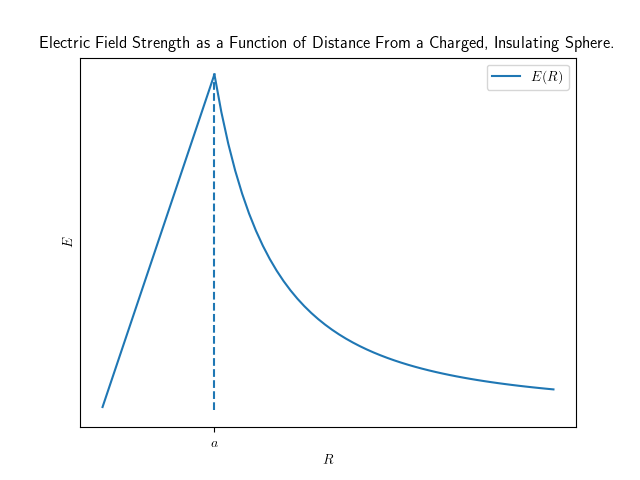
\includegraphics[scale=0.4]{electric_field_insulating_sphere.png}
            \caption{The electric field strength as a function of distance from the centre of a charged insulating sphere.}
            \label{fig:electric field strength insulating sphere}
        \end{subfigure}
        \begin{subfigure}{0.4\textwidth}
            \centering
            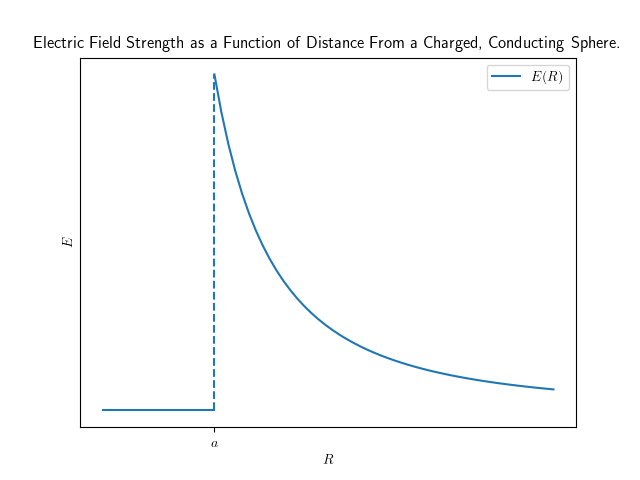
\includegraphics[scale=0.4]{electric_field_conducting_sphere.png}
            \caption{The electric field strength as a function of distance from the centre of a charged conducting sphere.}
            \label{fig:electric field strength conducting sphere}
        \end{subfigure}
        \caption{Electric field strength due to insulating and conducting spheres.}
    \end{figure}
    \subsubsection{Conducting Sphere}
    Consider now the same set up as above but the sphere is made of a conductor.
    Outside of the sphere all of the same logic applies and so for \(R > a\) we have
    \[E(R) = \frac{Q}{4\pi\varepsilon_0}\frac{1}{R^2} = \frac{\rho a^3}{3\varepsilon_0 R^2}.\]
    Inside the sphere the electric field is zero so we have \(E(R) = 0\) for \(R < a\).
    This is plotted in figure~\ref{fig:electric field strength conducting sphere}.
    
    \subsection{Cylindrical Symmetry}
    Take an infinitely long, thin wire with uniform charge density, \(\lambda\).
    We argue that by the symmetry of the situation the electric field must be
    \[\vv{E}(\vv{r}) = E(\rho)\ve{\rho}\]
    where we are working in cylindrical coordinates, \((\rho, \varphi, z)\).
    The argument for this is similar to the spherical case.
    If we place the origin on the wire, this is the only sensible choice for the location of the origin, then we are free to place it anywhere along the wire and we can define \(\varphi = 0\) as any position around the wire.
    This means that the field cannot depend on \(z\) or \(\varphi\) as then the origin position we pick would effect the field strength which is non-physical.
    Similarly if there is a component in the \(\ve{\varphi}\) direction then it must be the same all the way around the cylinder which means that there is a closed loop in the electric field meaning that \(\curl\vv{E} \ne \vv{0}\) which cannot be the case in an electrostatics situation.
    Finally the field can't have a component in the \(\ve{z}\) direction as this would cause motion of charge along the wire which would result in the charge distribution not being uniform.
    Therefore we are left only with dependence on \(\rho\) and a component in the direction \(\ve{\rho}\).
    
    Now construct a Gaussian surface of a cylinder of radius \(\rho\) which shares an axis with the wire.
    The field is always normal to this surface over the curved part so
    \[\vv{E}\cdot\dd{\vv{S}} = E(\rho)\ve{\rho}\cdot\dd{S}\ve{\rho} = E(\rho)\dd{S}.\]
    Over the flat ends of the cylinder the field is parallel to the surface so for the top surface
    \[\vv{E}\cdot\dd{\vv{S}} = E(\rho)\ve{\rho}\cdot\dd{S}\ve{z} = 0,\]
    the case of the bottom surface is the same but \(\dd{S}\) is negative.
    From Gauss' law we then have
    \begin{align*}
        \frac{Q_\mathrm{enc}}{\varepsilon_0} &= \oint_A \vv{E}\cdot\dd{\vv{S}}\\
        &= E(\rho)\int_{\mathrm{CSA}}\dd{S}\\
        &= E(\rho)2\pi\rho L
    \end{align*}
    where \(\mathrm{CSA}\) is the curved surface area of the cylinder and \(L\) is the length of the cylinder.
    The charge enclosed is simply \(Q_\mathrm{enc} = \lambda L\) so rearranging the above equation gives us
    \[E(\rho) = \frac{\lambda L}{\varepsilon}\frac{1}{2\pi\rho L} = \frac{\lambda}{2\pi\rho\varepsilon_0}.\]
    This is plotted in figure~\ref{fig:electric field strength of a charged wire}.
    \begin{figure}[ht]
        \centering
        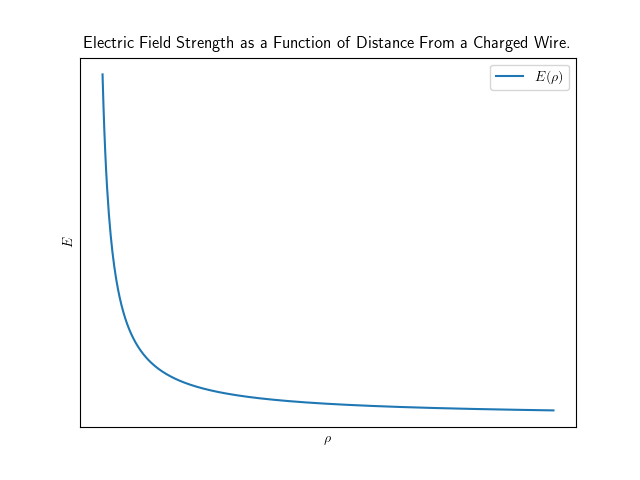
\includegraphics[scale=0.6]{electric_field_wire.png}
        \caption{The electric field strength due to a charged wire.}
        \label{fig:electric field strength of a charged wire}
    \end{figure}
    
    \subsection{Planar Symmetry}
    \subsubsection{Insulating Plane}
    Take an infinite plane with uniform charge density \(\sigma\).
    By symmetry we argue that
    \[\vv{E}(\vv{r}) = E(z)\ve{z}\]
    where we define \(\ve{z}\) as normal to the plane and place the origin in the plane.
    The argument for this is, again, similar to the previous arguments.
    Since we are free to place the origin anywhere in the plane there can be no \(x\) or \(y\) dependence in the field.
    We are also free to rotate the axis around the \(z\) axis which means that any component in the \(\ve{x}\) or \(\ve{y}\) direction must form a complete loop in the electric field which would mean \(\curl\ve{E} \ne \vv{0}\), this is not possible in electrostatics so there must be no \(\ve{x}\) or \(\ve{y}\) components.
    
    We choose a Gaussian surface that is a cylinder of radius \(R\).
    We place it so that its flat faces are parallel to the plane and one is above the plane and the other below.
    As well as this we have both faces the same distance from the plane.
    
    Along the curved surface the field is parallel to the surface so \(\vv{E}\cdot\dd{\vv{S}} = 0\).
    On the top face
    \[\vv{E}\cdot\dd{\vv{S}} = E(z)\ve{z}\cdot\dd{S}\ve{z} = E(z)\dd{S}.\]
    For the bottom case we have \(z < 0\).
    Since we are free to define \(z\)-axis in either direction we must have mirror symmetry in the \((x, y)\)-plane meaning that \(E(-z) = -E(z)\).
    This means that for the bottom face of the cylinder we have
    \[\vv{E}\cdot\dd{\vv{S}} = E(z)\ve{e}\cdot(-\dd{S}\ve{e}) = -E(z)\dd{S}.\]
    However since \(z < 0\) we have \(E(z) = E(-\abs{z}) = -E(\abs{z})\) so
    \[\vv{E}\cdot\dd{\vv{S}} = E(\abs{z})\dd{S}.\]
    This means that the contribution from the two faces is equal to twice the contribution from the top face.
    Applying Gauss' law we have
    \begin{align*}
        \frac{Q_\mathrm{enc}}{\varepsilon_0} &= \oint_A\vv{E}\cdot\dd{\vv{S}}\\
        &= E(z)\int_{2\circ}\dd{S}\\
        &= 2\pi R^2E(z)
    \end{align*}
    where \(2\circ\) is the two circular faces.
    The charge enclosed is \(Q_\mathrm{enc} = \pi R^2\sigma\) so rearranging the above equation gives us
    \[E(z) = \sgn(z)\frac{Q_\mathrm{enc}}{2\pi R^2\varepsilon_0} = \sgn(z)\frac{\pi R^2\sigma}{2\pi R^2\varepsilon_0} = \sgn(z)\frac{\sigma}{2\varepsilon_0},\]
    where
    \[
        \sgn(z) = 
        \begin{cases}
            1, & z > 0,\\
            0, & z = 0,\\
            -1, & z < 0.
        \end{cases}
    \]
    Notice that the only dependence on \(z\) is which side of the plane we are on as that affects the direction of the field.
    The field strength is constant.
    There is a discontinuous jump of \(\sigma/\varepsilon_0\) as we move from one side of the plane to the other.
    This is plotted in figure~\ref{fig:electric field insulated plane}
    \begin{figure}[ht]
        \centering
        \begin{subfigure}{0.4\textwidth}
            \centering
            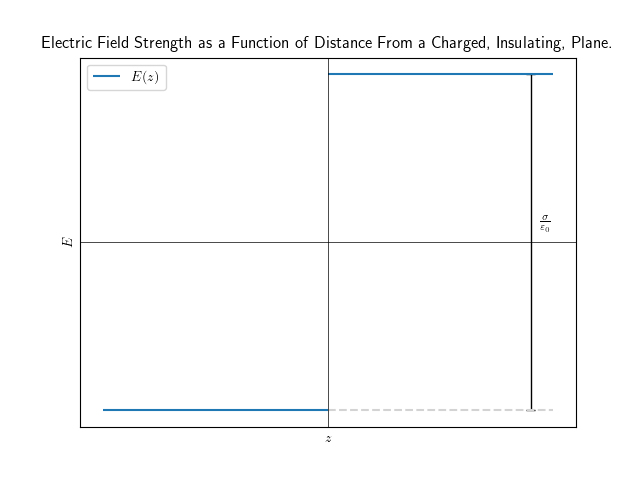
\includegraphics[scale=0.4]{electric_field_insulating_plane.png}
            \caption{Electric field strength as a function of distance from an insulating charged plane.}
            \label{fig:electric field insulated plane}
        \end{subfigure}
        \begin{subfigure}{0.4\textwidth}
            \centering
            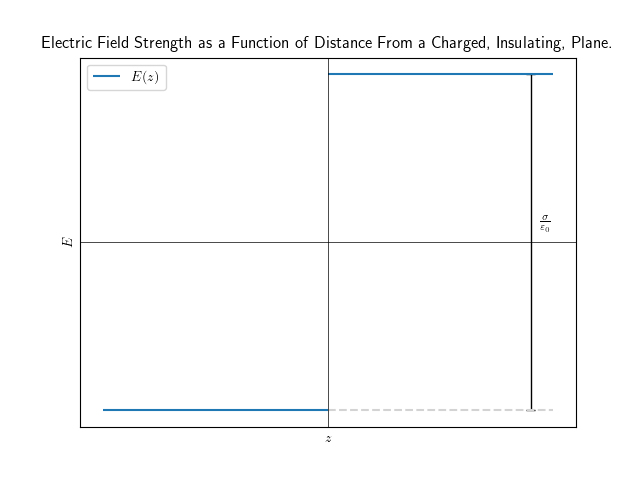
\includegraphics[scale=0.4]{electric_field_insulating_plane.png}
            \caption{Electric field strength as a function of distance from an insulating charged plane.}
            \label{fig:electric field conducting plane}
        \end{subfigure}
        \caption{Electric field strength due to insulating and conducting spheres.}
    \end{figure}
    If instead we have a conducting, charged, plane then the situation is a little different.
    By a conducting plane what we mean is that the plane is the surface of a conductor that continues on below the plane forever.
    The same logic as before works above the plane but now we have that the electric field below the plane is zero as it is inside a conductor.
    Thus
    \begin{align*}
        \frac{Q_\mathrm{enc}}{\varepsilon_0} &= \oint_A\vv{E}\cdot\dd{\vv{S}}\\
        &= E(z)\int_\circ \dd{S},\qquad z > 0\\
        &= E(z)\pi R^2\\
    \end{align*}
    So the electric field strength is
    \[
        E(z) = \begin{cases}
            \frac{\sigma}{\varepsilon_0}, & z > 0,\\
            0, & z \le 0.
        \end{cases}
    \]
    This is plotted in figure~\ref{fig:electric field conducting plane}.
    Note that in both cases there is a discontinuity of \(\sigma/\varepsilon_0\) when passing from one side of the plane to the other.
    
    \section{Poisson's Equation}
    \acrfull{pe} is a \acrfull{pde} of the form
    \[\laplacian\varphi = f\]
    where \(\varphi, f\colon\reals^3\to\reals\).
    The specific case of \(f(\vv{r}) = 0\) gives us
    \[\laplacian\varphi = 0\]
    which is \acrfull{le}.
    This crops up a lot in \acrshort{em} as the electrostatic potential and electric field are connected by
    \[\vv{E} = -\grad V\]
    and the electric field and charge density are related by Gauss' law:
    \[\div\vv{E} = \frac{\rho}{\varepsilon_0}.\]
    Combining these we get
    \[\div(\grad V) = \laplacian V = -\frac{\rho}{\varepsilon_0}.\]
    This simplifies to \acrshort{le} if \(\rho = 0\) everywhere in the region of interest.
    
    The most obvious solution to Laplace's equation is a potential of \(V(\vv{r}) = V_0\) for some constant \(V_0\).
    However as with all \acrshort{pde} there will be a set of \acrfull{bc} and typically \(V(\vv{r}) = V_0\) won't satisfy these \acrshort{bc}.
    Both \acrshort{pe} and \acrshort{le} are among the most important \acrshort{pde} in physics and appear in many scenarios.
    
    \subsection{Properties of Poisson's Equation}
    If \(V(\vv{r})\) is known then it is trivial to compute \(\rho(\vv{r}) = -\varepsilon\laplacian V\) or \(\vv{E}(\vv{r}) = -\grad V\).
    The more likely scenario however is that we know \(\rho(\vv{r})\) and we want to find the electric field.
    The first thing we should attempt should be to use Gauss' law, however this requires high levels of symmetry to be the most useful method.
    Lacking this symmetry the next thing that we can try to do is solve \acrshort{pe} for the potential.
    There is an explicit solution, given by the original definition of the potential:
    \[V(\vv{r}) = \frac{1}{4\pi\varepsilon_0}\int\frac{\rho(\vv{r'})}{\abs{\vv{r} - \vv{r'}}}\dd[3]{r'}.\]
    However this integral often has no analytic solution.
    There are methods for solving it numerically but this is not a numerical methods course so we won't discuss them.
    
    There are two useful properties of \acrshort{pe} that we use to find solutions:
    \begin{enumerate}
        \item The first useful property is linearity.
        If \(V_1\) and \(\rho_1\) satisfy \acrshort{pe} and \(V_2\) and \(\rho_2\) satisfy \acrshort{pe} then \(V_1 + V_2\) and \(\rho_1 + \rho_2\) satisfy \acrshort{pe}.
        That is
        \[\laplacian(V_1 + V_2) = -\frac{1}{\varepsilon_0}(\rho_1 + \rho_2).\]
        This follows trivially from the linearity of \(\laplacian\) as an operator which in turn follows from the linearity of partial derivatives as operators.
        In terms of \acrshort{em} this is just a restatement of the superposition principle.
        One use of this is if we have a shaped charge distribution, \(\rho\), that can be created from simpler shaped charged distributions, \(\rho_i\), then we can find the potential of each individual charge distribution and sum them together to get the potential of the entire charge distribution.
        For example a charged plane with a circular hole can be thought of as a plane without a hole and a charged disc the size of the hole, at the same position but with the opposite charge to the plane over he same area.
        
        \item The second useful property is that the solution to \acrshort{pe} is unique (possibly up to a constant term) for a given set of \acrshort{bc}.
        There are two common ways that \acrshort{bc} are given:
        \begin{itemize}
            \item \(V\) is specified on the boundary -- known as Dirichlet \acrshort{bc}.
            The solution will be unique.
            \item \(\vv{E}\) is specified on the boundary -- known as Neumann \acrshort{bc}.
            The solution will be unique up to a constant term.
        \end{itemize}
    \end{enumerate}
    
    \subsubsection{Proof of Uniqueness}
    \begin{theorem}
        Consider a region, \(\region\), with boundary, \(\boundary\)\footnote{It is possible that the boundary could be at infinity.}.
        Let \(\rho(\vv{r})\) be specified within \(\region\).
        Let the \acrshort{bc} be given by either
        \begin{enumerate}
            \item \(V\) is specified on \(\boundary\).
            \item \(\vv{E} = -\grad V\) is specified on \(\boundary\).
        \end{enumerate}
        Then any solution of \acrfull{pe},
        \[\laplacian V = -\frac{\rho}{\varepsilon_0},\]
        which satisfies the boundary conditions is unique (up to a constant term in the case of the second set of boundary conditions.)
    \end{theorem}
    \begin{proof}
        Suppose that \(V_1\) and \(V_2\) are two distinct solutions to \(\laplacian V = -\rho/\varepsilon_0\).
        Define \(\psi = V_1 - V_2\).
        Then
        \begin{align*}
            \laplacian \psi &= \laplacian(V_1 - V_2)\\
            &= \laplacian V_1 - \laplacian V_2\\
            &= \rho - \rho\\
            &= 0.
        \end{align*}
        Thus \(\psi\) is a solution to \acrshort{le}.
        Multiplying by \(\psi\) we have
        \[\psi\laplacian\psi = \psi\cdot0 = 0.\]
        Consider the following:
        \[\div(\psi\grad\psi) - (\grad\psi)\cdot(\grad\psi)\]
        Applying the product rule for the divergence of the product of a scalar field and vector field to the first term we get
        \[(\div\psi)\cdot(\div\psi) - \psi(\div(\grad\psi) - (\grad\psi)\cdot(\grad\psi).\]
        The first and last terms cancel and we are left with
        \[\psi(\div(\grad\psi)) = \psi\laplacian\psi = 0.\]
        So the whole term is zero over the whole of \(\region\).
        This means that integrating this term over \(\region\) will also be zero:
        \[\int_\region \div(\psi\grad\psi) - (\grad\psi)\cdot(\grad\psi)\dd{V} = 0.\]
        Applying the divergence theorem to the first term this becomes
        \[\int_\boundary \psi\grad\psi\cdot\dd{\vv{S}} - \int_\region (\grad\psi)\cdot(\grad\psi) \dd{V} = 0.\]
        For either set of boundary conditions the first term is zero.
        The second term is nonnegative everywhere as the integrand is the norm of a vector.
        Therefore for the integral to be zero we must have that the integrand is zero.
        The norm of a vector is only zero when that vector is zero therefore
        \[\grad\psi = 0.\]
        This means that \(\psi = V_1 - V_2\) is constant.
        So \(V_1\) and \(V_2\) differ by at most a constant.
        If the boundary conditions were given in terms of \(V\) at \(\boundary\) then we know that \(V_1 = V_2\) at the boundaries so this constant is zero.
    \end{proof}
    
    \begin{example}
        Consider a cavity, \(\region\), in a conductor.
        We claim that if \(\rho = 0\) in the cavity then \(\vv{E} = \vv{0}\) inside the cavity.
        
        The inner surface of the conductor is an equipotential since it is conducting.
        This means that \(V = V_0\) for some constant \(V_0\).
        This is our \acrshort{bc}.
        Inside the cavity we have \(\laplacian V = 0\) since there is no charge.
        Thus we have to solve \acrshort{le} subject to the condition that \(V = V_0\) on the boundary.
        One solution to this is \(V = V_0\) everywhere in \(\region\).
        By the uniqueness theorem above we know that this is the only solution.
        Now we simply compute \(\vv{E} = -\grad V = -\grad V_0 = \vv{0}\).
    \end{example}
    
    \subsection{The Method of Images}
    The method of images is a method for solving \acrshort{pe} by placing `image charges' outside of the region, \(\region\), such that they reproduce the required \acrshort{bc}.
    These charges don't affect \acrshort{pe} inside \(\region\) as they aren't in the region so don't change \(\rho\) in the region.
    However the field that results from the superposition of these image charges as well as any pre-existing charges is the correct solution to \acrshort{pe}.
    
    \begin{example}
        Consider a conducting plane with a point charge, \(Q\), placed a distance \(a\) above the plane.
        What is the potential in the region, \(\region\), above the plane?
        
        The charge density above the plane is
        \[\rho(\vv{r}) = Q\delta(z - a)\delta(x)\delta(y)\]
        where we have placed the origin in the plane directly below the charge and have the \(z\)-axis normal to the plane.
        Our boundary condition is that \(V(x, y, 0) = 0\) as at the plane \(\vv{E} = 0\) so \(V = V_0\) and we choose \(V_0 = 0\) for simplicity.
        
        Unfortunately \(V = V_0\) is not a solution to \acrshort{pe} here as we know that the potential from a point charge falls away as \(1/r\) so at the origin (in the plane directly below the charge) we expect the potential to be \(V = 1/a\) of what it is at the point charge.
        We need to solve
        \[\laplacian V(\vv{r}) = -\frac{\rho(\vv{r})}{\varepsilon_0}.\]
        To do this we can add a homogenous solution, \(V_\text{im}\) to \acrshort{pe}.
        By homogenous here we mean that \(\laplacian V_\text{im} = 0\), i.e. a solution to \acrshort{le}.
        This solution only needs to be homogeneous for \(z \ge 0\) since this is the region of interest.
        We know that the potential due to the point charge is
        \[V_Q(\vv{r}) = \frac{Q}{r\pi\varepsilon_0}\frac{1}{\sqrt{x^2 + y^2 + (z - a)^2}}.\]
        We place an image charge, \(-Q\), at \(z = -a\) which gives us an image potential of
        \[V_\text{im}(\vv{r}) = -\frac{Q}{r\i\varepsilon_0}\frac{1}{\sqrt{x^2 + y^2 + (z + a)^2}}.\]
        At every point on the plane we have
        \[V_Q + V_\text{im} = \frac{Q}{r\i\varepsilon_0}\frac{1}{\sqrt{x^2 + y^2 + (0 - a)^2}} - \frac{Q}{r\i\varepsilon_0}\frac{1}{\sqrt{x^2 + y^2 + (0 + a)^2}} = 0\]
        so the boundary conditions are satisfied.
        Thus \(V = V_Q + V_\text{im}\) is the solution and gives the potential everywhere.
        
        In reality this potential isn't caused by two point charges.
        Rather the real point charge causes the charge density of the plane to become non-uniform in a way that the final potential is as given above.
    \end{example}
    
    \section{Electric Dipoles and Multipoles}
    The motivation behind this section is to study a general, non-trivial, charge distribution, \(\rho(\vv{r})\), and in particular find an approximation of the potential,
    \[V(\vv{r}) = \frac{1}{4\pi\varepsilon_0}\int\frac{\rho(\vv{r'})}{\abs{\vv{r} - \vv{r'}}}\dd[3]{r'},\]
    which applies to points, \(\vv{r}\), far from where \(\rho(\vv{\vv{r'}}) \ne 0\).
    
    \subsection{Electric Dipoles}
    An \define{electric dipole} is formed from two charges, \(\pm q\), fixed distance \(a\) apart.
    The vector from \(q\) to \(-q\) is defined to be \(\vv{a}\).
    The \define{electric dipole moment} is then defined to be \(\vv{p} = q\vv{a}\).
    An electric dipole is shown in figure~\ref{fig:electric dipole}.
    \begin{figure}[ht]
        \centering
        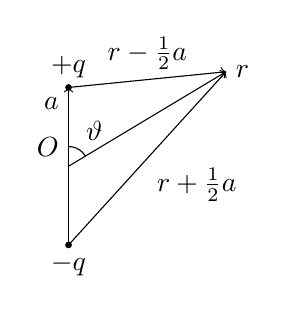
\begin{tikzpicture}
            \draw[fill=black] (0, 1) circle[radius=0.035cm];
            \draw[fill=black] (0, -1) circle[radius=0.035cm];
            \node[above] at (0, 1) {\(+q\)};
            \node[below] at (0, -1) {\(-q\)};
            \node[above left] at (0, 0) {\(O\)};
            \draw[->] (0, -1) -- (0, 1);
            \node[below left] at (0, 1) {\(\vv{a}\)};
            \draw[->] (0, 1) -- (2, 1.2);
            \draw[->] (0, -1) -- (2, 1.2);
            \draw[->] (0, 0) -- (2, 1.2);
            \node[right] at (2, 1.2) {\(\vv{r}\)};
            \begin{scope}
                \clip (0, 0) -- (0, 1) -- (2, 1.2) -- cycle;
                \draw (0, 0) circle[radius=0.25cm];
            \end{scope}
            \node[above right] at (0.1, 0.2) {\(\vartheta\)};
            \node[above] at (1, 1.1) {\(\vv{r} - \frac{1}{2}\vv{a}\)};
            \node[below right] at (1, 0.1) {\(\vv{r} + \frac{1}{2}\vv{a}\)};
        \end{tikzpicture}
        \caption{An electric dipole.}
        \label{fig:electric dipole}
    \end{figure}
    Dipoles like this are important because many molecules, such as \ce{H2O} and \ce{CO} have permanent dipoles and all molecules/atoms acquire an induced dipole in an external field.
    
    \subsubsection{Field of an Electric Dipole}
    The electric potential of an electric dipole is simply the superposition of the potential due to the two point charges:
    \[V(\vv{r}) = \frac{q}{4\pi\varepsilon_0}\left(\frac{1}{r_+} - \frac{1}{r_-}\right)\]
    where 
    \[\vv{r_{\pm}} = \vv{r} \mp \frac{1}{2}\vv{a}.\]
    That is \(\vv{r_\pm}\) is the vector from \(\pm q\) to \(\vv{r}\).
    The next question that we ask is what is the field like for \(r \gg a\)?
    This is known as the far field approximation.
    We can Taylor expand the \(1/r_\pm\) terms in the potential.
    To do this we first note that
    \begin{align*}
        r_\pm^2 &= \vv{r_\pm}\cdot\vv{r_\pm}\\
        &= \left(\vv{r} \mp \frac{1}{2}\vv{a}\right)\cdot\left(\vv{r} \mp \frac{1}{2}\vv{a}\right)\\
        &= r^2 \mp \vv{a}\cdot\vv{r} + \frac{1}{4}a^2\\
        &= r^2 \mp  ar\cos\vartheta + \frac{1}{4}a^2\\
        &= r^2\left(1 \mp \frac{a}{r}\cos\vartheta + \frac{a^2}{4r^2}\right).
    \end{align*}
    Hence
    \[\frac{1}{r_\pm} = \left[r^2\left(1 \mp \frac{a}{r}\cos\vartheta + \frac{a^2}{4r^2}\right)\right]^{-1/2} = \frac{1}{r}\left[\left(1 \mp \frac{a}{r}\cos\vartheta + \frac{a^2}{4r^2}\right)\right]^{-1/2}.\]
    For \(r > a\) this is of the form \((1 + \varepsilon)^p\) with \(\abs{\varepsilon} < 1\) needed to use
    \[(1 + \varepsilon)^p = 1 + p\varepsilon + \order{\varepsilon^2}.\]
    Doing this gives
    \begin{align*}
        \frac{1}{r_\pm} &= \frac{1}{r}\left[1 - \frac{1}{2}\left(\mp\frac{a}{r}\cos\vartheta + \frac{a^2}{4r^2}\right) + \order{\frac{a^2}{r^2}}\right]\\
        &= \frac{1}{r} \pm \frac{a}{2r^2}\cos\vartheta + \order{\frac{a^2}{r^3}}.
    \end{align*}
    Substituting this into the potential gives
    \begin{align*}
        V(\vv{r}) &= \frac{q}{4\pi\varepsilon_0}\left(\frac{1}{r_+} - \frac{1}{r_-}\right)\\
        &\approx \frac{q}{4\pi\varepsilon_0}\left(\frac{1}{r} + \frac{a}{2r^2}\cos\vartheta - \frac{1}{r} + \frac{a}{2r^2}\cos\vartheta\right)\\
        &= \frac{qa\cos\vartheta}{r^2\pi\varepsilon_0}\\
        &= \frac{\vv{p}\cdot\vh{r}}{4\pi\varepsilon_0r^2}.
    \end{align*}
    Notice that this drops off as \(1/r^2\) whereas the potential from a point charge drops off slower as \(1/r\).
    You can think of this as the fact that there are positive and negative charges close together causing parts of the potential to cancel.
    What we have derived here is the far field limit, in that it is only valid for \(r \gg a\).
    It is also known as the `ideal dipole' potential which is what we would get if we too a limit as \(a \to 0\), and \(q\to\infty\) in such a way that \(\vv{p}\) remains constant.
    
    \subsubsection{Dipole Interaction With an External Electric Field}
    The electrostatic energy of a point charge, \(q\), in a potential, \(V\), is \(U = qV\).
    The energy of a dipole is then the superposition of the two point charges:
    \[U_\text{dip} = qV_\text{ext}(\vv{a}/2) - qV_\text{ext}(-\vv{a}/2).\]
    Here \(V_\text{ext}\) is the external potential.
    Taking a Taylor series gives
    \begin{align*}
        U_\text{dip} &\approx q\left[V_\text{ext}(0) + \frac{1}{2}\vv{a}\cdot\grad V_\text{ext}\right] - q\left[V_\text{ext}(0) - \frac{1}{2}\vv{a}\cdot\grad V_\text{ext}\right]\\
        &= q\vv{a}\cdot\grad V_\text{ext}\\
        &= -q\vv{a}\cdot\vv{E_\mathrm{ext}}\\
        &= -p\cdot\vv{E_\mathrm{ext}}
    \end{align*}
    We see that the dipole energy is minimised if \(\vv{p}\) is parallel to \(\vv{E_\mathrm{ext}}\) and the energy is maximised when they are antiparallel.
    The change in energy to change between parallel and antiparallel is
    \[\Delta U = 2p\abs{E_\mathrm{ext}}.\]
    The force experienced by the dipole is
    \[\vv{F} = -\grad U_\text{dip} = \grad(\vv{p\cdot\vv{E_\mathrm{ext}}}).\]
    If \(\vv{E_\mathrm{ext}}\) is a uniform field (doesn't depend on \(\vv{r}\)) then the force is zero.
    This is because the two charges experience equal and opposite forces.
    However there is still a torque because the two charges aren't in the same location.
    This torque acts to align the dipole with \(\vv{E_\mathrm{ext}}\) and is given by:
    \[\vv{\tau} = \frac{1}{2}\vv{a}\times q\vv{E_\mathrm{ext}} - \frac{1}{2}\vv{a}\times(-q\vv{E_\mathrm{ext}}) = \vv{p}\times\vv{E_\mathrm{ext}}.\]
    The work done by the torque to rotate the dipole from aligned with the field to an angle \(\vartheta\) from the field is
    \[W = \int_0^\vartheta \tau\dd{\vartheta} = \int_0^\vartheta qE_\mathrm{ext}\dd{\vartheta} = pE_\mathrm{ext}(1 - \cos\vartheta).\]
    In a non-uniform field the force is generally more complex.
    It acts to move the dipole along the gradient of the field.
    
    \subsection{Multipole Expansion}
    Given a charge distribution \(\rho\) we say that \(\rho\) is bounded inside a region, \(\region\), if, for \(\vv{r}\notin\region\), \(\rho(\vv{r}) = 0\).
    Let \(\rho\) be a charge distribution that is bounded inside the region \(\region\).
    Then from the definition of the potential we know that
    \[V(\vv{r}) = \frac{1}{4\pi\varepsilon_0} \int_\region \frac{\rho(\vv{r'})}{\abs{\vv{r} - \vv{r'}}}\dd[3]{r'}.\]
    This holds for all \(\vv{r}\).
    However if \(\vv{r}\notin\region\), that is \(r \gg r'\), then we can make use of a Taylor expansion.
    Following the same steps as we did for a dipole we see that
    \[\frac{1}{\abs{\vv{r} - \vv{r'}}} = \frac{1}{r}\left[1 - \frac{2\vv{r}\cdot\vv{r'}}{r^2} + \frac{r'^2}{r^2}\right]^{-1/2}.\]
    We now Taylor expand this but keep higher order terms:
    \begin{align*}
        \left[1 - \frac{2\vv{r}\cdot\vv{r'}}{r^2} + \frac{r'^2}{r^2}\right]^{-1/2} &= 1 - \frac{1}{2}\left(-\frac{2\vv{r}\cdot\vv{r'}}{r^2} + \frac{r'^2}{r^2}\right) + \frac{3}{8}\left(-\frac{2\vv{r}\cdot\vv{r'}}{r^2} + \frac{r'^2}{r^2}\right)^2 + \order{\frac{1}{r^3}}\\
        &= 1 + \frac{\vv{r}\cdot\vv{r'}}{r^2} - \frac{1}{2}\frac{r'^2}{r^2} + \frac{3}{2}\frac{(\vv{r}\cdot\vv{r'})^2}{r^4} - \frac{3}{2}\frac{r'^2(\vv{r}\cdot\vv{r'})}{r^4} - \frac{3}{8}\frac{r'^4}{r^4} + \order{\frac{1}{r^3}}\\
        &= 1 + \frac{\vh{r}\cdot\vv{r'}}{r} - \frac{1}{2}\frac{r'^2}{r^2} + \frac{3}{2}\frac{(\vh{r}\cdot\vv{r'})^2}{r^2} - \frac{3}{2}\frac{r'^2(\vh{r}\cdot\vv{r})}{r^3} - \frac{3}{8}\frac{r'^4}{r^4} + \order{\frac{1}{r^3}}
        \shortintertext{keeping only terms of order \(1/r^2\) or lower}
        &\approx 1 + \frac{\vh{r}\cdot\vv{r'}}{r} - \frac{1}{2}\frac{r'^2}{r^2} + \frac{3}{4}\frac{(\vh{r}\cdot\vv{r'})^2}{r^2}\\
        &= 1 + \frac{\vh{r}\cdot\vv{r'}}{r} + \frac{3(\vh{r}\cdot\vv{r'}) - r'^2}{2r^2}
    \end{align*}
    Using this in the definition of the potential gives
    \begin{align*}
        V(\vv{r}) &\approx \frac{1}{4\pi\varepsilon_0}\int_\region \dd[3]{r'} \rho(\vv{r'})\frac{1}{r}\left[1 + \frac{\vh{r}\cdot\vv{r'}}{r} + \frac{3(\vh{r}\cdot\vv{r'}) - r'^2}{2r^2}\right]\\
        &= \frac{1}{4\pi\varepsilon_0}\int_\region \dd[3]{r'} \rho(\vv{r'})\left[\frac{1}{r} + \frac{\vh{r}\cdot\vv{r'}}{r^2} + \frac{3(\vh{r}\cdot\vv{r'}) - r'^2}{2r^3}\right].
    \end{align*}
    Defining some new terms this becomes
    \[V(\vv{r}) \approx \frac{1}{4\pi\varepsilon_0}\frac{Q}{r} + \frac{1}{r\pi\varepsilon_0}\frac{\vh{r}\cdot\vv{P}}{r^2} + \frac{1}{4\pi\varepsilon_0}\frac{1}{r^3}\frac{1}{2}\sum_{i, j}\quadrupole_{ij}\hat{r}_i\hat{r}_j.\]
    Where
    \[Q = \int_\region \dd[3]{r'}\rho(\vv{r'})\]
    is the total charge,
    \[\vv{P} = \int_\region \dd[3]{r'}\vv{r'}\rho(\vv{r'})\]
    is the net dipole moment, a vector with Cartesian components
    \[P_i = \int_\region \dd[3]{r'}r'_i\rho(\vv{r'}),\]
    and \(\quadrupole\) is the quadrupole tensor which has Cartesian components
    \[\quadrupole_{ij} = \int_\region\dd[3]{r'}(3r'_ir'_j - r'^2\delta_{ij})\rho(\vv{r'}).\]
    This representation of \(V\) is the \define{multipole expansion} of \(V\) in Cartesian coordinates.
    The first term is the monopole term.
    It is dominant when \(Q\ne 0\) and reasonably approximates the far field charge distribution as a point charge at the origin.
    When the total charge, \(Q\), is zero then the second term, the dipole term, dominates.
    If this term also vanishes then the third term, the quadrupole term, dominates.
    Note that another way of writing this terms is
    \[\frac{1}{4\pi\varepsilon_0}\frac{1}{r^3}\frac{1}{2} \vh{r}\trans\quadrupole\vh{r} = \frac{1}{4\pi\varepsilon_0}\frac{1}{r^5}\frac{1}{2} \vv{r}\trans\quadrupole\vv{r}.\]
    It is possible to take even more terms of the Taylor series and end up with more terms, however we will stop at three.
    Note that each term of the expansion is a solution to \gls{le} and therefore we can use the method of images with image dipoles and quadrupoles as well as image charges.
    
    \begin{example}\label{exa:dipole moment}
        \begin{figure}[ht]
            \centering
            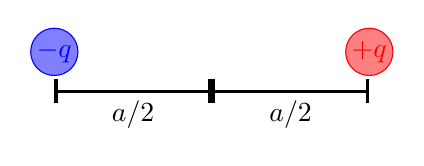
\begin{tikzpicture}
                \draw[color=red, fill=red!50!white] (2, 0) circle[radius=0.3cm];
                \draw[color=blue, fill=blue!50!white] (-2, 0) circle[radius=0.3cm];
                \draw[very thick, |-|] (-2, -0.5) -- (0, -0.5);
                \draw[very thick, |-|] (0, -0.5) -- (2, -0.5);
                \node[red] at (2, 0) {\(+q\)};
                \node[blue] at (-2, 0) {\(-q\)};
                \node[below] at (-1, -0.5) {\(a/2\)};
                \node[below] at (1, -0.5) {\(a/2\)};
            \end{tikzpicture}
            \caption{The dipole setup used in example~\ref{exa:dipole moment}}
        \end{figure}
        A dipole formed of two charges, \(\pm q\), aligned along the \(x\)-axis so that \(q\) is at \((a/2, 0, 0)\) and \(-q\) is at \((-a/2, 0, 0)\) has a charge density given by
        \[\rho(\vv{r}) = q[\delta(x - a/2) - \delta(x + a/2)]\delta(y)\delta(z).\]
        Clearly \(Q = 0\).
        The \(x\) component of the dipole moment is
        \begin{align*}
            P_x &= \int x\rho(\vv{r})\dd{V}\\
            &= q\int x[\delta(x - a/2) - \delta(x + a/2)]\dd{x}\int\delta(y)\dd{y}\int\delta(z)\dd{z}\\
            &= q\frac{a}{2} - q\left(\frac{a}{2}\right)\\
            &= qa.
        \end{align*}
        The \(y\) component is
        \begin{align*}
            P_y &= \int y\rho(\vv{r})\dd{V}\\
            &= \int[\delta(x - a/2) - \delta(x + a/2)]\dd{x}\int y\delta(y)\dd{y}\int \delta(z)\dd{z}\\
            &= 0
        \end{align*}
        since the middle integral is zero.
        Similarly we can show that \(P_z = 0\).
        This means that \(\vv{P} = q\vv{a}\), so we are justified in calling \(\vv{P}\) the dipole moment.
    \end{example}
    \begin{example}\label{exa:quadrupole moment}
        \begin{figure}[ht]
            \centering
            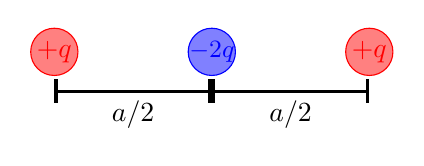
\begin{tikzpicture}
                \draw[color=red, fill=red!50!white] (-2, 0) circle[radius=0.3cm];
                \draw[color=red, fill=red!50!white] (2, 0) circle[radius=0.3cm];
                \draw[color=blue, fill=blue!50!white] (0, 0) circle[radius=0.3cm];
                \node[color=red] at (-2, 0) {\(+q\)};
                \node[color=red] at (2, 0) {\(+q\)};
                \node[color=blue] at (0, 0) {\small\(-2q\)};
                \draw[very thick, |-|] (-2, -0.5) -- (0, -0.5);
                \draw[very thick, |-|] (0, -0.5) -- (2, -0.5);
                \node[below] at (-1, -0.5) {\(a/2\)};
                \node[below] at (1, -0.5) {\(a/2\)};
            \end{tikzpicture}
            \caption{The quadrupole setup used in example~\ref{exa:quadrupole moment}}
        \end{figure}
        Three charges are placed in a line along the \(x\)-axis.
        Two of the charges have charge \(q\) and are at \(\pm a/2\).
        The third charge is at the origin and has charge \(-2q\).
        The charge density is
        \[\rho(\vv{r}) = q[\delta(x - a/2) + \delta(x + a/2) - 2\delta(x)]\delta(y)\delta(z).\]
        Again, \(Q = 0\).
        The \(x\) component of the dipole moment is
        \begin{align*}
            P_x &= \int x\rho(\vv{r})\dd{V}\\
            &= q\int x[\delta(x - a/2) + \delta(x + a/2) - 2\delta(x)]\int\delta(y)\dd{y}\int\delta(z)\dd{z}\\
            &= q\left[\frac{a}{2} - \frac{a}{2} + 0\right]\\
            &= 0
        \end{align*}
        In a similar way to the previous example \(P_y = P_z = 0\).
        Thus the dipole moment vanishes.
        
        Next we calculate the quadrupole moment.
        In general
        \[\quadrupole_{ij} = \int(3x_ix_j - r^2\delta_{ij})\rho(\vv{r})\dd{V}.\]
        The \(\quadrupole_{xx}\) component is
        \begin{align*}
            \quadrupole_{xx} &= \int(3x^2 - r^2)q[\delta(x - a/2) + \delta(x + a/2) - 2\delta(x)]\delta(y) \delta(z)\dd{V}\\
            &= \int(3x^2 - (x^2 + y^2 + z^2))q[\delta(x - a/2) + \delta(x + a/2) - 2\delta(x)]\delta(y) \delta(z)\dd{V}\\
            &= 3q\left(\frac{a}{2}\right)^2 - q\left(\frac{a}{2}\right)^2 + 3q\left(-\frac{a}{2}\right)^2 - q\left(-\frac{a}{2}\right)^2\\
            &= qa^2
        \end{align*}
        Next we will calculate \(\quadrupole_{xy}\):
        \begin{align*}
            \quadrupole_{xy} &= \int 3xyq[\delta(x - a/2) + \delta(x + a/2) - 2\delta(x)]\delta(y) \delta(z)\dd{V}\\
            &= \int 3xq[\delta(x - a/2) + \delta(x + a/2) - 2\delta(x)]\dd{x}\int y\delta(y)\dd{y} \int\delta(z)\dd{z}\\
            &= 0
        \end{align*}
        If we calculated every component we would find that
        \[
            \quadrupole = qa^2
            \begin{pmatrix}
                1 & 0 & 0\\
                0 & -\frac{1}{2} & 0\\
                0 & 0 & -\frac{1}{2}
            \end{pmatrix}
            .
        \]
        We can then approximate the potential as
        \begin{align*}
            V(\vv{r}) &= \frac{1}{8\pi\varepsilon_0} \frac{1}{r^5}\vv{r}\trans\quadrupole\vv{r}\\
            &= \frac{qa^2}{8\pi\varepsilon_0}\frac{1}{r^5}
            \begin{pmatrix}
                x & y & z
            \end{pmatrix}
            \begin{pmatrix}
                1 & 0 & 0\\
                0 & -\frac{1}{2} & 0\\
                0 & 0 & -\frac{1}{2}
            \end{pmatrix}
            \begin{pmatrix}
                x\\ y\\ z
            \end{pmatrix}
            \\
            &= \frac{qa^2}{8\pi\varepsilon_0}\frac{1}{r^5}
            \begin{pmatrix}
                x & y & z
            \end{pmatrix}
            \begin{pmatrix}
                x\\ -\frac{1}{2}y\\ -\frac{1}{2}z
            \end{pmatrix}
            \\
            &= \frac{qa^2}{8\pi\varepsilon_0}\frac{1}{r^5}
            \left[x^2 - \frac{1}{2}(y^2 + z^2)\right].
        \end{align*}
    \end{example}
    \begin{example}\label{exa:quadrupole moment 2}
        \begin{figure}[ht]
            \centering
            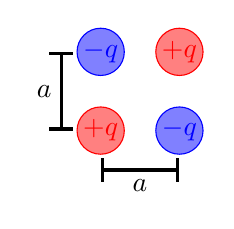
\begin{tikzpicture}
                \draw[color=red, fill=red!50!white] (0, 0) circle[radius=0.3cm];
                \draw[color=blue, fill=blue!50!white] (1, 0) circle[radius=0.3cm];
                \draw[color=blue, fill=blue!50!white] (0, 1) circle[radius=0.3cm];
                \draw[color=red, fill=red!50!white] (1, 1) circle[radius=0.3cm];
                \node[color=red] at (0, 0) {\(+q\)};
                \node[color=blue] at (1, 0) {\(-q\)};
                \node[color=blue] at (0, 1) {\(-q\)};
                \node[color=red] at (1, 1) {\(+q\)};
                \draw[very thick, |-|] (0, -0.5) -- (1, -0.5);
                \draw[very thick, |-|] (-0.5, 0) -- (-0.5, 1);
                \node[below] at (0.5, -0.5) {\(a\)};
                \node[left] at (-0.5, 0.5) {\(a\)};
            \end{tikzpicture}
            \caption{The quadrupole setup used in example~\ref{exa:quadrupole moment 2}}
        \end{figure}
        Four charges \(\pm q\) are placed on the corners of a square in the \((x, y)\)-plane with side length \(a\) with the origin at the centre of the square.
        They are arranged such that diagonally opposite charges have the same sign and charges connected by an edge have opposite signs.
        The charge density is
        
        \begin{multline*}
            \rho(\vv{r}) = q[\delta(x - a/2)\delta(y - a/2) - \delta(x + a/2)\delta(y - a/2) \\- \delta(x - a/2)\delta(y + a/2) + \delta(x + a/2)\delta(y + a/2)]\delta(z).
        \end{multline*}
        Again it can be shown that \(\vv{P} = \vv{0}\) and clearly \(Q = 0\).
        If we calculate the quadrupole components then we find that
        \[
            \quadrupole = qa^2
            \begin{pmatrix}
                0 & 3 & 0\\
                3 & 0 & 0\\
                0 & 0 & -2
            \end{pmatrix}
            .
        \]
        The potential can then be approximated as
        \[V(\vv{r}) = \frac{qa^2}{8\pi\varepsilon_0}\frac{1}{r^5}[6xy - 2z^2].\]
    \end{example}

    \section{Electrostatic Energy and Capacitors}
    \subsection{Electrostatic Energy of a General Charge Distribution}\label{sec:energy electric field}
    If we start with an assembly of \(n - 1\) point charges, \(q_i\), at position \(\vv{r_i}\) then the potential at \(\vv{r}\) is given by the superposition of the potentials of each particle:
    \[V(\vv{r}) = \frac{1}{4\pi\varepsilon_0}\sum_{j=1}^{n-1}\frac{q_i}{\abs{\vv{r} - \vv{r_j}}}.\]
    If we then bring another charge, \(q_n\), from infinity to \(\vv{r_n}\) then the work required to do so is
    \[W_n = q_nV(\vv{r_n}) = \frac{q_n}{\frac{q_n}{4\pi\varepsilon_0}} \sum_{j=1}^{n-1}\frac{q_j}{\abs{\vv{r_n} - \vv{r_j}}}.\]
    We can write out this sum for the first few values of \(n\) to see how it progresses:
    \begin{align*}
        W_1 &= 0\\
        W_2 &= \frac{q_2q_1}{4\pi\varepsilon_0}\frac{1}{\abs{\vv{r_2} - \vv{r_1}}}\\
        W_3 &= \frac{q_3q_1}{4\pi\varepsilon_0}\frac{1}{\abs{\vv{r_3} - \vv{r_1}}} + \frac{q_3q_2}{4\pi\varepsilon_0}\frac{1}{\abs{\vv{r_3} - \vv{r_2}}}
    \end{align*}
    In general the total work required to assemble \(n\) charges, which is the electrostatic energy, \(U_E\), is given by
    \begin{align*}
        U_E &= \sum_{i=1}^{n}W_i\\
        &= \frac{1}{4\pi\varepsilon_0}\sum_{i=1}^{n}\sum_{j=1}^{i - 1}\frac{q_iq_j}{\abs{\vv{r_i} - \vv{r_j}}}\\
        &= \frac{1}{8\pi\varepsilon_0}\sum_{\stackrel{i, j}{i\ne j}}^{n}\frac{q_iq_j}{\abs{\vv{r_i} - \vv{r_j}}}.
    \end{align*}
    In the last step we collapsed two sums into one by noting that a sum over \(i\) and \(j\) with \(i > j\) is equivalent to a sum over \(i\) and \(j\) with \(i \ne j\) except that the second allows for \((i,j) = (2,1)\) and \((i,j)=(1,2)\).
    Due to symmetry the value of both of these terms is the same so we end up double counting the allowed states where \(i > j\) if we include all \(j \ne i\).
    For this reason we have to divide by 2 which explains the factor of \(8\) in the denominator.
    
    In the limit of a continuous charge density, \(\rho\), the electrostatic energy is
    \[U_E = \frac{1}{2}\int\rho(\vv{r})V(\vv{r})\dd[3]{r}.\]
    Using Maxwell's first law this becomes
    \[U_E = \frac{\varepsilon_0}{2}\int V(\vv{r})(\div\vv{E})\dd[3]{r}.\]
    We then use the product rule,
    \[\div(V\vv{E}) = V\div\vv{E} + (\grad V)\cdot\vv{E} = V\div\vv{E} - \vv{E}\cdot\vv{E} = V\div\vv{E} - E^2,\]
    to change the integrand to
    \[U_E = \frac{\varepsilon_0}{2}\int \div[V(\vv{r})\vv{E}(\vv{r})] + E^2\dd[3]{r}.\]
    Splitting the integral at the addition and applying the divergence theorem to the first integral we get
    \[U_E = \frac{\varepsilon_0}{2}\oint_SV(\vv{r})\vv{E}(\vv{r})\cdot\dd{\vv{S}} + \frac{\varepsilon_0}{2}\int E^2\dd[3]{r}.\]
    So far we have made no assumptions about the volume over which our integration occurs.
    This means we are free to pick any boundary, \(S\).
    We choose \(S\) to be at infinity.
    Assuming that our charge distribution is bound we know that outside of the region containing it \(V\) drops of as at least \(1/r\) and \(E\) drops off as at least \(1/r^2\).
    Thus \(VE\) drops of as at least \(1/r^3\).
    The area of the surface however only grows as \(1/r^2\) so the first integral must be zero.
    Thus the internal energy is
    \[U_E = \frac{\varepsilon_0}{2}\int \abs{\vv{E}(\vv{r})}^2\dd[3]{r} = \int u_E \dd[3]{r},\]
    where
    \[u_E = \frac{\varepsilon_0}{2}\abs{\vv{E}(\vv{r})}^2\]
    is the energy density.
    
    Note that this derivation started from a continuous charge distribution.
    This does not apply to point charges.
    If we were to apply it to point charges there are self interaction terms that we would have to exclude.
    We can see this form the point charge equations, if we try to include the interaction of a point charge with itself we get \(\abs{\vv{r_i} - \vv{r_i}} = 0\) so we end up dividing by zero.
    We are now assuming that the integral is over all space, if we wish to only consider a small volume we either require that \(E = 0\) outside of that area or we have to consider the first integral that we reasoned to be zero for an infinite volume.
    As a final warning the electrostatic energy is quadratic in field strength so the superposition principle \emph{does not} apply to energy densities.
    
    \subsection{Capacitors}
    A capacitor comprises of two neighbouring conducting bodies with equal and opposite charges, \(\pm Q\).
    The capacitance is defined to be
    \[C = \frac{Q}{V}\]
    where \(V\) is the potential difference between the two bodies.
    This is well defined as the surfaces of the conductors are equipotentials so it doesn't matter where we select on each conductor to measure the potential difference.
    
    \subsubsection{Parallel Plate Capacitors}
    The simplest capacitor is a parallel plate capacitor where we model the two conductors as thin, infinite, parallel, planes a distance \(d\) apart.
    We can easily calculate the field from the superposition of the fields from two charged planes.
    The set up and electric field from each plate is shown in figure~\ref{fig:parallel plate capacitor electric field}.
    The magnitude of the field from each plate is the same and equal to \(\sigma/2\varepsilon_0\), it is also the same everywhere.
    This is important because it means that between the plates where the fields align the net field is \(\sigma/\varepsilon_0\).
    However outside of the plates the fields are anti-aligned and cancel so the net field is 0.
    \begin{figure}[ht]
        \centering
        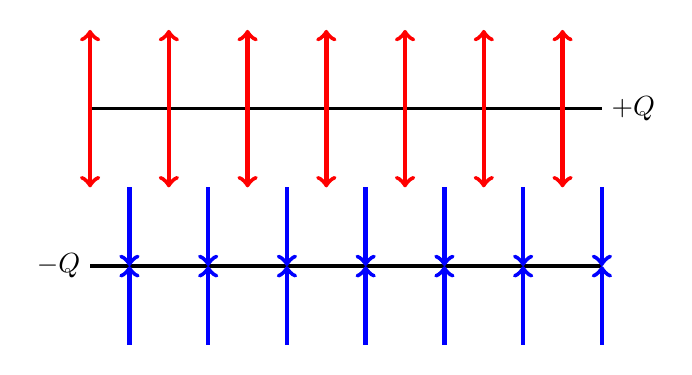
\begin{tikzpicture}
            \draw[very thick] (0, 0) -- (6.5, 0);
            \draw[very thick] (0, 2) -- (6.5, 2);
            \foreach \x in {0,...,6} {
                \begin{scope}[color=red, ultra thick]
                    \draw[->] (\x, 2) -- (\x, 1);
                    \draw[->] (\x, 2) -- (\x, 3);
                \end{scope}
                \begin{scope}[xshift=0.5cm, color=blue, ultra thick]
                    \draw[->] (\x, 1) -- (\x, 0);
                    \draw[->] (\x, -1) -- (\x, 0);
                \end{scope}
            }
            \node[right] at (6.5, 2) {\(+Q\)};
            \node[left] at (0, 0) {\(-Q\)};
        \end{tikzpicture}
        \caption{Parallel plate capacitor electric field.}
        \label{fig:parallel plate capacitor electric field}
    \end{figure}
    The potential difference between the fields is given by
    \[V = -\int_0^d E_z\dd{z} = \frac{\sigma}{\varepsilon_0}d = \frac{Qd}{A\varepsilon_0}\]
    where we have chosen a coordinate system such that \(\ve{z}\) is normal to the plates and points from the negative to the positive plate.
    The origin is also chosen to be in the negative plate.
    The area of each plate is \(A\).
    The capacitance is then given by
    \[C = \frac{Q}{V} = \frac{A\varepsilon_0}{d}.\]
    Notice that the capacitance depends only on the geometry of the plates (their area and the distance between) it is independent of the charge and potential difference.
    It turns out that in general capacitance is a purely geometric property.
    
    We can use the charge distribution to calculate the electrostatic energy of the charged capacitor.
    \begin{align*}
        U_E &= \frac{1}{2}Q(V_1 - V_2)\\
        &= \frac{1}{2}QV\\
        &= \frac{1}{2}\frac{Q^2}{E}
    \end{align*}
    We can also use the fact that the electric field vanishes outside of the plates to calculate the electrostatic energy of the charged capacitor.
    \begin{align*}
        U_E &= \frac{\varepsilon_0}{2}\int E^2\dd[3]{r}\\
        &= \frac{\varepsilon_0}{2} \left(\frac{\sigma}{\varepsilon_0}\right)^2 \int\dd[3]{r}\\
        &= \frac{\sigma^2}{2\varepsilon_0}dA\\
        &= \frac{dQ^2}{2\varepsilon_0A}\\
        &= \frac{1}{2}\frac{Q^2}{E}.
    \end{align*}
    Here we have used that the empty integral is just the volume which in this case since \(E = 0\) outside of the capacitor is just the volume between the plates, \(dA\).
    
    \subsubsection{Edge Effects}
    \textit{This section is non-examinable}
    
    So far we have assume that the plates are infinite and therefore the fields are uniform between the plates.
    However in reality the plates cannot be infinite.
    For a finite sized capacitor the field bulges out of the capacitor and isn't uniform between the plates.
    
    Suppose that instead of infinite planes the capacitor is made from two discs of radius \(R\).
    We can perform an integral over the charge distribution to obtain the potential a height \(z\) above the disc:
    \[V(z) = \frac{1}{4\pi\varepsilon_0}\int_S\frac{\sigma}{(\rho^2 + z^2)^{1/2}}\dd{S}.\]
    In plane polar coordinates \(\dd{S} = \rho\dd{\rho}\dd{\varphi}\) so
    \begin{align*}
        V(z) &= {\sigma}{4\pi\varepsilon_0} \int_{0}^{2\pi} \dd{\varphi} \int_0^R \dd{\rho} \frac{\rho}{(\rho^2 + z^2)^{1/2}}\\
        &= \frac{\sigma}{4\pi\varepsilon_0}2\pi\left[(\rho + z^2)^{1/2}\right]_{\rho=0}^{\rho=R}\\
        &= \frac{\sigma}{2\varepsilon_0}\left[(R^2 + z^2)^{1/2} - z\right].
    \end{align*}
    This means that the \(z\) component of the electric field is
    \[E_z = -\pdv{V}{z} = -\frac{\sigma}{2\varepsilon_0}\left[\frac{z}{(R^2 + z^2)^{1/2}} - 1\right].\]
    This depends on \(z\) so the field is not uniform between the plates.
    There are two interesting limiting cases.
    First \(R \ll z\):
    \begin{align*}
        \vv{E}(R) &= \frac{\sigma}{2\varepsilon_0}\left[1 - \left(1 + \frac{R^2}{z^2}\right)^{-1/2}\right]\ve{z}
        \shortintertext{Taylor expanding the binomial term gives}
        &\approx \frac{\sigma}{2\varepsilon_0}\left[1 - \left(1 - \frac{1}{2}\frac{R^2}{z^2}\right)\right]\ve{z}\\
        &= \frac{\sigma R^2}{4\varepsilon_0 z^2}\ve{z}\\
        &= \frac{Q}{4\pi\varepsilon_0 z^2}\ve{z}
    \end{align*}
    where \(Q = \sigma\pi R^2\) is the total charge.
    We see that in this limit we can essentially view the capacitors as a point charge when we are far enough away that we can approximate it as having no volume.
    
    The other interesting case is when \(R \gg z\).
    In this case the term \(z / (R^2 + z^2)^{-1/2}\approx 0\) so
    \[\vv{E}(R) = \frac{\sigma}{2\varepsilon_0}\ve{z}.\]
    So in the case that the discs are very large they approximate infinite planes.
    It is only when \(R\approx z\) (i.e. \(A\approx d^2\)) that we need to consider the edge effects of the capacitor.
    Fortunately in practice this is rarely necessary.
        \part{Magnetostatics}
    \section{The Magnetic Field}
    \subsection{The Magnetic Force}
    The \define{magnetic field}, \(\vv{B}\), is defined by the force, \(\vv{F}\), experienced by a charge, \(q\), with velocity \(\vv{v}\), in an external electric field \(\vv{E}\):
    \[\vv{F} = q(\vv{E} + \vv{v}\times\vv{B}).\]
    This is called the \define{Lorentz force law}.
    The units of \(\vv{B}\) are teslas, \si{\tesla}, defined by \(\SI{1}{\tesla} = \SI{1}{\newton.\ampere^{-1}.\metre^{-1}}\).
    This is quite a large unit and it is common to use an alternative unit called a gauss defined by \(\SI{e-4}{\tesla} = \SI{1}{\gauss}\) sometimes also denoted \(\SI{1}{\gaussAlternate}\).
    
    The important thing about this formula is that the force due to the magnetic field, \(\vv{v}\times\vv{B}\), is perpendicular to the velocity.
    This means that magnetic fields do no work as \(\vv{v}\cdot(\vv{v}\times\vv{B}) = \vv{0}\).
    
    \subsection{Current}
    A \define{current} is a moving density of charge.
    For a \define{steady current} at any point, \(\vv{r}\), a constant (time independent) density of charge moves past \(\vv{r}\) in a given time.
    Steady currents are important as if all currents are steady we will see that this leads to a constant magnetic field in the same way that stationary charges lead to a constant electric field.
    A current formed by \(n(\vv{r})\) charges, \(q\), moving past the point \(\vv{r}\) with average velocity \(\vv{v}(\vv{r})\) can be described by a \define{current density}
    \[\vv{J}(\vv{r}) = n(\vv{r})q\vv{v}(\vv{r}) = \rho(\vv{r})\vv{v}(\vv{r}).\]
    Here we have used \(n(\vv{r})q = \rho(\vv{r})\).
    The current density is to the magnetic field as the charge density is to the electric field.
    The units of \(\vv{J}\) are \(\si{\ampere.\metre^{-2}}\).
    We can similarly define a surface current density, usually denoted \(\vv{K}\) or \(\vv{j}\).
    This will have units of \(\si{\ampere.\metre^{-1}}\).
    We can also define a line current density, usually denoted \(\vv{I}\), which has units of \(\si{\ampere}\).
    
    The total current, \(I\), is the current density through a surface, \(A\):
    \[I = \int_A \vv{J}\cdot\dd{\vv{S}},\]
    where \(\dd{\vv{S}}\) is a surface element normal to \(A\).
    
    \begin{example}
        An insulating disc of radius \(R\) with uniform charge density, \(\sigma\), is rotated about its axis with an angular velocity, \(\vv{\omega} = \omega\ve{z}\).
        As a result the disc has a surface current density:
        \[\vv{K} = \sigma\vv{v} = \sigma\vv{\omega}\vv{r} = \sigma\omega\ve{z}\times r\ve{\rho} = \sigma\omega r\ve{\varphi}.\]
        Notice that this is a steady current even though the disc is moving faster towards the edge, hence scaling with \(r\).
        The important thing for a steady current is that the current is constant at any one point in space, not that it has the same value at all points of space.
    \end{example}
    
    \subsection{Conductivity}
    The \define{conductivity}, \(\sigma\), is an intrinsic bulk property of a material.
    It relates the current density to the electric field:
    \[\vv{J} = \sigma\vv{E}.\]
    This is \define{Ohm's law}.
    This assumes that \(\vv{J}\) and \(\vv{E}\) are parallel.
    This is only the case if the material is isotropic, that is all directions within the material are equivalent.
    If this isn't the case then we need to use the conductivity tensor, \(\sigma_{ij}\), instead.
    
    A typical value of \(\sigma\) for a metal is \(\SI{e9}{\ohm^{-1}.\metre^{-1}}\).
    We define the \define{resistivity} as
    \[\rho = \frac{1}{\sigma}.\]
    A typical value of \(\rho\) for an insulator is \(\SI{e16}{\ohm.\metre}\).
    In a superconductor \(\rho = 0\).
    
    Suppose a wire of cross sectional area \(A\) has a homogenous current density and electric field.
    The current in the wire is
    \[I = \int_A\vv{J}\cdot\dd{\vv{S}} = \int_A J\dd{S} = \int \sigma E\dd{S} = E\sigma A.\]
    The potential difference between two points on the wire a distance \(d\) apart is
    \[\Delta V = Ed.\]
    The current can then be written as
    \[I = \frac{A\sigma}{d}\Delta V.\]
    Rearranging we get
    \[\Delta V = IR,\qquad\text{where}\qquad R = \frac{d\rho}{A}.\]
    \(R\) here is what we define as the \define{resistance}.
    It has units of ohms, \(\si{\ohm}\).
    This equation is the more familiar form of Ohm's law.
    
    \subsection{Current Elements}
    A current element, \(\dd{\vv{\current}}\), is a vector defined by
    \begin{align*}
        \dd{\vv{\current}(\vv{r})} &= \vv{J}(\vv{r})\dd{V},\\
        \dd{\vv{\current}(\vv{r})} &= \vv{K}(\vv{r})\dd{S},\\
        \dd{\vv{\current}(\vv{r})} &= \vv{I}(\vv{r})\dd{l}.
    \end{align*}
    The units of a current element are \(\si{\ampere.\metre}\).
    Be careful, \(\vv{K}\dd{S} \ne K\dd{S}\), the first points in the direction of the surface current density, which is along the surface, and the second is normal to the surface.
    On the other hand \(\vv{I}\dd{l} = I\dd{\vv{l}}\) since a line current element always points along the line and so does a line element.

    A current is a moving charge element.
    For a bulk current density we have
    \[\dd{\vv{\current}}(\vv{r}) = \vv{J}(\vv{r})\dd{V} = \rho(\vv{r})\vv{v}(\vv{r})\dd{V} = \vv{v}(\vv{r})\dd{q}.\]
    This means that we can work out the force, \(\dd{\vv{F}}\), on a current element, \(\dd{\vv{\current}}\), in a magnetic field, \(\vv{B}\):
    \[\dd{\vv{F}} = \dd{q}\vv{v}\times\vv{B} = \dd{\vv{\current}}\times\vv{B}.\]
    If the current comes from a bulk current density, \(\dd{\vv{\current}} = \vv{J}\dd{V}\) then
    \[\dd{\vv{F}} = \vv{J}\times\vv{B}\dd{V}.\]
    
    \subsection{Biot Savart Law}
    The Biot Savart law is an empirical law relating current elements to the magnetic field.
    It states that if a current element \(\dd{\vv{\current}}(\vv{r'})\) is at position \(\vv{r'}\) then the resulting magnetic field at \(\vv{r}\) is given by
    \[\dd{\vv{B}(\vv{r})} = \frac{\mu_0}{4\pi} \frac{\dd{\vv{\current}(\vv{r'})} \times (\vv{r - \vv{r'}})}{\abs{\vv{r} - \vv{r'}}^3}.\]
    The Biot Savart law is to magnetic fields as Coulomb's law is to electric fields.
    It states that charge elements create magnetic fields which shows that a steady current causes a constant magnetic field.
    Here \(\mu_0\) is a constant known as the permeability of free space, or the electric constant.
    It has a value of
    \[\mu_0 = 4\pi\cdot\SI{e-7}{\henry.\metre^{-1}} = 4\pi\cdot\SI{e-7}{\newton.\ampere^{-2}}.\]
    Here \(\si{\henry}\) is a henry defined as \(\SI{1}{\henry} = \SI{1}{\newton.\metre.\ampere^{-2}}\).
    
    Since the Biot Savart law is linear in \(\dd{\vv{\current}}\) the superposition of the magnetic fields of many current elements to get the total magnetic fields holds so
    \[\vv{B}(\vv{r}) = \frac{\mu_0}{4\pi}\int \frac{\dd{\vv{\current}(\vv{r'})} \times (\vv{r} - \vv{r'})}{\abs{\vv{r} - \vv{r'}}^3}.\]
    For a bulk current density this becomes
    \[\vv{B}(\vv{r}) = \frac{\mu_0}{4\pi} \int \frac{\vv{J}(\vv{r'})\times(\vv{r} - \vv{r'})}{\abs{\vv{r} - \vv{r'}}^3} \dd[3]{r'}.\]
    
    \subsection{Magnetic Force Between Currents}
    The force on the current element \(\dd{\vv{\current_1}}\) at position \(\vv{r_1}\) due to a current element, \(\dd{\vv{\current_2}}\), at \(\vv{r_2}\) is
    \[\dd{\vv{F_1}} = \dd{\vv{\current_1}}\times\dd{\vv{B_2}} = \frac{\mu_0}{4\pi r_{12}^2} \dd{\vv{\current_1}} \times (\dd{\vv{\current_2}}\times \vhsub{r}{_{12}}).\]
    Here \(\dd{\vv{B_2}}\) is the magnetic field due to the second current element and \(\vv{r_{12}} = \vv{r_1} - \vv{r_2}\).
    If the each current element, \(\dd{\vv{\current_i}}\) is due to a bulk current density \(\vv{J_i}\) then this becomes
    \[\dd{\vv{F_1}} = \frac{\mu_0}{4\pi r_{12}^2} \vv{J_1}\times (\vv{J_2} \times \vhsub{r}{_{12}}) \dd[3]{r_1}\dd[3]{r_2}.\]
    
    \begin{example}
        A long straight wire is aligned along the \(z\)-axis.
        It carries a current, \(I\), in the positive \(z\) direction.
        What is the magnetic field strength at a point a distance \(r\) from the wire?
        
        A current element is given by
        \[\dd{\vv{\current}} = I\dd{z}\ve{z} = I\dd{\vv{r'}}\]
        where \(\vv{r'}\) is the position of the current element along the wire.
        Choosing the origin to be in the same plane as the point at which we are evaluating the field we have
        \[\vv{r} = \rho\ve{\rho}\]
        for the position at which we want to know the field strength (note that \(\rho\) here is cylindrical coordinates, not charge density or resistivity).
        Applying the Biot Savart law we get
        \begin{align*}
            \vv{B}(\vv{r}) &= \frac{\mu_0}{4\pi} \int \frac{\dd{\vv{\current}} \times (\vv{r} - \vv{r'})}{\abs{\vv{r} - \vv{r'}}^3}\\
            &= \frac{\mu_0}{4\pi} \int \frac{I\ve{z}\times(\rho\ve{\rho} - r'\ve{z})}{\abs{\vv{r} - \vv{r'}}^3} \dd{z}\\
            &= \frac{\mu_0}{4\pi} I \left[ \int \frac{\ve{z}\times\rho\ve{\rho}}{\abs{\vv{r} - \vv{r'}}^3} \dd{z} - \int \frac{\ve{z}\times r'\ve{z}}{\abs{\vv{r} - \vv{r'}}^3} \dd{z} \right]\\
            &= \frac{\mu_0 I}{4\pi}\rho\ve{\varphi}\int (\rho^2 + z^2)^{-3/2} \dd{z}\\
            &= \frac{\mu_0 I}{2\pi\rho}\ve{\varphi}.
        \end{align*}
        We looked up the integral in the last step over all \(z\in\reals\) and found it to be \(2/\rho^2\).
    \end{example}

    \section{Divergence and Curl of the Magnetic Field}
    \subsection{Divergence of the Magnetic Field}
    The Biot Savart law for a bulk current density, \(\vv{J}(\vv{r'})\), is
    \begin{align*}
        \vv{B}(\vv{r}) &= \frac{\mu_0}{4\pi} \int \vv{J}(\vv{r'}) \times \frac{(\vv{r} - \vv{r'})}{\abs{\vv{r} - \vv{r'}}^3} \dd[3]{r'}\\
        &= -\frac{\mu_0}{4\pi} \int \vv{J}(\vv{r'}) \times \grad_{\vv{r}}\left(\frac{1}{\abs{\vv{r} - \vv{r'}}}\right) \dd[3]{r'}
    \end{align*}
    Here we use a notation where differential operators with a subscript \(\vv{r}\) act only on the components of \(\vv{r}\).
    We can take the divergence of this fairly easily if we recognise that \(\vv{J}(\vv{r'})\) is constant with respect to \(\vv{r}\) so \(\grad_{\vv{r}}\cdot\vv{J}(\vv{r'}) = 0\).
    \begin{align*}
        \grad_{\vv{r}}\cdot\vv{B}(\vv{r}) &= -\frac{\mu_0}{4\pi} \int \grad_{\vv{r}}\cdot \left[\vv{J}(\vv{r'}) \times \grad_{\vv{r}}\left(\frac{1}{\abs{\vv{r} - \vv{r'}}}\right)\right] \dd[3]{r'}\\
        &= -\frac{\mu_0}{4\pi} \int \vv{J}(\vv{r'}) \cdot\left[\grad_{\vv{r}} \times \grad_{\vv{r}}\left(\frac{1}{\abs{\vv{r} - \vv{r'}}}\right)\right] \dd[3]{r'}\\
        &= 0
    \end{align*}
    Here we have used the identity that grad curl is zero.
    Hence
    \[\div\vv{B} = 0.\]
    This is \define{Maxwell's second law}.
    It states that there are no sinks or sources of the magnetic field,
    there are no magnetic monopoles, there are no point sources of the magnetic field, there are no `magnetic charges'.
    The magnetic field always forms closed loops.
    
    Applying the divergence theorem we have
    \[\int_V \div\vv{B}(\vv{r})\dd[3]{r} = \oint_A\vv{B}\cdot\dd{\vv{S}}.\]
    Identifying the left hand side as an integral of zero we have
    \[\oint_a\vv{B}\cdot\dd{\vv{S}} = 0.\]
    This is \define{Gauss' law for magnetic fields}.
    
    \subsection{Magnetic Dipoles}
    Maxwell's second law rules out the existence of magnetic monopoles.
    Therefore a magnetic dipole is the most elementary magnetic pole.
    It turns out that a magnetic dipole can be formed from a current loop.
    
    Suppose we have a circular loop or radius \(a\) carrying current \(I\).
    If we align the axis of the loop with the \(z\) axis so that the current is going in the \(\ve{\varphi}\) direction then the magnetic field on the axis can be found from the Biot Savart law,
    \[\dd{\vv{B}(\vv{r})} = \frac{\mu_0}{4\pi} \frac{\dd{\vv{\current}(\vv{r'})} (\vv{r} - \vv{r'})}{\abs{\vv{r} - \vv{r'}}^3}.\]
    Here \(\vv{r} = z\ve{z}\), \(\vv{r'} = a\ve{\rho}\), and \(\dd{\vv{\current}} = I\dd{\ell}\ve{\varphi}\).
    Hence
    \begin{align*}
        \dd{\vv{\current}} \times (\vv{r} - \vv{r'}) &= I\dd{\ell}\ve{\varphi} \times (z\ve{z} - a\ve{\rho})\\
        &= I\dd{\ell}(z\ve{\varphi}\times\ve{z} - a\ve{\varphi}\times\ve{\rho})\\
        &= I\dd{\ell}(z\ve{\rho} + a\ve{z}).
    \end{align*}
    Radial from diametrically opposed sides of the loop will cancel leaving a net field only in the \(\ve{z}\) direction:
    \[\dd{B_z} = \frac{\mu_0}{4\pi}\frac{Ia\dd{\ell}}{(a^2 + z^2)^{3/2}}\]
    Integrating this we get
    \begin{align*}
        B_z &= \frac{\mu_0}{4\pi} \frac{Ia}{(a^2 + z^2)^{3/2}} \oint\dd{\ell}\\
        &= \frac{\mu_0}{4\pi} \frac{Ia}{(a^2 + z^2)^{3/2}}2\pi a\\
        &= \frac{\mu_0Ia^2}{2(a^2 + z^2)^{3/2}}.
    \end{align*}
    At \(z = 0\) (i.e. the centre of the loop)
    \[B_z = \frac{\mu_0Ia^2}{2a^3} = \frac{\mu_0I}{2a}.\]
    In the far field (i.e. \(z \gg a\))
    \[B_z \approx \frac{\mu_0Ia^2}{2z^3}.\]
    It can be shown that off-axis field is
    \[\vv{B_{\mathrm{dip}}}(\vv{r}) = \frac{\mu_0}{4\pi r^3} [3(\vv{m}\cdot\vh{r})\vh{r} - \vv{m}]\]
    in the far field.
    Here \(\vv{m}\) is the dipole moment defined as
    \[\vv{m} = IA\ve{z}\]
    where \(A\) is the area of a current loop, in the \((x, y)\)-plane, and \(I\) is the current it carries.
    In this case \(A = \pi a^2\) so
    \[\vv{m} = I\pi a^2\ve{z}.\]
    More generally we can define the dipole moment as
    \[\vv{m} = I\vv{A} = I\int_A\dd{\vv{S}}\]
    where \(\vv{A}\) is the vector area of the loop defined by an integral over the entire loop, which may not be planar, and has surface elements \(\dd{\vv{S}}\).
    
    In an external magnetic field, \(\vv{B_\mathrm{ext}}\), a magnetic dipole has energy
    \[U = -\vv{m}\cdot\vv{B_\mathrm{ext}}.\]
    There is also a torque
    \[\vv{\tau} = \vv{m}\times\vv{B_\mathrm{ext}}.\]
    
    \subsection{Curl of the Magnetic Field}
    Starting again from the Biot Savart law for a bulk current density and this time taking the curl we have
    \[\grad_{\vv{r}} \times \vv{B}(\vv{r}) = -\frac{\mu_0}{4\pi} \int \grad_{\vv{r}} \times \left[\vv{J}(\vv{r'}) \times \grad_{\vv{r}}\left(\frac{1}{\abs{\vv{r} - \vv{r'}}}\right)\right] \dd[3]{r'}\]
    Looking just at the integrand we have
    \begin{align*}
        \grad_{\vv{r}} \times \left[\vv{J}(\vv{r'}) \times \grad_{\vv{r}}\left(\frac{1}{\abs{\vv{r} - \vv{r'}}}\right)\right] & = \vv{J}(\vv{r'})\laplacian_{\vv{r}}\left(\frac{1}{\abs{\vv{r} - \vv{r'}}}\right) - (\vv{J}(\vv{r'})\cdot\grad_{\vv{r}})\grad_{\vv{r}} \left(\frac{1}{\abs{\vv{r} - \vv{r'}}}\right)\\
        &= -4\pi\delta(\vv{r} - \vv{r'})\vv{J}(\vv{r'}) - (\vv{J}(\vv{r'})\cdot\grad_{\vv{r}}) \grad_{\vv{r}} \left(\frac{1}{\abs{\vv{r} - \vv{r'}}}\right).
    \end{align*}
    Hence the curl of the magnetic field is
    \begin{align*}
        \grad_{\vv{r}}\times\vv{B}(\vv{r}) &= \frac{\mu_0}{4\pi} \int 4\pi\delta(\vv{r} - \vv{r'})\vv{J}(\vv{r'}) \dd[3]{r'} + \frac{\mu_0}{4\pi} \int (\vv{J}(\vv{r'})\cdot\grad_{\vv{r}}) \grad_{\vv{r}} \left(\frac{1}{\abs{\vv{r} - \vv{r'}}}\right) \dd[3]{r'}
        \shortintertext{The second term can be shown to be zero by writing it as a boundary integral at infinity which must vanish to have finite energy}
        &= \frac{\mu_0}{4\pi} \int 4\pi\delta(\vv{r} - \vv{r'})\vv{J}(\vv{r'}) \dd[3]{r'}\\
        &= \mu_0\int \vv{J}(\vv{r'})\delta(\vv{r} - \vv{r'})\dd[3]{r'}\\
        &= \mu_0\vv{J}(\vv{r}).
    \end{align*}
    This is \define{Maxwell's fourth law}.
    Applying Stokes' theorem we have
    \[\int_S \curl\vv{B}\cdot\dd{\vv{S}} = \oint_C\vv{B}\cdot\dd{\vv{l}}.\]
    Looking at the left hand side we have
    \[\int_S \curl\vv{B}\cdot\dd{\vv{S}} = \mu_0 \int_S \curl\vv{J}\cdot\dd{\vv{S}} = \mu_0 I.\]
    Hence
    \[\oint_C\vv{B}\cdot\dd{\vv{l}} = \mu_0 I.\]
    This is \define{Ampere's law}.
    
    \begin{example}\label{exa:infinite wire magnetic field}
        Consider an infinite wire of radius \(a\) aligned along the \(\ve{z}\) direction carrying current density \(\vv{J}\propto\ve{z}\).
        We must have that \(B_z = 0\) as \(\vv{J}\) and \(\vv{B}\) must be perpendicular.
        Similarly we must have that \(B_\rho = 0\) as if there where radial components then \(\div\vv{B}\) would be non-zero violating the second of Maxwell's equations.
        Therefore \(\vv{B}\propto\ve{\varphi}\).
        Also \(B_\varphi\) cannot depend on \(z\) as we are free to place the origin anywhere along the wire and it cannot depend on \(\varphi\) as we are free to define any angle around the wire as \(\varphi = 0\).
        Thus we are left with
        \[\vv{B} = B_\varphi(\rho)\ve{\varphi}.\]
        For \(\rho > a\) we have
        \[\oint_C \vv{B}\cdot\dd{l} = B_\varphi 2\pi\rho = \mu_0 I_{\mathrm{enc}} = \mu_0 J\pi a^2.\]
        Hence
        \[B_\varphi = \frac{\mu_0 J}{2} \frac{a^2}{\rho}.\]
        For \(\rho < a\) we still have
        \[\oint_C \vv{B}\cdot\dd{\vv{l}} = B_\varphi 2\pi\rho\]
        but now
        \[\mu_0I_{\mathrm{enc}} = \mu_0J\pi\rho^2\]
        so
        \[B_\varphi = \frac{\mu_0J}{2}\rho.\]
        This is shown in figure~\ref{fig:magnetic field strength wire}.
        \begin{figure}[ht]
            \centering
            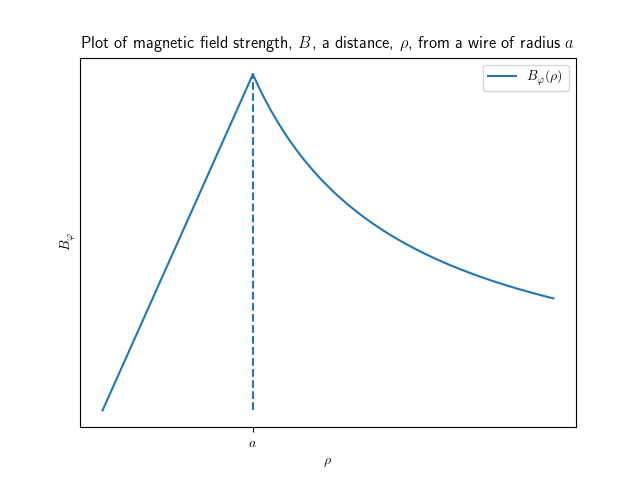
\includegraphics[scale=0.5]{magnetic_field_wire.png}
            \caption{The magnetic field strength a distance \(\rho\) from a wire.}
            \label{fig:magnetic field strength wire}
        \end{figure}
    \end{example}

    \section{Amp\`ere's Law and Vector Potentials}
    \subsection{Applications of Amp\`ere's Law}
    Amp\`ere's Law states
    \[\oint_C \vv{B}\cdot\dd{\vv{l}} = \mu_0 \int_A\vv{J}\cdot\dd{S} = \mu_0 I_\enc.\]
    Here \(\vv{B}\) is the magnetic field due to a current density \(\vv{J}\).
    \(C\) is some closed curve, called an Amp\`erian loop, bounding a surface \(A\) which has surface normals \(\dd{\vv{S}}\).
    \(I_\enc\) is the current that passes through the surface.
    The integration is performed along the curve in such a way that the surface normals and direction of integration agree with the right hand grip rule.
    Symmetry permitting Amp\`ere's law is usually the fastest way to calculate the magnetic field for a given current density.
    We look for cases where the Amp\`erian loop is either parallel or perpendicular to the magnetic field.
    The cases where this is possible and the Amp\`erian loops to use are
    \begin{itemize}
        \item Infinite straight line -- coaxial circles (see example~\ref{exa:infinite wire magnetic field})
        \item Infinite plane -- rectangular loop
        \item Infinite solenoid -- rectangular loop
        \item Toroid -- circle
    \end{itemize}
    \subsubsection{Infinite Slab of Current}
    An infinite slab of thickness \(d\) has a current density, \(\vv{J}\).
    Define the \(x\) direction to be the direction of this current density and the \(y\) direction to be in the slab but perpendicular to the current density and the \(z\) direction to be normal to the slab.
    
    The magnetic field cannot have an \(x\) component as the current density must be perpendicular to the magnetic field.
    The magnetic field cannot have a \(z\) component as if it did we could place a Gaussian surface with a section of the slab in it and the integral over it would be non-zero meaning that we would have non-vanishing divergence.
    This is forbidden by Maxwell's second law.
    This leaves us with a magnetic field that can only be in the \(y\) direction.
    
    If we choose to put the origin a distance \(d/2\) into the slab then since we can pick any point at this depth in the slab to place the origin we must have that \(B_y\) is independent of \(x\) and \(y\) and so \(B_y = B_y(z)\).
    
    We choose an Amp\`erian loop that is rectangular with two sides in the \(z\) direction and two in the \(y\) direction.
    The field is perpendicular to the sides in the \(z\) direction.
    The field is aligned with the sides in the \(y\) direction.
    Say that the length of these sides is \(b\), then
    \[\oint_C \vv{B}\cdot\dd{\vv{l}} = 2b\abs{B_y} = \mu_0I_\enc = \mu_0 bdJ\]
    \[\implies \abs{B_y} = \frac{1}{2}\mu_0 Jd.\]
    We know that \(\dd{\vv{\current}}\propto\ve{x}\) so for \(\vv{r}\propto\ve{z}\) we have, by the Biot Savart law, that
    \[\vv{B} \propto \vv{J}\times\vv{r} \propto \ve{x}\times\ve{z} = -\ve{y}\]
    This means that, outside of the slab, the magnetic field is
    \[
        \vv{B} =
        \begin{cases}
            -\frac{1}{2}\mu_0 Jd\ve{y}, & z > \frac{1}{2}d,\\
            +\frac{1}{2}\mu_0 Jd\ve{y}, & z < -\frac{1}{2}d.
        \end{cases}
    \]
    \begin{figure}[ht]
        \centering
        \tikzsetnextfilename{current-slab}
        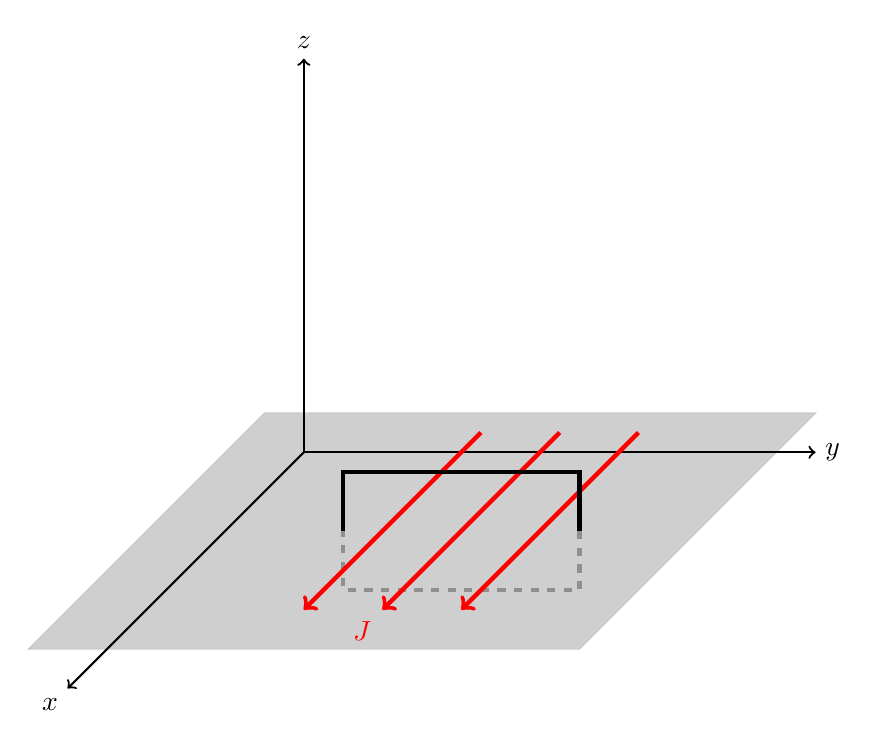
\begin{tikzpicture}
            \tikzstyle{current} = [color=red, ultra thick]
            \tikzstyle{axis} = [thick]
            \tikzstyle{conductor} = [color=lightgray, fill=lightgray, opacity=0.75]
            \tikzstyle{loop} = [ultra thick]
            \draw[dashed, loop] (3, -0.5) -- (3, -1.25) -- (0, -1.25) -- (0, -0.5);
            \draw[conductor] (-4, -2) -- (3, -2) -- (6, 1) -- (-1, 1) -- cycle;
            \begin{scope}[xshift=-0.5cm, yshift=0.5cm]
                \draw[axis, ->] (0, 0) -- (6.5, 0);
                \node[right] at (6.5, 0) {\(y\)};
                \draw[axis, ->] (0, 0) -- (0, 5);
                \node[above] at (0, 5) {\(z\)};
                \draw[axis, ->] (0, 0) -- (-3, -3);
                \node[below left] at (-3, -3) {\(x\)};
            \end{scope}
            \foreach \x in {0, 1, 2} {
                \draw[current, ->] (1.75 + \x, 0.75) -- (-0.5 + \x, -1.5);
            }
            \node[below left, current] at (0.5, -1.5) {\(\vv{J}\)};
            \draw[loop] (3, -0.5) -- (3, 0.25) -- (0, 0.25) -- (0, -0.5);
        \end{tikzpicture}
        \caption{Infinite slab of current}
    \end{figure}
    \begin{figure}[ht]
        \centering
        \tikzsetnextfilename{current-slab-2}
        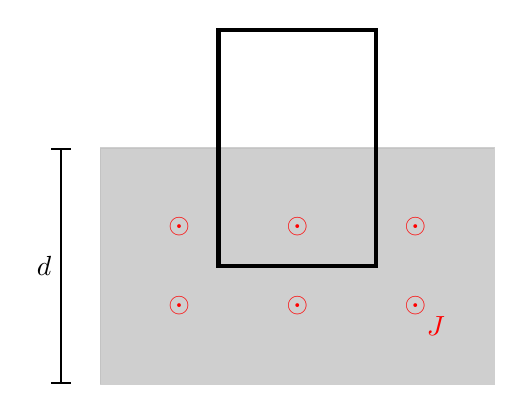
\begin{tikzpicture}
            \tikzstyle{current} = [color=red, ultra thick]
            \tikzstyle{conductor} = [color=lightgray, fill=lightgray, opacity=0.75]
            \tikzstyle{loop} = [ultra thick]
            \draw[conductor] (0, 0) rectangle (5, 3);
            %\draw (0, 0) grid (5, 3);
            \foreach \x in {1, 2.5, 4} {
                \foreach \y in {1, 2} {
                    \node[current] at (\x, \y) {\(\bm{\odot}\)};
                }   
            }
            \node[below right, current] at (4, 1) {\(\vv{J}\)};
            \draw[loop] (1.5, 1.5) rectangle (3.5, 4.5);
            \draw[thick, |-|] (-0.5, 0) -- (-0.5, 3);
            \node[left] at (-0.5, 1.5) {\(d\)};
        \end{tikzpicture}
        \caption{Finding the magnetic field inside a slab of current}
    \end{figure}
    If we want to know the magnetic field inside the slab then the set up for the Amp\'erian loop is similar but now one of the sides in the \(y\) direction should be inside the slab.
    We then use the field outside the loop that we already know to integrate along this loop.
    We find that
    \[B_{y,\text{in}} = -\mu_0Jz.\]
    \begin{figure}[ht]
        \centering
        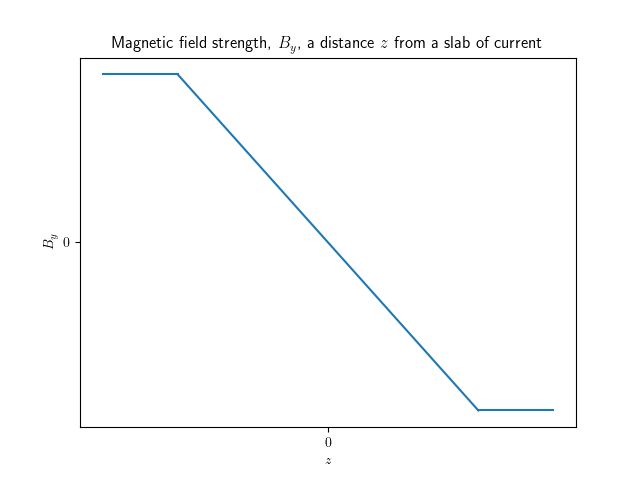
\includegraphics[scale=0.6]{magnetic_field_slab.png}
        \caption{The magnetic field strength, \(B_y\), a distance, \(z\), from a slab carrying current density, \(\vv{J}\).}
    \end{figure}

    \subsection{Toroid}
    A wire is curled up into a solenoid with \(n\) coils per unit length and radius \(R\).
    The solenoid is the curled up into a toroid of radius \(a > R\).
    \begin{figure}
        \centering
        \tikzsetnextfilename{toroid}
        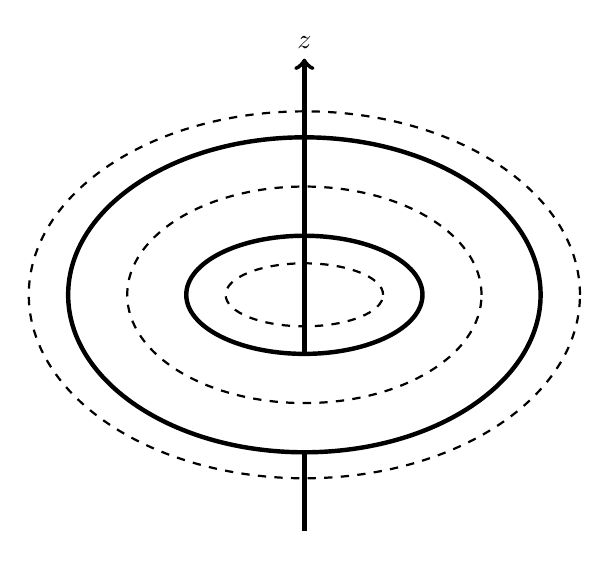
\begin{tikzpicture}
            \tikzstyle{axis} = [ultra thick]
            \tikzstyle{loop} = [thick, dashed]
            \tikzstyle{toroid} = [ultra thick]
            \draw[toroid] (0, 0) circle[x radius=3cm, y radius=2cm];
            \draw[toroid] (0, 0) circle[x radius=1.5cm, y radius=0.75cm];
            \draw[axis, ->] (0, -0.75) -- (0, 3);
            \draw[axis] (0, -2) -- (0, -3);
            \node[above] at (0, 3) {\(z\)};
            \draw[loop] (0, 0) circle[x radius=2.25cm, y radius=1.375cm];
            \draw[loop] (0, 0) circle[x radius=3.5cm, y radius=2.33cm];
            \draw[loop] (0, 0) circle[x radius=1cm, y radius=0.4cm];
        \end{tikzpicture}
        \caption{Finding the magnetic field inside a toroid}
        \label{fig:toroid}
    \end{figure}
    Figure~\ref{fig:toroid} shows a toroid (normal lines) with three possible Amp\'erian loops (dashed lines).
    The easiest loop to consider is the one that is entirely inside the hole of the toroid.
    Clearly there is no current enclosed in this so the magnetic field in the hole must be zero.
    Next we consider the outer most loop.
    At first it may seem like current does pass trough this but we must remember that the direction is important and therefore the \emph{net} current is zero as there is just as much current in both directions since the current is forming loops in the coil.
    Therefore outside of the toroid the magnetic field must be zero.
    The only Amp\'erian loop with a net current enclosed is the one that is in the toroid.
    
    All of the current element that pass through it are in the \((\rho, z)\)-plane, this means that \(\vv{B}\) can only be in the \(\ve{\varphi}\) direction.
    If the loop has radius \(\rho\) then we find that
    \[\oint_C\vv{B}\cdot\dd{\vv{l}} = 2\pi\rho B_\varphi = \mu_0I_\enc = \mu_0n2\pi aI\]
    where \(I\) is the current carried by the wire.
    Rearranging this we get
    \[B_\varphi = \frac{\mu_0nIa}{\rho}.\]
    
    \subsection{Magnetic Vector Potential}
    \begin{theorem}{}{}
        The following are equivalent for a vector field, \(\vv{B}\colon\reals^3 \to \reals^3\):
        \begin{enumerate}
            \item \(\div\vv{B} = 0\), in which case we call the field \define{solenoidal}.
            \item There exists a vector field, \(\vv{A}\colon\reals^3\to\reals^3\) such that \(\vv{B} = \curl\vv{A}\), in which case we call \(\vv{A}\) the \define{vector potential} of \(\vv{B}\).
            \item The surface integral
            \[\int_S\vv{B}\cdot\dd{\vv{S}}\]
            is independent of the shape of the surface, \(S\), for a given boundary curve.
            In particular
            \[\oint_S\vv{B}\cdot\dd{\vv{S}} = 0\]
            for any closed surface \(S\).
        \end{enumerate}
    \end{theorem}
    Maxwell's second equation tells us that \(\div\vv{B} = 0\) so there must exist \(\vv{A}\) such that
    \[\vv{B} = \curl\vv{A}.\]
    We call \(\vv{A}\) the \define{magnetic vector potential}.
    Compare this to the scalar electric potential, \(\varphi\) for a stationary electric field where we have
    \[\vv{E} = -\grad\varphi.\]
    
    \subsubsection{Poisson's Equation for the Vector Potential}
    Amp\`ere's law is
    \[\curl\vv{B} = \curl(\curl\vv{A}) = \mu_0\vv{J}.\]
    Applying a vector calculus identity we have
    \begin{equation}\label{eqn:curl A = laplacian A - grad div A = -mu0 J}
        -\curl(\curl\vv{A}) = \laplacian\vv{A} - \grad(\div\vv{A}) = -\mu_0\vv{J}.
    \end{equation}
    This is the most general form that we can find making no assumptions about the potential.
    However we have a \define{gauge freedom} that allows us to modify the potentials in a certain way without effecting the physics.
    That is the modified potentials given the same electric and magnetic fields.
    We have already seen this for the electric field.
    If we have two potentials, \(V(\vv{r})\) and \(\tilde{V}(\vv{r}) = V(\vv{r}) + C\) where \(C\in\reals\) then
    \[-\grad V(\vv{r}) = \vv{E}\]
    by definition but also
    \[-\grad\tilde{V} = -\grad(V + C) = -\grad V - \grad C = -\grad V = \vv{E}.\]
    Thus the field is unchanged by the addition of a constant to the potential.
    Similarly with the vector potential if we have two potentials, \(\vv{A}(\vv{r})\) and \(\vv{\tilde{A}}(\vv{r}) = \vv{A}(\vv{r}) + \grad\varphi(\vv{r})\) where \(\varphi\colon\reals^3\to\reals\) then
    \[\curl\vv{A} = \vv{B}\]
    by definition but also
    \[\curl\vv{\tilde{A}} = \curl(\vv{A} + \grad\varphi) = \curl\vv{A} + \curl\grad\vv{A} = \curl\vv{A} = \vv{B}.\]
    Thus the field is unchanged by the addition of a gradient field to the potential.
    
    We use this gauge freedom to select a gauge (a condition on the potential) that simplifies equations.
    One of the most common gauges to choose is the \define{Coulomb gauge}:
    \[\div\vv{A} = 0.\]
    For all magnetic fields, \(\vv{B}\), it is always possible to define a potential, \(\vv{A}\), such that
    \[\curl\vv{A} = \vv{B},\qquad\text{and}\qquad \div\vv{A} = 0.\]
    Given a potential \(\vv{A'}\) that satisfies the first of these condition then \(\vv{A} = \vv{A'} + \grad\varphi\) also satisfies the first condition.
    We can also require that
    \[\div\vv{A} = \div\vv{A'} + \div\grad\varphi = \div\vv{A} + \laplacian\varphi = 0 \implies \laplacian\varphi = -\div\vv{A}.\]
    This is simply \gls{pe} for \(\varphi\).
    We know that this has a solution
    \[\varphi(\vv{r}) = \frac{1}{4\pi}\int\frac{\div\vv{A}(\vv{r'})}{\abs{\vv{r} - \vv{r'}}^3}\dd[3]{r'}.\]
    
    In the Coulomb gauge equation~\ref{eqn:curl A = laplacian A - grad div A = -mu0 J} becomes
    \[\laplacian\vv{A} = -\mu_0\vv{J}.\]
    This is actually three equations, one for each component:
    \[\laplacian A_i - -\mu_0 J_i.\]
    So we have reduced equation~\ref{eqn:curl A = laplacian A - grad div A = -mu0 J} to \gls{pe} by carefully choosing a gauge.
    This means that we can use all of the methods we have already developed for \gls{pe}.
    In particular we have the explicit solution
    \[\vv{A}(\vv{r}) = \frac{\mu_0}{4\pi}\int\frac{\vv{J}(\vv{r'})}{\abs{\vv{r} - \vv{r'}}}\dd[3]{r'}.\]
    For example using this we can find that the magnetic dipole has a potential of
    \[\vv{A} = \frac{\,u_0}{4\pi}\frac{\vv{m}\times\vv{r}}{r^3}.\]
    
    \subsection{Summary of Statics}
    The electric field, \(\vv{E}\), and magnetic field, \(\vv{B}\), are defined such that for a charge, \(q\), moving at velocity \(\vv{v}\), the force on the charge is given by the Lorentz force law:
    \[\vv{F} = q(\vv{E} + \vv{v}\times\vv{B}).\]
    
    \subsubsection{Electrostatics}
    A static electric field is created by a stationary charge distribution, \(\rho\), meaning \(\partial_t\rho = 0\).
    The empirical law from which we derive everything else is Coulomb's law:
    \[\vv{F} = \frac{1}{4\pi\varepsilon_0}\frac{qQ}{r^2}.\]
    From this we can derive Maxwell's first and third laws, which are
    \[\div\vv{E} = \frac{\rho}{\varepsilon_0} \iff \oint_S\vv{E}\cdot\dd{\vv{S}} = \frac{Q_\enc}{\varepsilon_0},\tag{MI}\]
    and
    \[\curl\vv{E} = \vv{0} \iff \oint_C\vv{E}\cdot\dd{\vv{l}} = 0.\tag{MIII static}\]
    This last equation allows us to define an electrostatic potential, \(V\), such that
    \[\vv{E} = -\grad V.\]
    Combining this with Maxwell's first equation we get \gls{pe}:
    \[\laplacian V = -\frac{\rho}{\varepsilon}.\]
    
    \subsubsection{Magnetostatics}
    A static magnetic field is created by a steady current density, \(\vv{J}\), meaning \(\partial_t\vv{J} = \vv{0}\).
    The empirical law from which we derive everything else is the Biot Savart law:
    \[\dd{\vv{B}}(\vv{r}) = \frac{\mu_0}{4\pi}\frac{\dd{\vv{\current}}(\vv{r'})\times(\vv{r} - \vv{r'})}{\abs{\vv{r} - \vv{r'}}^3}.\]
    From this we can derive Maxwell's second and fourth laws, which are
    \[\div\vv{B} = 0 \iff \oint_S\vv{B}\cdot\dd{\vv{S}} = 0,\tag{MII}\]
    and
    \[\curl\vv{B} = \mu_0\vv{J} \iff \oint_C\vv{B}\cdot\dd{l} = \mu_0\int_S\vv{J}\cdot\dd{\vv{S}}.\tag{MIV static}\]
    The first of these allows us to define a vector potential, \(\vv{A}\), such that
    \[\vv{B} = \curl\vv{A}.\]
    Combining both of these equations, and working in the Coulomb gauge, \(\div\vv{A} = 0\), we get \gls{pe}:
    \[\laplacian\vv{A} = -\mu_0\vv{J}.\]
        \part{Electromagnetism}
    \section{Electromotance and Faraday's law}
    \subsection{Sources of Steady Current}\label{sec:sources of steady current}
    Consider a conducting loop where Ohm's law, \(\vv{J} = \sigma\vv{E}\), holds.
    Then integrating along the loop with Stokes' theorem we have
    \[\oint_C\vv{J}\cdot\dd{\vv{l}} = \sigma\oint_C\vv{E}\cdot\dd{\vv{l}} = \int_S\curl\vv{E}\cdot\dd{\vv{S}}.\]
    Here \(C\) is the loop and \(S\) is the disc it encloses.
    So far we have seen that \(\curl\vv{E} = \vv{0}\) and therefore we must have that \(\vv{J} = \vv{0}\).
    However this is clearly not true so \(\curl\vv{E} = \vv{0}\) must not always be correct.
    
    Similarly
    \[\oint_C\vv{J}\cdot\dd{\vv{l}} = \sigma\oint_C\vv{E}\cdot\dd{\vv{l}} = -\sigma\oint_C\grad V\cdot\dd{\vv{l}} = -\sigma [V(2\pi) - V(0)] = 0.\]
    Again this seems to imply that \(\vv{J} = \vv{0}\).
    The only assumption made here was that \(\vv{E} = -\grad V\) which is only valid if \(\curl\vv{E} = \vv{0}\).
    So it seems that \(\vv{E} = -\grad V\) also doesn't hold all the time.
    The question is what do we have to do to fix these equations so that they apply all the time.
    
    Imagine inserting a battery between the points \(B\) and \(A\) in the loop such that it creates a potential difference of \(\Delta V\).
    If we then integrate over the whole loop but \emph{not} the battery then we have
    \[\Delta V = \emf = \int_A^B \vv{E}\cdot\dd{\vv{l}}.\]
    Here \(\emf\) is known as the \define{electromotance}, or \define{\acrfull{emf}}.
    If we assume a unit test charge then we see that
    \[\emf = \oint\vv{F}\cdot\dd{\vv{l}}.\]
    
    \subsection{Induced EMF}
    We introduce here the \define{magnetic flux},
    \[\Phi_B = \int_A\vv{B}\cdot\dd{\vv{S}} = \oint_C\curl\vv{B}\cdot\dd{\vv{l}} = \oint_C\vv{A}\cdot\dd{\vv{l}}.\]
    
    Suppose a loop of wire is placed partly in a magnetic field as shown in figure~\ref{fig:induced emf in a loop moving through a magnetic field}.
    \begin{figure}[ht]
        \centering
        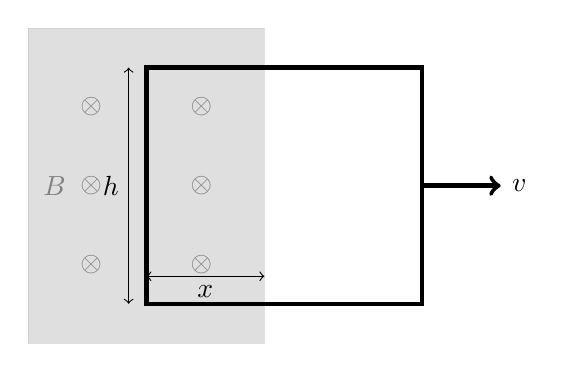
\begin{tikzpicture}
            \tikzstyle{magnetic field} = [color=lightgray, fill=lightgray, draw opacity=0.5, fill opacity=0.5]
            \tikzstyle{magnetic field label} = [color=gray]
            \tikzstyle{line} = [ultra thick]
            \draw[magnetic field] (0, 0) rectangle (3, 4);
            \foreach \x in {0.8, 2.2} {
                \foreach \y in {1, 2, 3} {
                    \node[magnetic field label] at (\x, \y) {\(\otimes\)};
                }
            }
            \node[magnetic field label, left] at (0.6, 2) {\(\vv{B}\)};
            \draw[line] (1.5, 0.5) rectangle (5, 3.5);
            \draw[line, ->] (5, 2) -- (6, 2) node[right] {\(\vv{v}\)};
            \draw[<->] (1.275, 0.5) -- (1.275, 3.5) node[midway, left] {\(h\)};
            \draw[<->] (1.5, 0.85) -- (3, 0.85) node[midway, below] {\(x\)};
        \end{tikzpicture}
        \caption{Wire loop moving through a magnetic field inducing an \gls{emf}.}
        \label{fig:induced emf in a loop moving through a magnetic field}
    \end{figure}
    The loop is dragged out of the field with a velocity \(\vv{v}\).
    The force on a charge carrier in the loop due to the magnetic field is given by
    \[\vv{F_M} = q\vv{v}\times\vv{B}.\]
    The \gls{emf} is
    \[\emf = \oint\vv{F_M}\cdot\dd{\vv{l}} = hvB.\]
    Here we have used that the force along the top and bottom parts of the loop are in opposite directions so cancel, meaning we only need to consider the contribution to the \gls{emf} of the force along the vertical section in the field.
    
    We can also calculate the magnetic flux:
    \[\Phi_B = \int\vv{B}\cdot\dd{\vv{S}} = Bhx\]
    where we define the surface normal so that the right hand rule with the current direction is satisfied.
    The flux is clearly not constant as the area of the loop that is in the field is changing:
    \[\dv{\Phi_B}{t} = \dv{t}Bhx = Bh\dv{x}{t} = -Bhx = -\emf.\]
    Note the minus sign as the area is decreasing.
    In fact the statement,
    \[\emf = -\dv{\Phi_B}{t},\]
    holds in general.
    This is called \define{Faraday's law of induction}.
    We say that this \gls{emf} is an induced \gls{emf} as it doesn't come from a normal source of \gls{emf} but rather the interaction of electric and magnetic fields.
    
    \subsection{Faraday's Law}
    Experimentally Faraday showed that altering \(\Phi_B\) by any of the following:
    \begin{enumerate}
        \item moving the surface,
        \item moving the field region,
        \item varying the field strength,
    \end{enumerate}
    produced an induced \gls{emf} in accordance with Faraday's law of induction.
    
    Note that in the last two of these the charges don't move so \(\vv{v} = 0\) meaning \(\vv{F_M} = \vv{0}\).
    Assuming that the Lorentz force law is correct there must be an induced electric field which creates a current.
    
    Faraday;s law has a differential form:
    \[\emf = -\dv{\Phi_B}{t} \implies \oint_C\vv{E}\cdot\dd{\vv{l}} = -\dv{t}\int_S\vv{B}\cdot\dd{\vv{S}}.\]
    Here \(C\) is the loop, \(S\) is the surface it encloses, and we have simply replaced \(\emf\) and \(\Phi_B\) with their definitions.
    We assume that the surface is constant so
    \[\dv{t}\int_S\vv{B}\cdot\dd{\vv{S}} = \int_S\partial_t\vv{B}\cdot\dd{\vv{S}}.\]
    We can also use Stokes' law to get
    \[\oint_C\vv{E}\cdot\dd{\vv{l}} = \int_S\curl\vv{E}\cdot\dd{\vv{S}}.\]
    Hence
    \[\int_S\curl\vv{E}\cdot\dd{\vv{S}} = -\int_S\partial_t\vv{B}\cdot\dd{\vv{S}}.\]
    Since both integrals are over the same area we must have that
    \[\curl\vv{E} = -\partial_t.\]
    We see that \(\curl\vv{E} = \vv{0}\) only holds for static magnetic fields.
    This is the full version of this law and is Maxwell's third equation.
    \[\emf = \oint_C\vv{E}\cdot\dd{\vv{l}} = -\dv{\Phi_B}{t} = -\dv{t}\int_S\vv{B}\cdot\dd{\vv{S}} \iff \curl\vv{E} = -\partial_t\vv{B}. \tag{MIII}\]
    
    \subsection{Connection to the Magnetic Vector Potential}
    If we combine \(\curl\vv{E} = -\partial_t\vv{B}\) and \(\vv{B} = \curl\vv{A}\) then we have
    \[\curl\vv{E} = -\partial_t(\curl\vv{A}) = -\curl(\partial_t\vv{A})\]
    which means
    \[\curl(\vv{E} - \partial_t\vv{A}) = \vv{0}.\]
    This means that there must exist a scalar field, \(V\), such that
    \[\vv{E} - \partial_t = -\grad V.\]
    Rearranging this we have
    \[\vv{E} = -\grad V - \partial_t\vv{A}.\]
    This is the most general way to write \(\vv{E}\) in terms of potentials, it reduces to \(\vv{E} = -\grad V\) if \(\vv{B}\) is time independent.
    We have now fixed the two equations that we showed weren't correct in section~\ref{sec:sources of steady current}.
    We see that there are two sources of the electric field:
    \begin{itemize}
        \item A stationary charge distribution, \(\rho\), which gives a contribution \(-\grad V\).
        \item A time dependent magnetic field, \(\vv{B}\), which gives a contribution \(-\partial_t\vv{A}\).
    \end{itemize}

    \subsection{Lenz's Law}
    \define{Lenz's law} is a rule of thumb that allows us to decide the sign of the flux.
    It states that the induced \gls{emf}, \(\emf\), acts in a way as to oppose the change that created it.
    For example in the case of removing a wire from a magnetic field the \gls{emf} causes a current in the wire in a direction such that the force due to the magnetic field's interaction with this current is in the opposite direction to the direction which the wire is being pulled.
    This is useful as it is often not that easy to see what the direction of the flux is and hence the direction of the induced \gls{emf} and induced current.
    
    \section{Induction}
    \subsection{Induction Examples}
    \subsubsection{AC Generator}
    A current loop, initially the \((x, z)\)-plane, with area \(A\) is placed in a uniform magnetic field, \(\vv{B}\).
    The loop is rotated at an angular velocity \(\vv{\omega} = \omega\ve{z}\).
    Since the loop is rotating the flux through the loop is time dependent:
    \[\Phi_B = \int_A\vv{B}\cdot\dd{\vv{S}} = B\cos(\omega t)\int_A\dd{S} = AB\cos(\omega t).\]
    Therefore there is an induced \gls{emf}:
    \[\emf = -\dv{\Phi_B}{t} = AB\omega\sin(\omega t).\]
    The induced current will be an AC current with a frequency \(\omega\).
    The current is \(\pi/2\) out of phase with the flux in a way that means that the peak current occurs when the flux is zero.
    
    \subsubsection{Rotating Disc of Charge}
    An insulating disc of radius \(a\) with a uniform surface charge density, \(\sigma\), is rotated around its axis.
    There is a uniform magnetic field parallel to the axis of the disc.
    The magnetic force on a charge element, \(\dd{q}\), on the disc at a radius \(r\), is
    \[\dd{\vv{F}} = \dd{q}vB\ve{\rho} = \dd{q}r\omega B\ve{\rho}.\]
    This magnetic force is equivalent to a radial electric field:
    \[\vv{E'} = \frac{1}{q}\vv{F} = r\omega B\ve{\rho}.\]
    The induced \gls{emf} between the centre and edge of the disc is then
    \[\emf = \int_{0}^a\vv{E'}\cdot\ve{\rho}\dd{\rho} = \frac{\omega Ba^2}{2}.\]
    This acts outwards to move the charge to the outside of the disc.
    If the disc were a conductor then this would actually happen.
    
    While the flux rule,
    \[\emf = -\dv{\Phi_B}{t},\]
    is still valid there is not a useful current loop to compute the flux through so it isn't of much help in this problem.
    
    \subsection{Mutual Inductance}
    Two current loops, \(C_1\) and \(C_2\) are carrying currents \(I_1\) and \(I_2\) in directions \(\dd{\vv{l_1}}\) and \(\dd{\vv{l_2}}\) respectively at positions \(\vv{r_1}\) and \(\vv{r_2}\).
    Current \(I_1\) creates a magnetic field, \(\vv{B_1}\), which passes through loop 2.
    Therefore a current is induced in loop 2.
    The induced flux in loop 2 is
    \[\Phi_2 = \int_{S_2}\vv{B_1}\cdot\dd{\vv{S_2}} = M_{21}I_1\]
    where we have used that \(\abs{\vv{B_1}}\propto I_1\) and \(M_{21}\) is just a constant of proportionality called the \define{mutual inductance}.
    If we substitute the vector potential, \(\vv{A_1}\), such that \(\vv{B_1} = \curl\vv{A_1}\), we get
    \begin{align*}
        \Phi_2 &= \int_{S_2} \vv{B_1}\cdot\dd{\vv{S_2}}\\
        &= \int_{S_2} (\curl\vv{A_1})\cdot\dd{\vv{S_2}}\\
        &= \oint_{C_2} \vv{A_1}\cdot\dd{\vv{l_1}}\\
        &= \frac{\mu_0 I_1}{4\pi} \oint_{C_2}\oint_{C_1} \frac{\dd{\vv{l_1}}\cdot\dd{\vv{l_2}}}{\abs{\vv{r_1} - \vv{r_2}}}.
    \end{align*}
    In the last step we have used the explicit solution to \gls{pe}, \(\laplacian\vv{A} = -\mu_0\vv{J}\).
    This gives us that
    \[M_{21} = \frac{\mu_0}{4\pi}\oint_{C_2}\oint_{C_1} \frac{\dd{\vv{l_1}}\cdot\dd{\vv{l_2}}}{\abs{\vv{r_1} - \vv{r_2}}}.\]
    This is called the Neumann formula.
    It isn't that useful, as it is pretty hard to calculate for arbitrary geometries, it is important to note that it is symmetric in 1 and 2, that is if we perform the equivalent calculation but completely swap the two loops we will get the same answer so
    \[M_{21} = M_{12} = M.\]
    The flux through loop 1 due to a current \(I\) in loop 2 is the same as the flux through loop 2 due to a current \(I\) in loop 1.
    
    The induced \gls{emf} in loop 2 due to current \(I_2\) is
    \[\emf_2 = -\dv{\Phi_2}{t} = -\dv{t}[MI_1] = -M\dv{I_1}{t}.\]
    We can then use Lenz's law to calculate the direction of the current noting that it must oppose any change in \(I_1\).
    
    One application of this is a spark plug in a car.
    In this loop 1 is wrapped around a core a few times and loop 2 is wrapped around the same core many many times.
    This leads to a very large value of \(M\) and so a small current in loop 1 can create a very large current in loop 2 which is large enough to spark across an air gap and ignite the fuel.
    
    \subsection{Self Inductance}
    If a loop carries a current then it generates a magnetic field.
    This magnetic field creates a flux through the loop.
    Therefore if the current is time dependent there will be an induced \gls{emf} and induced current in the loop that acts to oppose the change in the initial current.
    The \gls{emf} will be
    \[\emf = -\dv{\Phi_B}{t} = -L\dv{I}{t},\]
    where we have defined \(L\), the \define{self inductance}, to be such that \(\Phi_B = LI\).
    
    For example a solenoid of length \(\ell\) and radius \(a\) with \(n\) loops per unit length has an interior magnetic field of
    \[\vv{B} = B_z\ve{z} = \mu_0 nI\ve{z}.\]
    Each loop is approximately a closed circle of area \(A = \pi a^2\) and so the total flux through all \(n\ell\) loops is
    \[\Phi_B = \int \vv{B}\cdot\dd{\vv{S}} = An\ell B_z = \mu_0I\pi a^2n^2\ell.\]
    We can then identify the self inductance as
    \[L = \mu_0 \pi a^2n^2\ell = \mu_0n^2V_s\]
    where \(V_s = \pi a^2\ell\) is the volume of the solenoid.
    
    \subsection{Electronics}
    \textit{This section is non-examinable}
    
    We have introduced three material properties which all relate a voltage, \(\Delta V\), to the charge, \(Q\), in a different way:
    \begin{itemize}
        \item Resistance, \(R\):
        \[\Delta V \sim I \sim \dv{Q}{t}.\]
        \item Capacitance, \(C\):
        \[\Delta V\sim Q.\]
        \item Inductance, \(L\):
        \[\Delta V \sim \dv{I}{t} \sim \dv[2]{Q}{t}.\]
    \end{itemize}
    By constructing a circuit with two of these in series we can model differential equations.
    Since they are in series the voltage in all components will be the same.
    We start with a resistor and capacitor.
    From the fact that the voltages are equal we have that
    \[\dv{Q}{t} \sim Q \implies Q = Q_0e^{-\alpha t}\]
    for some constants \(Q_0\) and \(\alpha\).
    If we swap the capacitor for an inductor then we will have
    \[\dv{I}{t} \sim I \implies I = I_0e^{-\beta t}\]
    for some constants \(I_0\) and \(\beta\).
    Finally if we have a capacitor and inductor in series then
    \[\dv[2]{Q}{t} \sim Q \implies Q = Q_0'\sin(\omega t + \varphi) \implies I = Q_0'\omega\cos(\omega t + \varphi)\]
    for some constants \(Q_0'\), \(\omega\), and \(\varphi\).
    
    In the first case the charge on the capacitor decays away exponentially.
    In the second case the current that is initially induced by the inductor decays away exponentially.
    In the last case if initially we start with a charged capacitor and with no current (\(\varphi = \pi/2\)) then as the capacitor discharges a current is is induced and this charges the capacitor and we get an oscillating charge and current.
    
    \subsection{Magnetic Energy in Inductors}\label{sec:energy magnetic field}
    In electrostatics the electrostatic energy is due to the work done to create a charge distribution, done against Coulomb repulsion.
    Similarly in magnetostatics the magnetostatic energy is due to the work done to create a steady current, done against the induced \gls{emf} which opposes the creation of any current.
    
    If we try to create a current, \(\dd{I}\), in a loop in time \(\dd{t}\) we need to do work against the induced \gls{emf}, \(\emf\):
    \[\dd{U_M} = -\emf I\dd{t} = LI\dv{I}{t}\dd{t} = LI\dd{I},\]
    where \(L\) is the self inductance of the loop and we have used that
    \[-\emf = \dv{\Phi_B}{t} = \dv{t}[LI] = LI\dv{I}{t}.\]
    Integrating the energy with time we get
    \[U_M = \frac{1}{2}LI^2.\]
    Compare this to the equivalent statement in electrostatics that
    \[U_E = \frac{1}{2}\frac{Q^2}{C}.\]
    For two loops with inductances \(L_1\) and \(L_2\) carrying currents \(I_1\) and \(I_2\) with mutual inductance \(M\) then the energy becomes
    \[U_M = \frac{1}{2}L_1I_1^2 + \frac{1}{2}L_2I_2^2 + MI_1I_2.\]
    We can generalise the energy to any current arrangement:
    \begin{align*}
        U_M = \frac{1}{2}LI^2\\
        &= \frac{1}{2}\Phi_BI\\
        &= \frac{1}{2}I\oint_C \vv{A}\cdot\dd{\vv{l}}\\
        &= \frac{1}{2}\oint_C \vv{A}\cdot\vv{I}
    \end{align*}
    for a single loop.
    Notice that \(\oint_C \vv{A}\cdot\vv{I}\) is effectively a volume integral over all space of \(\vv{J}\) since this is only non-zero where there is a current, which in the case of a single loop reduces to a contour integral.
    Hence
    \[U_M = \frac{1}{2}\int\vv{A}\cdot\vv{J}\dd{V}.\]
    Where the integral is performed over all space.
    Using Amp\`ere's law we have
    \begin{align*}
        \mu_0\vv{A}\cdot\vv{J} &= \vv{A}\cdot(\curl\vv{B})\\
        &= \abs{\vv{B}}^2 - \div(\vv{A}\times\vv{B})
    \end{align*}
    where we have used the vector identity
    \begin{align*}
        \div(\vv{A}\times\vv{B}) &= \vv{B}\cdot\underbrace{(\curl\vv{A})}_{=\vv{B}} - \vv{A}\cdot(\curl\vv{B})\\
        &= \vv{B}\cdot\vv{B} - \vv{A}\cdot(\curl\vv{B})\\
        &= \abs{\vv{B}}^2 - \vv{A}\cdot(\curl\vv{B}).
    \end{align*}
    Hence the energy is
    \[U_M = \frac{1}{2}\vv{A}\cdot\vv{J}\dd{V} = \frac{1}{2\mu_0}\int\abs{\vv{B}}^2\dd{V} - \frac{1}{2\mu_0}\int\div(\vv{A}\times\vv{B})\dd{V}.\]
    We can write this last integral as a surface integral using the divergence theorem:
    \[\int\div(\vv{A}\times\vv{B})\dd{V} = \oint_S(\vv{A}\times\vv{B})\cdot\dd{\vv{S}}.\]
    If \(A\sim 1/r\) and \(B\sim 1/r^2\), as is the case for steady, finite, localised currents, then \(\abs{\vv{A}\times\vv{B}}\sim 1/r^3\).
    The surface area, \(S\sim r^2\).
    Since the volume integral is over all space the surface integral is over a boundary at infinity and so
    \[\int(\vv{A}\times\vv{B})\cdot\dd{\vv{S}} \sim \frac{1}{r^3}r^2 = \frac{1}{r}\]
    which becomes zero as \(r\to\infty\).
    Hence the energy is
    \[U_M = \frac{1}{2\mu_0}\int\abs{\vv{B}}^2\dd{V}.\]
    We can define an energy density, \(u_M\), such that
    \[u_m = \frac{\abs{\vv{B}}^2}{2\mu_0} \implies U_M = \int u_m\dd{V}.\]
    Compare this to the electrostatic case
    \[u_E = \frac{1}{2}\varepsilon\abs{\vv{E}}^2.\]
    
    \section{Displacement Current}
    \subsection{The Continuity Equation}
    The global electric charge is conserved.
    This means that the only way that the charge contained in a volume, \(V\), can change is if charge enters or leaves the volume.
    In the case that this happens there will be a current \(\vv{J}\) associated with the charge moving.
    The charge enters the volume at a rate of
    \[\pdv{Q}{t} = -\oint_S\vv{J}\cdot\dd{\vv{S}}.\]
    The minus sign accounts for the fact the surface normal, \(\dd{\vv{S}}\), points out of the volume so \(\vv{J}\cdot\dd{\vv{S}}\) is the charge leaving the volume through the surface \(\dd{\vv{S}}\), on the other hand \(\partial_t\) is the rate of increase of charge.
    Substituting in the charge density and applying the divergence theorem we have
    \[-\pdv{t}\int_{V}\rho\dd{V} = \int_V \div\vv{J}\dd{V}.\]
    Since this holds for all volumes we must have
    \[-\pdv{\rho}{t} = -\div\vv{J}.\]
    This is the \define{continuity equation}.
    It actually applies to any conserved quantity with an associated density and current.
    For example if \(\rho\) is mass density and \(\vv{J}\) is mass current which describes how mass is moving, for example it may describe fluid flow, then the continuity equation applies.
    Another important application is in quantum mechanics where \(\rho\) is the probability density and \(\vv{J}\) is a probability current which describes how the probability of different states changes with time.
    
    \subsection{Displacement Current}
    Amp\`ere's law is
    \[\curl\vv{B} = \mu_0\vv{J}.\]
    Taking the divergence of this we have
    \[\div(\curl\vv{B}) = \mu_0\div\vv{J}.\]
    The left hand side is identically zero by a vector calculus identity.
    For the right hand side we apply the continuity equation and get
    \[0 = -\mu_0\pdv{\rho}{t}.\]
    This is obviously wrong for a non-static charge distribution, \(\rho(\vv{r}, t)\), which we know can exist and would expect \(\rho\) not to be constant with time.
    Using the continuity equation we can known
    \[\div\vv{J} + \pdv{\rho}{t} = 0\]
    and so
    \[\div(\curl\vv{B}) = \mu_0(\div\vv{J} + \partial_t\rho)\]
    From Maxwell's first law we know that
    \[\rho = \varepsilon_0\div\vv{E}\]
    so
    \[\div(\curl\vv{B}) = \mu_0(\div\vv{J} + \varepsilon_0\partial_t\div\vv{E}) = \mu_0 \div(\vv{J} + \varepsilon_0\partial_t\vv{E})\]
    Since \(\div(\curl\vv{K}) = 0\) for all vector fields, \(\vv{K}\), we must have
    \[\curl\vv{B} = \mu_0(\vv{J} + \varepsilon_0\partial_t\vv{E} + \curl\vv{K}).\]
    It turns out that \(\vv{K} = \vv{0}\), this is required so that in the static case this equation reduces to \(\curl\vv{B} = \mu_0\vv{J}\).
    Therefore
    \[\curl\vv{B} = \mu_0(\vv{J} + \varepsilon_0\partial_t\vv{E}).\]
    This is the \define{Amp\`ere--Maxwell law} and is the full version of Maxwell's fourth equation with time dependent fields.
    It also has an integral form, using Stoke's theorem we have
    \[\int_S(\curl\vv{B})\cdot\dd{\vv{S}} = \oint_C \vv{B}\cdot\dd{\vv{l}}\]
    also
    \[\mu_0\int_S \vv{J}\cdot\dd{\vv{S}} + \varepsilon_0\int_S \pdv{t}\vv{E}\cdot\dd{\vv{S}} = \mu_0\int_S \vv{J}\cdot\dd{\vv{S}} + \mu_0\varepsilon_0\dv{t}\int\vv{E}\cdot\dd{\vv{S}}\]
    so
    \[\oint_C\vv{B}\cdot\dd{\vv{l}} = \mu_0\int_S \vv{J}\cdot\dd{\vv{S}} + \mu_0\varepsilon_0\dv{t}\int\vv{E}\cdot\dd{\vv{S}}\]
    What this law tells us is that magnetic fields can originate from two sources:
    \begin{itemize}
        \item Steady currents, \(\vv{J}\)
        \item Time dependent electric fields, \(\vv{E}\) (which themselves are created by time dependent charge densities or time dependent magnetic fields that change at a non-constant rate).
    \end{itemize}
    We call \(\varepsilon_0\partial_{t}\vv{E}\) the \define{displacement current} because it has dimensions of current density and creates a magnetic field.
    It is not a real current however.
    
    \subsubsection{Capacitor Paradox and Resolution}
    The capacitor paradox is another example of why Amp\`ere's law alone is not quite correct.
    The capacitor paradox is as follows.
    Consider a capacitor charging/discharging with a time dependent current, \(I(t)\),
    What is the magnetic field?
    Since the current is time dependent then so is the field.
    By Amp\`ere's law we have
    \[\oint_C\vv{B}\cdot\dd{\vv{l}} = \mu_0\int_S\vv{J}\cdot\dd{\vv{S}}.\]
    The paradox arises in the right hand side of this equation.
    If we take the surface \(S\) to cut through the wire then the right hand side is equal to \(\mu_0I(t)\).
    It is also possible to construct a surface with the same boundary in a way such that the surface goes in between the plates of the capacitor without ever intersecting any of the circuit.
    Then the right hand side of this equation is zero.
    
    We fix the supposed paradox by using the full Amp\`ere--Maxwell law.
    We known that for an ideal parallel plate capacitor the electric field is entirely constrained to be between the plates and in this volume it is normal to the plates and the field strength is
    \[E(t) = \frac{Q(t)}{\varepsilon_0 A}\]
    where \(A\) is the area of the plates.
    If we define the direction of \(\vv{E}\) to be the \(z\) direction then
    \[\varepsilon_0\partial_t\vv{E} = \frac{1}{A}\pdv{Q}{t}\ve{z} = \frac{I(t)}{A}\ve{z}.\]
    If we also choose to construct the surface so that it is parallel to the plates of the capacitor when it is between them then
    \[\mu_0\int_{S_2}(\vv{J} + \varepsilon_0\partial_t\vv{E})\cdot\dd{\vv{S}} = \frac{I(t)}{A}\int_{S_2}\dd{S} = \mu_0I(t)\]
    where we have used the fact that the field is zero outside of the capacitors so the surface integral is equivalent to an integral over the area of the capacitor.
    This is exactly the same result that we get using the other surface so we have fixed the paradox.
    \begin{figure}[ht]
        \centering
        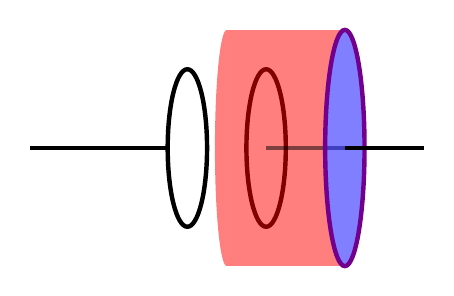
\begin{tikzpicture}
            \tikzstyle{line} = [ultra thick]
            \draw[line] (0, 0) -- (1.75, 0);
            \draw[line] (2, 0) circle[x radius=0.25cm, y radius=1cm];
            \draw[line] (3, 0) circle[x radius=0.25cm, y radius=1cm];
            \fill[color=red, opacity=0.5] (2.5, -1.5) rectangle (4, 1.5);
            \begin{scope}
                \clip (2.5, -1.5) rectangle (0, 1.5);
                \fill[color=red, opacity=0.5] (2.5, 0) circle[x radius=0.15cm, y radius=1.5cm];
            \end{scope}
            \draw[color=red, opacity=0.25] (2.5, -1.5) -- (2.5, 1.5);
            \fill[white] (4, 0) circle[x radius=0.25cm, y radius=1.5cm];
            \draw[line, opacity=0.5] (3, 0) -- (5, 0);
            \fill[color=blue, opacity=0.5] (4, 0) circle[x radius=0.25cm, y radius=1.5cm];
            \draw[color=red!45!blue, line] (4, 0) circle[x radius=0.25cm, y radius=1.5cm];
            \draw[line] (4, 0) -- (5, 0);
        \end{tikzpicture}
        \caption{The capacitor paradox. The two surfaces used in the capacitor paradox. \(S_1\) in blue goes through the wire and \(S_2\) in red goes through the gap in the capacitor. They share the boundary, \(C\), shown in purple.}
    \end{figure}
    
    \subsection{Maxwell's Equations}
    Maxwell's equations in differential form are
    \begin{align*}
        \div \vv{E} &= \frac{\rho}{\varepsilon_0},\tag{MI}\\
        \div \vv{B} &= 0,\tag{MII}\\
        \curl\vv{E} &= -\partial_t\vv{B},\tag{MIII}\\
        \curl\vv{B} &= \mu_0(\vv{J} + \varepsilon_0\partial_t\vv{E}).\tag{MIV}\\
    \end{align*}
    In integral form these are
    \begin{align*}
        \oint_S \vv{E}\cdot\dd{\vv{S}} &= \frac{Q_\enc}{\varepsilon_0}, \tag{MI}\\
        \oint_S \vv{B}\cdot\dd{\vv{S}} &= 0, \tag{MII}\\
        \oint_C \vv{E}\cdot\dd{\vv{l}} &= -\dv{t}\int_S \vv{B}\cdot\dd{\vv{S}} = -\dv{\Phi_B}{t} = \emf, \tag{MIII}\\
        \oint_C \vv{B}\cdot\dd{\vv{l}} &= \mu_0\int_S\vv{J}\cdot\dd{\vv{S}} + \mu_0\varepsilon_0\dv{t}\int_S \vv{E}\cdot\dd{\vv{S}} = \mu_0I_{\enc} + \mu_0\varepsilon_0\dv{\Phi_E}{t}. \tag{MIV}
    \end{align*}
    The first two equations are Gauss' laws for electric and magnetic fields, the third is Faraday's law of induction and the fourth is the Amp\`ere--Maxwell law.
    Combining Maxwell's first and fourth laws as well as the fact that the divergence of a curl is zero we get
    \[0 = \div(\curl\vv{B}) = \mu_0\left[\div\vv{J} + \varepsilon_0 \partial_t\div\vv{E} \right] = \mu_0\left[\div\vv{J} + \partial_t\rho\right]\]
    which is the continuity equation again.
    \subsubsection{Solutions to Maxwell's Equation}
    We will look for non-trivial solutions to Maxwell's equations in free space, that is with \(\rho = 0\) and \(\vv{J} = \vv{0}\).
    In this case Maxwell's equations become
    \begin{align*}
        \div\vv{E} &= 0\tag{MI in free space}\\
        \div\vv{B} &= 0\tag{MII}\\
        \curl\vv{E} &= -\partial_t\vv{B}\tag{MIII}\\
        \curl\vv{B} &= \mu_0\varepsilon_0\partial_t\vv{E}\tag{MIV in free space}
    \end{align*}
    Taking the curl of the third equation we have
    \[\curl(\curl\vv{E}) = -\curl(\partial_t\vv{B}) = -\partial_t\curl\vv{B} = -\mu_0\varepsilon_0\partial_t^2\vv{E}.\]
    Similarly taking the curl of the fourth equation we have
    \[\curl(\curl\vv{B}) = \mu_0\varepsilon_0\curl(\partial_t\vv{E}) = \mu_0\varepsilon_0\partial_t\curl\vv{E} = -\mu_0\varepsilon_0\partial_t^2\vv{B}.\]
    Or we can use the vector identity
    \[\curl(\curl\vv{K}) = \grad(\div\vv{K}) - \laplacian\vv{K}\]
    and we get
    \[\curl(\curl\vv{E}) = \grad(\div\vv{E}) - \laplacian\vv{E} = -\laplacian\vv{E},\]
    and
    \[\curl(\curl\vv{B}) = \grad(\div\vv{B})  -\laplacian\vv{B} = -\laplacian\vv{E}.\]
    Thus
    \[\partial_t^2\vv{E} = \frac{1}{\mu_0\varepsilon_0}\laplacian\vv{E}\qquad\text{and}\qquad \partial_t^2\vv{B} = \frac{1}{\mu_0\varepsilon_0}\laplacian\vv{B}.\]
    Thus we have turned four coupled first order \glspl{pde} into two seemingly uncoupled second order \glspl{pde}.
    They are only seemingly uncoupled as Maxwell's laws always apply.
    We can identify these equations as wave equations, which have the general form
    \[\partial_t^2\vv{u} = v^2\laplacian\vv{u}\]
    where \(v\) is the speed of waves in the vector field \(\vv{u}\).
    We see that for the waves in the electric and magnetic fields
    \[v = \frac{1}{\sqrt{\mu_0\varepsilon_0}} = c\]
    and indeed these equations relate to electromagnetic waves.
    
    \section{Electromagnetic Waves}
    \subsection{The Wave Equation in One Dimension}
    The wave equation for a scalar field, \(u\), with a wave propagating at speed \(c\), is
    \[\pdv[2]{u}{x} = \frac{1}{c^2}\pdv[2]{u}{t}.\]
    This is a second order \gls{pde} and typically we have initial conditions of \(u(x, 0)\) and \(\dot{u}(x, 0)\).
    Any twice differentiable function, \(u\), of the form
    \[u(x, t) = f(kx - \omega t),\]
    or equivalently
    \[u(x, t) = g(x - ct),\]
    satisfies this equation and represents a wave moving in the \(x\) direction at speed
    \[c = \frac{\omega}{k},\]
    with frequency \(\omega\) and wave number \(k\).
    For example,
    \[u(x, t) = u_0\exp\left[-\frac{(x - ct)^2}{2\sigma^2}\right]\]
    describes a Gaussian wave packet moving in the \(x\) direction at speed \(c\).
    The most important function of this form is
    \[u(x, t) = A\exp[i(kx - \omega t)] = A\cos(kx - \omega t) + iA\sin(kx - \omega t).\]
    Here \(A\) is the amplitude of the waves (it is possible that this is complex).
    We can see that this is made of two sinusoidal waves which are independent of each other.
    This wave, \(u\), is monochromatic because, although it is a superposition of two waves, both have the same frequency, \(\omega\).
    Sine and cosine form a basis for a Fourier expansion of some arbitrary solution, \(u(x, t)\).
    By this we mean that given a solution, \(u\), to the wave equation it is always possible to write it as a superposition of sinusoids.
    It is often convenient to work with complex expressions and then take the real part when we need to get a physical solution.
    For example,
    \begin{align*}
        u(x, t) &= \Re[A\exp(i(kx - \omega t))]\\
        &= \Re[A\cos(kx - \omega t) + iA\sin(kx - \omega t)]\\
        &= \Re[A\cos(kx - \omega t)] + \Im[A\sin(kx - \omega t)].
    \end{align*}
    Here we have used that if \(z = a + bi\) for \(a, b\in\reals\) then 
    \[\Re[iz] = \Re[ia] - \Re[b] = -b.\]
    To solve the wave equation we start by writing the initial conditions as inverse Fourier transforms:
    \[u(x, 0) = \int_{-\infty}^{\infty} \tilde{g}(k)e^{ikx}\dd{k}\]
    and
    \[\dot{u}(x, 0) = \int_{-\infty}^{\infty} \tilde{h}(k)e^{ikx}\dd{k}\]
    where \(g(x) = u(x, 0)\) and \(h(x) = \dot{u}(x, 0)\) and \(\tilde{g}\) and \(\tilde{h}\) are the Fourier transforms of \(g\) and \(h\) respectively.
    We then solve the wave equation for the initial conditions
    \[f(x, 0) = \tilde{g}(k)e^{ikx},\qquad\text{and}\qquad \dot{f}(x, 0) = \tilde{h}(k)e^{ikx}.\]
    We obtain the monochromatic solution
    \[f(kx - \omega t) = \left[\tilde{g}(k) + \frac{i}{\omega}\tilde{h}(k)\right]\exp[i(kx - \omega t)].\]
    The full solution, \(u = u(x, t)\), is then a superposition of all frequencies/wave numbers which we can write as an integral over one of these:
    \[u(x, t) = \int_{-\infty}^{\infty} f(kx - \omega t)\dd{k} = \int_{-\infty}^{\infty} \left[\tilde{g}(k) + \frac{i}{\omega}\tilde{h}(k)\right]\exp[i(kx - \omega t)]\dd{k}.\]
    
    \subsection{The Wave Equation in Three Dimensions}
    In three dimensions the wave equation for a scalar field, \(u\), with a wave propagating at speed \(c\), is
    \[\laplacian u = \frac{1}{c^2}\pdv[2]{u}{t}.\]
    Again any twice differentiable function of the form
    \[u(\vv{r}, t) = f(\vv{k}\cdot\vv{r} - \omega t)\]
    is a solution.
    Here \(\vv{k}\) is the wave vector which points in the direction of propagation and is such that \(c = \omega / k\) still.
    A similar form that is still a solution is
    \[u(\vv{r}, t) = g(\vh{k}\cdot\vv{r} - ct).\]
    We will show here that a plane wave,
    \[u(\vv{r}, t) = A\exp[i(\vv{k}\cdot\vv{r} - \omega t)],\]
    is a solution.
    \begin{align*}
        \grad u(\vv{r}, t) &= \grad A\exp[i(\vv{k}\cdot\vv{r} - \omega t)]\\
        &= \ve{j}\partial_j A\exp[i(k_jx_j - \omega t)]\\
        &= \ve{j}k_jk A\exp[i(k_jx_j - \omega t)]\\
        &= i\vv{k} A\exp[i(\vv{k}\cdot\vv{r} - \omega t)]\\
        &= i\vv{k} u(\vv{r}, t).
    \end{align*}
    We see here the reason that this is called a plane wave.
    The gradient gives the direction of fastest increase and in this case \(\grad u\) is parallel to \(\vv{k}\).
    This means that in a plane normal to \(\vv{k}\), that is for the plane
    \[\vv{k}\cdot\vv{r} = \omega t + a,\]
    for some \(a\in\reals\), \(u(\vv{r}, t)\) has the same value everywhere in the plane.
    Continuing on with showing that this is indeed a wave:
    \begin{align*}
        \laplacian u(\vv{r}, t) &= \div\grad u(\vv{r}, t)\\
        &= \div [i\vv{k}u(\vv{r}, t)]\\
        &= i\vv{k}\cdot\grad u(\vv{r}, t)\\
        &= i\vv{k}\cdot i\vv{k}u(\vv{r}, t)\\
        &= -k^2u(\vv{r}, t).
    \end{align*}
    Also
    \begin{align*}
        \frac{1}{c^2}\pdv[2]{t}u(\vv{r}, t) &= \frac{1}{c^2}\pdv[2]{t}A\exp[i(\vv{k}\cdot\vv{r} - \omega t)]\\
        &= -\frac{1}{c^2}\omega^2A\exp[i(\vv{k}\cdot\vv{r} - \omega t)]\\
        &= -\frac{\omega^2}{c^2}u(\vv{r}, t)
    \end{align*}
    so we see that \(u\) is a solution as long as \(k = \omega/c\).
    
    \subsection{The Wave Equation for a Vector Field}
    The wave equation for a vector field, \(\vv{F}\), is
    \[\laplacian\vv{F}(\vv{r}, t) = \frac{1}{c^2}\pdv[2]{t}\vv{F}(\vv{r}, t).\]
    This has the expected plane wave solution:
    \[\vv{F}(\vv{r}, t) = \vv{F_0}\exp[i(\vv{k}\cdot\vv{r} - \omega t)].\]
    Here \(\vv{F_0}\) is a constant (possibly complex) vector.
    In a similar way to the previous section we can show that for a plane wave \(\vv{F}(\vv{r}, t)\)
    \[\div\vv{F} = i\vv{k}\cdot\vv{F}, \qquad\text{and}\qquad \laplacian\vv{F} = -k^2\vv{F}.\]
    We also have that
    \[\curl\vv{F} = i\vv{k}\times\vv{F}.\]
    
    \subsection{Electromagnetic Plane Waves}
    The wave equations for the electric and magnetic fields in free space are
    \[\laplacian\vv{E} = \mu_0\varepsilon_0\pdv[2]{t}\vv{E}, \qquad\text{and}\qquad \laplacian\vv{B} = \mu_0\varepsilon_0 \pdv[2]{t}\vv{B}.\]
    The plane wave solutions to these are
    \[\vv{E} = \vv{E_0}\exp[i(\vv{k}\cdot\vv{r} - \omega t)], \qquad\text{and}\qquad \vv{B} = \vv{B_0}\exp[i(\vv{k}\cdot\vv{r} - \omega t)].\]
    In free space we know that \(\div\vv{E} = \div\vv{B} = 0\).
    We also know the divergence of a plane wave, \(\vv{F}\), is \(\div\vv{F} = i\vv{k}\cdot\vv{F}\), so we must have
    \[0 = i\vv{k}\cdot\vv{E}.\]
    This implies that \(\vv{k}\cdot\vv{E} = 0\) which means that \(\vv{k}\) and \(\vv{E}\) are perpendicular.
    The exact same logic shows us that \(\vv{k}\) and \(\vv{B}\) must be perpendicular.
    For this reason we call electromagnetic waves transverse because their amplitude is in a plane perpendicular to the direction of propagation, which is along \(\vv{k}\).
    
    Maxwell's third law in free space gives us \(\curl\vv{E} = -\partial_t\vv{B}\).
    We also know that the curl of a plane wave, \(\vv{F}\), is \(\curl\vv{F} = i\vv{k}\times\vv{F}\), and the time derivative of a plane wave, \(\vv{F}\), is \(\partial_t\vv{F} = -i\omega\vv{F}\).
    Thus
    \[-i\omega\vv{B} = i\vv{k}\times\vv{E}.\]
    This means that \(\vv{B}\) and \(\vv{E}\) are perpendicular, further
    \[E = \frac{\omega}{k}B = cB.\]
    So not only are \(\vv{E}\) and \(\vv{B}\) perpendicular to the direction of propagation, \(\vv{k}\), they are also perpendicular to each other with proportional field strengths with \(c\) as the constant of proportionality.
    
    \subsection{Polarisation}
    Let \(\vv{k} = k\ve{z}\).
    Then the amplitudes of electromagnetic plane waves, \(\vv{E_0}\) and \(\vv{B_0}\), are in the \((x, y)\)-plane.
    The most general electromagnetic plane wave has
    \[\vv{E_0} = E_0e^{i\varphi}(\alpha\ve{x} + i\beta\ve{y})\]
    where \(\varphi\) is some phase and \(\alpha^2 + \beta^2 = 1\).
    We can parametrise this as \(\alpha = \cos\zeta\) and \(\beta = \sin\zeta\) for some angle \(\zeta\).
    We say that this wave is elliptically polarised as plotting this of \(\zeta\in[0, 2\pi]\) gives an ellipse.
    
    \subsubsection{Linear Polarisation}
    If \(\abs{\alpha} = 1\) and \(\beta = 0\) (or \(\alpha = 0\) and \(\abs{\beta} = 1\)) then the plane wave solution reduces to
    \[\vv{E_0} = E_0e^{i\varphi}\ve{x}.\]
    To get the wave we take the real part of \(\vv{E}\):
    \[\Re[\vv{E}] = \Re[\vv{E_0}e^{i\varphi}e^{i(kz - \omega t)}\ve{x}] = E_0\cos(kz - \omega t + \varphi)\ve{x}.\]
    Notice that \(\vv{k}\cdot\vv{r}\) reduces to \(kz\) as \(k_x = k_y = 0\).
    We see that \(\vv{E}\) is polarised along the \(\ve{x}\) direction.
    This means that \(\vv{B}\) must be polarised along the \(\ve{y}\) direction.
    
    \subsubsection{Circular Polarisation}
    If \(\abs{\alpha} = \abs{\beta} = \sqrt{2}/2\) then
    \[\vv{E_0} = E_0\frac{\sqrt{2}}{2}e^{i\varphi}(\ve{x} \pm i\ve{y}).\]
    Again we take the real part to get the actual wave:
    \[\Re[\vv{E}] = \Re\left[\vv{E_0}\frac{\sqrt{2}}{2}e^{i\varphi} (\ve{x} \pm i\ve{y})\right] = E_0\frac{\sqrt{2}}{2}[\cos(kz - \omega t + \varphi) \mp \sin(kz - \omega t - \varphi)\ve{y}].\]
    This corresponds to circular polarisation.
    The solution with the minus sign gives anticlockwise polarisation, also known as positive helicity or left circular polarisation.
    The solution with the plus sign gives clockwise polarisation, also known as negative helicity or right circular polarisation.
    
    Both linearly and circularly polarised waves provide a basis from which any general (elliptical) polarisation can be described as a superposition of linearly/circularly polarised waves.
    
    \section{Energy and the Poynting Vector}
    Recall that the total energy stored in a static electromagnetic field is
    \[U_{EM} = U_E + U_B = \frac{1}{2}\int \varepsilon_0\abs{\vv{E}(\vv{r})}^2 \dd[3]r + \frac{1}{2}\int \frac{1}{\mu_0}\abs{\vv{B}(\vv{r})}^2\dd[3]{r}.\]
    This is simply the sum of the energy stored in the electric field and the magnetic field which were derived in sections~\ref{sec:energy electric field} and \ref{sec:energy magnetic field} respectively.
    We will find a general (non-static) expression for \(U_{EM}\) in this section using the full version of Maxwell's equations.
    
    Suppose we have a general charge density, \(\rho(\vv{r}, t)\), and current density, \(\vv{J}(\vv{r}, t)\).
    What is the work done on a moving charge, \(q\)?
    If the charge has velocity \(\vv{v}\) then in time \(\dd{t}\) the charge is displaced by \(\dd{\vv{\ell}} = \vv{v}\dd{t}\).
    The Lorentz force law still holds for non-static fields as it is how we define the fields.
    Thus the work done on the charge is
    \[\dd{U} = \vv{F}\cdot\dd{\vv{\ell}} = q(\vv{E} + \vv{v}\times\vv{B}) \cdot \vv{v}\dd{t} = q\vv{E}\vv{v}\dd{t}.\]
    Where we have used that \(\vv{v}\times\vv{B}\) is orthogonal to \(\vv{v}\) so the dot product gives zero and no work is done by the magnetic field.
    Now let \(q = \rho\dd{V}\)  and \(\vv{J} = \rho\vv{v}\).
    Then dividing by \(\dd{t}\) and integrating in a limiting process we have
    \[\dv{U}{t} = \int_V\vv{E}\cdot\vv{J}\dd{V}.\]
    This is the power delivered to the volume, \(V\), so \(\vv{E}\cdot\vv{J}\) is the power delivered per unit volume.
    From Maxwell's fourth law we have
    \[\curl\vv{B} = \mu_0(\vv{J} + \varepsilon_0\partial_t\vv{E}) \implies  \vv{J} = \frac{1}{\mu_0}\curl\vv{B} - \varepsilon_0\partial_t\vv{E}\]
    so
    \[\vv{E}\cdot\vv{J} = \frac{1}{\mu_0}\vv{E}\cdot(\curl\vv{B}) - \varepsilon_0\vv{E}\cdot\partial_t\vv{E}.\]
    Next we use the product rule,
    \[\div(\vv{K}\times\vv{V}) = \vv{V}\cdot(\curl\vv{K}) - \vv{K}\cdot(\curl\vv{V}),\]
    to write
    \[\vv{E}\cdot(\curl\vv{B}) = \vv{B}\cdot(\curl\vv{E}) - \div(\vv{E\times\vv{B}}).\]
    Using Maxwell's third law this gives
    \[\vv{E}\cdot(\curl\vv{B}) = -\vv{B}\cdot\partial_t\vv{E} - \div(\vv{E}\times\vv{B}).\]
    Next we use the normal product rule:
    \[\pdv{t}(\vv{V}\cdot\vv{V}) = \pdv{\vv{V}}{t}\cdot\vv{V} + \vv{V}\cdot\pdv{\vv{V}}{t} = 2\vv{V}\cdot\pdv{\vv{V}}{t}\ \implies \vv{V}\cdot\pdv{\vv{V}}{t} = \frac{1}{2}\left(\pdv{V}{t}\right)^2.\]
    Combining these we have
    \[\vv{E}\cdot\vv{J} = -\frac{1}{2}\pdv{t}\left[\varepsilon_0E^2 + \frac{1}{\mu_0}B^2\right] - \frac{1}{\mu_0}\div(\vv{E}\times\vv{B}).\]
    Thus
    \[\dv{U}{t} = \int_V\vv{E}\cdot\vv{J}\dd{V} = -\frac{1}{2}\pdv{t}\int_V \left(\varepsilon_0E^2 + \frac{1}{\mu_0} B^2\right) \dd{V} - \frac{1}{\mu_0}\oint_A(\vv{E}\times\vv{B})\cdot\dd{\vv{A}}.\]
    This is known as \define{Poynting's theorem}.
    The left hand side is the power delivered to charge carriers in \(V\), which is the rate of energy gain of these charges.
    The first term on the right hand side is the loss rate of electromagnetic energy stored in the electric and magnetic fields in \(V\).
    The second term on the right hand side is the flux rate of energy out of the volume.
    From this we see that the energy lost by the fields is equal to the energy gained by the charges plus the the energy that leaves \(V\).
    We introduce the energy flux density,
    \[\vv{S} = \frac{1}{\mu_0}\vv{E}\times\vv{B},\]
    called the \define{Poynting vector} and we have
    \[\dv{U}{t} = \dv{U_{EM}}{t} - \oint_A \vv{S}\cdot\dd{\vv{A}} \implies \dv{t}(U + U_{EM}) = -\oint_A\vv{S}\cdot\dd{\vv{A}}.\]
    Defining energy density of the charges, which is the mechanical energy density, \(u_{\text{mech}}\), and energy density of the fields, \(u_{EM}\), applying the divergence theorem, we have
    \[\dv{t}(U + U_{EM}) = \dv{t}\int_V(u_{\text{mech}} + u_{EM})\dd{V} = -\int_V\div\vv{S}\dd{V}.\]
    Thus
    \[\pdv{t}(u _{\text{mech}} + u_{EM}) = -\div\vv{S}.\]
    This is an energy continuity equation (that is it implies conservation of energy):
    \[\pdv{u}{t} + \div\vv{S} = 0\]
    where \(u = u_{\text{mech}} + u_{EM}\).
    
    \subsection{Energy of Electromagnetic Waves}
    Choosing axis such that \(\varphi = n\pi\) and \(\vv{k} = k\ve{z}\) for linearly polarised electromagnetic waves we have
    \[\vv{E} = E_0\ve{x}\cos(kz - \omega t)\]
    and
    \[\vv{B} = B_0\ve{y}\sin(kz - \omega t).\]
    Recall also that \(B_0 = E_0/c\).
    The electromagnetic energy density stored is thus
    \begin{align*}
        u_EM &= \frac{1}{2}\left(\frac{1}{\mu_0}B^2 + \varepsilon_0E^2\right)\\
        &= \frac{1}{2}\left(\frac{1}{\mu_0}\frac{1}{c^2}E^2 + \varepsilon_0E^2\right)\\
        &= \frac{1}{2}\left(\frac{1}{\mu_0}\mu_0\varepsilon_0E^2 + \varepsilon_0E^2\right)\\
        &= \frac{1}{2}\left(\varepsilon_0E^2 + \varepsilon_0E^2\right)\\
        &= \varepsilon_0E^2\\
        &= \varepsilon_0E_0\cos^2(kz - \omega t).
    \end{align*}
    We see that the energy is split evenly between \(\vv{E}\) and \(\vv{B}\) for an electromagnetic wave.
    The Poynting vector is then
    \[\vv{S} = \frac{1}{\mu_0}(\vv{E}\times\vv{B}) = \varepsilon_0cE_0^2\cos^2(kz - \omega t)\ve{z} = u_{EM}c\ve{z}.\]
    This makes sense as we can think of the product on the right as the amount of energy that can move through a certain area per unit time, consider a pipe of fluid of mass density \(\rho\) flowing at velocity \(v\), in time \(t\) a mass of \(\rho vt\) would pass through a cross section of the pipe.
    This generalises to a wave with general \(\vv{k}\), we then have
    \[\vv{S} = u_{EM}c\vh{k}.\]
    
    The time average of the energy density is defined as the average over one period, \(T\), it is given by
    \begin{align*}
        \expected{u_{EM}} &= \frac{\varepsilon_0E_0^2}{T} \int_0^T \cos^2(kz - \omega t)\dd{t}\\
        &= \frac{\varepsilon_0E_0^2}{T}\frac{T}{2}\\
        &= \frac{1}{2}\varepsilon_0E_0^2\\
        &= \frac{1}{2}\frac{B_0^2}{\mu_0}.
    \end{align*}
    So we see that the energy density of an electromagnetic wave is proportional to the square of the electric or magnetic field.
    
    \subsection{Energy of Discharging Capacitor}
    Consider a circular parallel plate capacitor, \(C\), with plate area \(A\), being discharged through a resistor, \(R\).
    From Ohm's law we know that
    \[V = \frac{Q}{C} = IR,\]
    using the fact that
    \[I = -\dv{Q}{t} = \frac{Q}{RC}\]
    we have
    \[Q = Q_0e^{-t/RC} = Q_0e^{-t/\tau}\]
    and
    \[I = I_0e^{-t/RC} = \frac{Q_0}{RC}e^{-t/\tau}.\]
    We assume a quasistatic approximation where we treat the fields as static at any one instant.
    Thus
    \[\vv{E} = \frac{Q}{A\varepsilon_0}\vh{n} = \frac{Q_0}{A\varepsilon_0}e^{-t/\tau}\vh{n},\]
    where \(\vh{n}\) is normal to the plates.
    We can compute \(\vv{B}\) from the Amp\`ere--Maxwell law.
    The cylindrical symmetry means that the magnetic field must be circumferential.
    The Amp\'erian loop that we choose is a circle of radius \(r\) between the plates where \(\vv{J} = \vv{0}\).
    Thus
    \[\oint\vv{B}\cdot\dd{\vv{l}} = \mu_0 \int_S \left(\vv{J} + \varepsilon_0\partial_t\vv{E}\right)\cdot\dd{\vv{S}} = \mu_0\pi r^2\varepsilon_0\partial_t \left(\frac{Q_0}{A\varepsilon_0}e^{-t/\tau}\right).\]
    The left hand side of this is \(2\pi rB_{\varphi}\) so
    \[\vv{B} = -\frac{\mu_0 I(t)r}{2A}\ve{\varphi}.\]
    Hence
    \[\vv{S} = \frac{1}{\mu_0}\vv{E}\times\vv{B} = -\frac{Q_0}{A\varepsilon_0}e^{-t/\tau}I_0\frac{r}{2A}e^{-t/\tau}\ve{z}\times\ve{\varphi} = \frac{I_0^2CR}{2A^2\varepsilon_0}re^{-2t/\tau}\ve{r}.\]
    So the Poynting vector, and hence energy flow, points radially out of the capacitor.
    
    \subsection{Momentum of Electromagnetic Radiation}
    \textit{This section is non-examinable.}
    
    We can interpret the Poynting vector from a quantum mechanical perspective.
    Electromagnetic radiation can be viewed as photons travelling with speed \(c\), energy
    \[\varepsilon = \hbar\omega = h\nu,\]
    and momentum
    \[\vv{p} = \hbar\vv{k} = \frac{\varepsilon}{c}\vh{k}.\]
    For \(n\) photons per unit volume travelling at speed \(c\) we can interpret the average Poynting vector as the average energy density, \(n\varepsilon\), multiplied by the velocity vector, \(c\vh{k}\):
    \[\expected{\vv{S}} = n\varepsilon c\vh{k} = \expected{u_{EM}}c\vh{k}.\]
    Thinking of energy transport by photons we have an accompanying momentum flux, \(\vv{\tilde{P}}\).
    This is defined as the momentum carried across a plane normal to the propagation per unit area and per unit time.
    For each photon \(p = \varepsilon/c\) along the \(\vh{k}\) direction so
    \[\vv{\tilde{P}} = \frac{1}{c}\vv{S}.\]
    If light is absorbed on a surface normal to its propagation then this momentum is transferred to the surface which creates a force per unit area equal to the incoming momentum flux.
    This is called the radiation pressure:
    \[p_{\text{rad}} = \vv{\tilde{P}}\cdot\vh{n} = \frac{S}{c} \implies p_{\text{rad}} = \expected{u_{EM}}.\]
    If instead the light is reflected then twice the momentum is transferred to the surface to conserve total momentum.
    However \(\expected{u_{EM}}\) also doubles so the result holds.
    
    For a classical understanding of radiation pressure we consider a linear polarised wave with \(\vv{k} = k\ve{z}\).
    The electric field moves charges on the surface where the radiation is absorbed.
    For a particular charge, \(q\), that ends up moving at velocity \(\vv{v}\) in the \(\vv{E}\) direction the force due to the magnetic field is then \(q\vv{v}\times\vv{B}\).
    Since \(\vv{E}\) is perpendicular to \(\ve{z}\) the force is parallel to \(\ve{z}\) and this is what we can view as creating the radiation pressure.
    
    \section{The Electric Field in Media}
    \subsection{Motivation}
    The electric field in a vacuum is described by Maxwell's equations, in particular
    \[\div\vv{E} = \frac{\rho}{\varepsilon_0}, \qquad\text{and}\qquad \curl\vv{B} = \mu_0\left(\vv{J} + \varepsilon_0\partial_t\vv{E}\right).\]
    To use these equations we need to know \(\rho\) and \(\vv{J}\) with atomic precision.
    This is not possible in reality, even before we consider quantum effects important on this scale it is simply impractical to make these measurements.
    In real materials we have approximately an Avagadro's number of particles which may all have charge and be moving creating currents.
    It would be better to have a macroscopic effective theory, meaning that it can be used to make predictions without necessarily knowing the underlying mechanism, for \gls{em} fields interacting with matter.
    
    We classify most materials as one of two types, conductors and insulators.
    Up until now we have considered conductors to have an unlimited supply of free charge carriers which can move unimpeded.
    One of the most important consequences of this assumption is that an electric field will create a surface charge density and there will be no field inside the material.
    On the other hand insulators have been assumed to have no charge carriers.
    In the context of \gls{em} in media we call insulators dielectrics.
    The assumptions made about conductors and insulators are only an approximation and we will now give a more full treatment of \gls{em} in media.
    
    \subsection{Dielectric Materials}\label{sec:dielectric materials}
    If we have a dielectric and we apply an electric field then an electric dipole will be created in response.
    The mechanism and hence exact details of the dipole depend on the nature of the dielectric.
    An ionic solid can be viewed as a lattice of positive and negative charges on the grid points.
    The electric field will cause the positive charges to move slightly in the direction of the field and the negative charges in the opposite direction.
    This causes a charge imbalance which results in a dipole aligned with the electric field.
    
    A single atom can be polarised as an electric field will cause the positive nucleus to move in the direction of the field and the negative electrons to move in the opposite direction.
    This again causes a charge imbalance which causes a dipole parallel to the electric field.
    
    A polar molecule, such as water, \ce{H2O}, has a natural dipole anyway.
    Applying an external electric field will cause these dipoles to align causing a net dipole parallel to the electric field.
    
    In all three cases detailed above an external electric field causes a dipole aligned with the external field.
    While the exact details on the atomic scale are, at least in practice, unknowable, we can work with averages and other macroscopic quantities.
    The average polarisation of a single atom or molecule in an external electric field, \(\vv{E}\), is
    \[\expected{\vv{p_{at}}} = \alpha\vv{E},\]
    where \(\expected{\cdot}\) denotes a time average which accounts for thermal fluctuations.
    \(\alpha\) is the atomic/molecular polarisability.
    In general \(\alpha\) is a tensor and therefore \(\expected{\vv{p_{at}}}\) is not necessarily parallel to \(\vv{E}\).
    In practice for small \(E\) we can usually approximate \(\alpha\) as a scalar.
    The effect of each individual atom/molecule being polarised is a net dipole moment per unit volume, or \define{polarisation}, \(\vv{P} = n\expected{\vv{p_at}}\) where \(n\) is the number density of the atom/molecule.
    More generally we can define the polarisation field, \(\vv{P}\), through the net dipole moment, \(\dd{\vv{p}}\), in a small volume, \(\dd{V}\), by
    \[\dd{\vv{p}} = \vv{P}\dd{V}.\]
    
    Suppose now that we have a polarised material.
    What is the field due to this polarisation.
    Recall that for a dipole at \(\vv{r'}\) the potential at \(\vv{r}\) is
    \[V(\vv{r}) = \frac{1}{4\pi\varepsilon_0} \frac{(\vv{r} - \vv{r'})\cdot\vv{p}}{\abs{\vv{r} - \vv{r'}}^3}.\]
    This generalises by superposition to the potential due to the polarisation field, \(\vv{P}\), in volume \(V\):
    \[V(\vv{r}) = \frac{1}{4\pi\varepsilon_0} \int_V \frac{(\vv{r} - \vv{r'})\cdot\vv{P}(\vv{r'})}{\abs{\vv{r} - \vv{r'}}^3}\dd[3]{r}.\]
    If \(\grad'\) is the normal gradient operator that acts only on \(\vv{r'}\) then
    \[\grad'\left(\frac{1}{\abs{\vv{r} - \vv{r'}}}\right) = \frac{\vv{r} - \vv{r'}}{\abs{\vv{r} - \vv{r'}}}.\]
    Thus
    \begin{align*}
        V(\vv{r}) &= \frac{1}{4\pi\varepsilon_0} \int_V \vv{P}(\vv{r'})\cdot\grad'\left(\frac{1}{\abs{\vv{r} - \vv{r'}}}\right)\dd[3]{r'}\\
        &= \frac{1}{4\pi\varepsilon_0} \int_V \grad' \cdot \left(\frac{\vv{P}(\vv{r'})}{\abs{\vv{r} - \vv{r'}}}\right)\dd[3]{r'} - \frac{1}{4\pi\varepsilon_0} \int_V \frac{1}{\abs{\vv{r} - \vv{r'}}} \grad'\cdot\vv{P}(\vv{r'}) \dd[3]{r'}\\
        &= \frac{1}{4\pi\varepsilon_0} \oint_S \frac{1}{\abs{\vv{r} - \vv{r'}}}\vv{P}(\vv{r'}) \cdot \dd{\vv{S'}} - \frac{1}{4\pi\varepsilon_0}\int_V \frac{1}{\abs{\vv{r} - \vv{r'}}} \grad'\cdot\vv{P}(\vv{r'})\dd[3]{r'}.
    \end{align*}
    The first term can be viewed as the potential due to a surface charge distribution, \(\sigma_b\), defined by
    \[\sigma_b = \vv{P}\cdot\vh{n}\]
    where \(\vh{n}\) is the surface normal.
    The second term can be viewed as the potential due to a volume charge density, \(\rho_b\), given by
    \[\rho_b = -\div\vv{P}.\]
    The subscript \(b\)s in these terms refers to the fact that these charge distributions are `bound' to the atoms.
    
    From this analysis we see that \(\vv{P}\) is both a result of an electric field and a source of an electric field.
    This causes a recursive problem as to find \(\vv{P}\) we need \(\vv{E}\) and to find \(\vv{E}\) we need to know \(\vv{P}\).
    We fix this problem by defining a new macroscopic field.
    
    \subsection{Electric Displacement Field}
    We can divide a charge distribution, \(\rho\), into two parts, \(\rho = \rho_f + \rho_b\).
    Here \(\rho_f\) is the free charge with which we have dealt in the first part of this course, and \(\rho_b\) is the bound charge as defined in the previous section.
    Maxwell's first equation then becomes
    \[\div\vv{E} - \frac{\rho}{\varepsilon_0} = \frac{\rho_f}{\varepsilon_0} + \frac{\rho_b}{\varepsilon_0} = \frac{\rho_f}{\varepsilon_0} - \frac{1}{\varepsilon_0}\div\vv{P}.\]
    Rearranging this we have
    \[\div(\varepsilon_0\vv{E} + \vv{P}) = \rho_f.\]
    We define the \define{electric displacement field} as
    \[\vv{D} = \varepsilon_0\vv{E} + \vv{P}.\]
    Thus Maxwell's first law in media is
    \[\div\vv{D} = \rho_f,\]
    of in integral form,
    \[\oint_S \vv{D}\cdot\dd{\vv{S}} = Q_{f,\enc}\]
    where
    \[Q_{f,\enc} = \int_V \rho_f\dd{V}\]
    is the free charge enclosed in the volume \(V\), which is bounded by the surface \(S\).
    
    It is important to note that \(\vv{D}\) is \emph{not} an electric field, despite its seeming similarity.
    For example there is no equivalent of Coulomb's law for \(\vv{D}\).
    Also for a static field
    \[\curl\vv{D} = \varepsilon\curl\vv{E} + \curl\vv{P} = \curl\vv{P}\]
    which is in general non-zero.
    This means that there is no scalar potential for \(\vv{D}\).
    
    \subsection{Linear Isotropic Homogenous Media}
    A \gls{lih} media is perhaps the simplest media that we may consider.
    The three key properties of \gls{lih} media are
    \begin{itemize}
        \item Linearity -- \(E\propto P\), specifically \(P = \chi_E\varepsilon_0E\) where \(\chi_E\) is the (scalar) \define{electric susceptibility}.
        \item Isotropy -- There is no preferred direction, so by symmetry \(\vv{P}\) is parallel to \(\vv{E}\).
        \item Homogeneity -- The medium is the same everywhere, which means that \(\chi_E\) has no position dependence.
    \end{itemize}
    The displacement field in \gls{lih} media is
    \[\vv{D} = \varepsilon_0\vv{E} + \vv{P} = \varepsilon_0\vv{E} + \varepsilon_0\chi_E\vv{E} =  \varepsilon_0(1 + \chi_E)\vv{E} = \varepsilon_0\varepsilon_r\vv{E} = \varepsilon\vv{E}.\]
    where \(\varepsilon_r = \chi_E + 1\) is the \define{relative permittivity}, also known as the \define{dielectric constant}, and \(\varepsilon = \varepsilon_0\varepsilon_r\) is the \define{absolute permittivity}.
    In a vacuum \(\varepsilon_r = 1\) so \(\varepsilon = \varepsilon_0\).
    For an insulator \(\varepsilon_r = \)\SIrange{1.05}{1.3}{}, mica has \(\varepsilon_r = 7\), and a polar fluid such as deionised water has \(\varepsilon_r = 80\).
    
    \subsection{Dielectric In a Capacitor}
    A parallel plate capacitor with plate separation \(d\) is filled with an \gls{lih} dielectric with relative permittivity \(\varepsilon_r\).
    The capacitor is charged so that each plate has a charge of magnitude \(Q\).
    What is the effect of the dielectric compared to a vacuum?
    
    The charge distribution on the capacitor plates causes a charge separation in the dielectric with a slight positive charge on the side of the dielectric nearest to the negative plate of the capacitor.
    For a parallel plate capacitor the electric field is simply the superposition of the field due to the free charges on the plate and the bound charges on the surface of the dielectric:
    \[\vv{E} = \vv{E_0} + \vv{E_P} = \frac{1}{\varepsilon_0}(\sigma_f - \sigma_b)\vh{n}.\]
    Here \(\vv{E_0}\) is the field that we would have from the capacitor without the dielectric, \(\vv{E_P}\) is the field due to the polarisation of the dielectric, \(\sigma_f\) is the surface charge density on the capacitor plates and \(\sigma_b\) is the surface charge density on the dielectric.
    The negative in this case accounts for the fact that the dipole due to the dielectric is anti-parallel to the dipole due to the charged plates.
    Finally \(\vh{n}\) is normal to the plates and points from the positive plate to the negative plate.
    We see that the effect of the dielectric is to reduce the net electric field strength in the capacitor.
    
    The displacement field is
    \[\vv{D} = \varepsilon_0\vv{E} + \vv{P} = \sigma_f\vh{n}.\]
    This can be shown by using Gauss' law for the displacement field,
    \[\oint_S \vv{D}\cdot\dd{\vv{S}} = \int_V \rho_f \dd{V} = Q_{f,\enc},\]
    and the fact that \(Q_{f,\enc} = A\sigma_f\) where \(A\) is the area of the plate.
    We use a Gaussian pillbox with area \(A\) and we find that \(A\abs{\vv{D}} = A\sigma_f\).
    The direction is the deduced from the way the charges in the dielectric distribute.
    The capacitance of the capacitor is then given in terms of the potential difference, 
    \[V_d = -\int_{1}^{2} \vv{E}\cdot\dd{\vv{l}},\]
    where the bounds are taken to be the two plates.
    We integrate along the normal to the plates and we get
    \[V_d = Ed = \frac{Dd}{\varepsilon_0\varepsilon_r}\]
    so
    \[C = \frac{Q}{Ed} = \frac{A\sigma_f}{Ed} = \frac{AD}{Ed} = \frac{A\varepsilon_r\varepsilon_0}{d} = \varepsilon_rC_0\]
    where \(C_0\) is the capacitance of the capacitor without the dielectric.
    Since \(\chi_E \ge 0\) we know that \(\varepsilon_r = \chi_E + 1 \ge 1\) and therefore the capacitance increases when we add a dielectric.
    It turns out that for all capacitor geometries the capacitance will increase upon addition of a dielectric however for different geometries the increase may be by an amount other than \(\varepsilon_r\).
    
    \subsubsection{Partially Filled Capacitors}
    Suppose we only partially fill the capacitor with dielectric.
    There are two interesting ways to do this, shown in figure~\ref{fig:half filled capacitor}.
    \begin{figure}[ht]
        \centering
        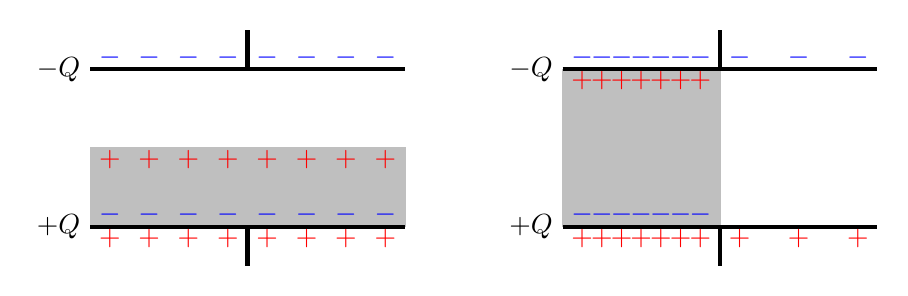
\begin{tikzpicture}
            \tikzstyle{wire} = [ultra thick]
            \tikzstyle{dielectric} = [fill=lightgray, color=lightgray]
            \tikzstyle{positive} = [color=red]
            \tikzstyle{negative} = [color=blue]
            \draw[dielectric] (0, 0) rectangle (4, 1);
            \draw[wire] (0, 0) -- (4, 0);
            \draw[wire] (0, 2) -- (4, 2);
            \draw[wire] (2, 0) -- (2, -0.5);
            \draw[wire] (2, 2) -- (2, 2.5);
            \node[left] at (0, 0) {\(+Q\)};
            \node[left] at (0, 2) {\(-Q\)};
            \foreach \x in {0.25, 0.75, ..., 3.75} {
                \node[positive] at (\x, 0.85) {\(+\)};
                \node[positive] at (\x, -0.15) {\(+\)};
                \node[negative] at (\x, 0.15) {\(-\)};
                \node[negative] at (\x, 2.15) {\(-\)};
            }
            
            \begin{scope}[xshift=6cm]
                \draw[dielectric] (0, 0) rectangle (2, 2);
                \draw[wire] (0, 0) -- (4, 0);
                \draw[wire] (0, 2) -- (4, 2);
                \draw[wire] (2, 0) -- (2, -0.5);
                \draw[wire] (2, 2) -- (2, 2.5);
                \node[left] at (0, 0) {\(+Q\)};
                \node[left] at (0, 2) {\(-Q\)};
                \foreach \x in {0.25, 0.5, ..., 1.75} {
                    \node[positive] at (\x, 1.85) {\(+\)};
                    \node[positive] at (\x, -0.15) {\(+\)};
                    \node[negative] at (\x, 0.15) {\(-\)};
                    \node[negative] at (\x, 2.15) {\(-\)};
                }
                \foreach \x in {2.25, 3, 3.75} {
                    \node[positive] at (\x, -0.15) {\(+\)};
                    \node[negative] at (\x, 2.15) {\(-\)};
                }
            \end{scope}
        \end{tikzpicture}
        \caption{The two interesting ways to half fill a capacitor with dielectric.}
        \label{fig:half filled capacitor}
    \end{figure}
    For the case of the capacitor half filled as shown on the left the addition of the dielectric does not break the planar symmetry of the situation and therefore \(\sigma_f\) is homogeneous.
    The high symmetry allows us to apply Gauss' law in media and from this we can get the displacement field and then from that we can get quantities of interest such as the electric field, polarisation field, bound charge density, potential, etc.
    For the case of the capacitor half filled as shown on the right the planar symmetry is broken and this means that Gauss' law is not as useful.
    By the symmetry of the situation we know that within the two regions, in the dielectric and outside the dielectric, the electric field is homogeneous.
    The free charge density, \(\sigma_f\), is inhomogeneous as the polarisation field distorts it.
    We therefore need to take a different approach to find the electric field we can construct equipotentials and then from the electric field we can find the displacement field and other interesting quantities.
    
    \section{The Magnetic Field in Media}
    \subsection{Types of Magnetisation}
    When an external magnetic field is applied to a material it will produce a magnetisation response.
    There are three mechanisms by which this can happen:
    \begin{itemize}
        \item Diamagnetism -- All materials have a diamagnetic response but it is only important in materials without an intrinsic magnetic moment as it is such a weak effect.
        What happens is the external magnetic field alters the angular momentum of the electrons which induces a field that opposes the external field.
        
        \item Paramagnetism -- This effect is important in materials in which each atom/molecule has an intrinsic magnetic moment and they are free to move.
        When an external field is applied these individual magnetic moments align with the field and create an induced field parallel to the applied field.
        
        \item Ferromagnetism -- This effect occurs in only a few materials.
        In these materials the intrinsic magnetic moments of individual species can align and stay aligned.
        However this is a local effect and the material will become a mosaic of `domains' where in each domain the magnetic moments of all species are aligned.
        When an external field is applied the domain boundaries will change in a way that favours domains where the magnetic moment is aligned with the external field.
        When the magnetic field is removed the domain boundaries do not return to where they where.
        This is the process by which a permanent magnet can be created.
    \end{itemize}
    
    \subsection{Magnetisation Field}
    The \define{magnetisation field}, \(\vv{M}\), is the net magnetisation dipole density in volume \(\dd{V}\):
    \[\dd{\vv{m}} = \vv{M}\dd{V}\]
    where \(\dd{\vv{m}}\) is the neg magnetic dipole moment due to the material in \(\dd{V}\).
    This is analogous to the definition of \(\vv{P}\) in section~\ref{sec:dielectric materials}.
    
    We can think of the magnetic dipole at a point as being the result of a small current loop.
    These then combine to give a macroscopic effect.
    \begin{figure}
        \centering
        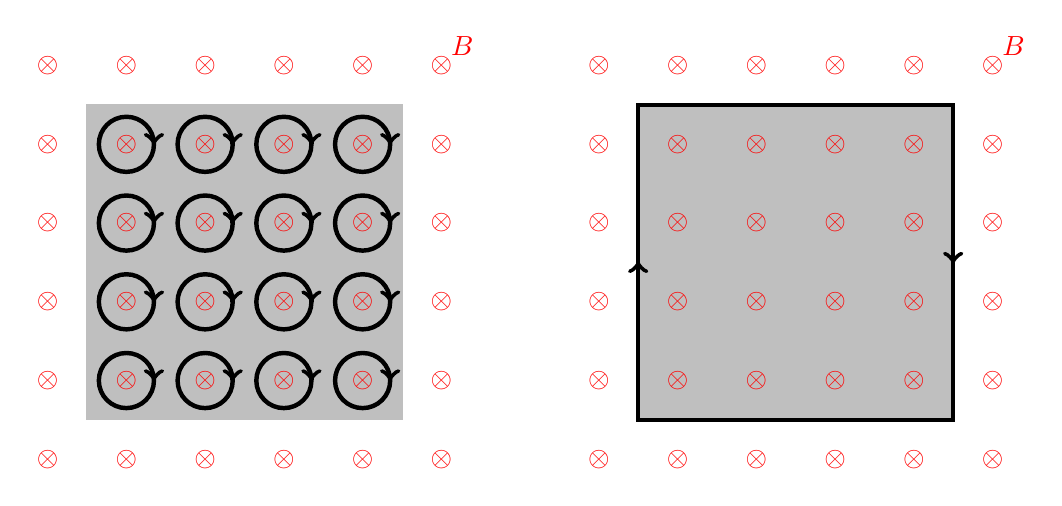
\begin{tikzpicture}
            \draw[fill=lightgray, color=lightgray] (0, 0)  rectangle (4, 4);
            \foreach \x in {0, 1, 2, 3} {
                \foreach \y in {0, 1, 2, 3} {
                    \draw[ultra thick] ($(\x, \y) + (0.5, 0.5)$) circle[radius=0.35cm];
                    \draw[ultra thick, ->] ($(\x, \y) + (0.85, 0.501)$) -- ($(\x, \y) + (0.85, 0.499)$);
                }
            }
            \foreach \x in {-0.5, 0.5, ..., 4.5} {
                \foreach \y in {-0.5, 0.5, ..., 4.5} {
                    \node[color=red] at (\x, \y) {\(\otimes\)};
                }
            }
            \node[color=red, above right] at (4.5, 4.5) {\(\vv{B}\)};
            
            \begin{scope}[xshift=1cm]
                \draw[fill=lightgray, ultra thick] (6, 0) rectangle (10, 4);
                \draw[ultra thick, ->] (10, 2.01) -- (10, 1.99);
                \draw[ultra thick, ->] (6, 1.99) -- (6, 2.01);
                \foreach \x in {5.5, 6.5, ..., 10.5} {
                    \foreach \y in {-0.5, 0.5, ..., 4.5} {
                        \node[color=red] at (\x, \y) {\(\otimes\)};
                    }
                }
                \node[color=red, above right] at (10.5, 4.5) {\(\vv{B}\)};
            \end{scope}
        \end{tikzpicture}
        \caption{Individual magnetic moments viewed as microscopic current loops vs. the net magnetic moment viewed as a macroscopic current loop.}
        \label{fig:magnetisation due to homogenous magnetic field}
    \end{figure}
    Figure~\ref{fig:magnetisation due to homogenous magnetic field} shows the net effect of many individual magnetic moments.
    In this case the magnetic field is homogenous and this results in there being no current in the material, \(\vv{J_M} = \vv{0}\).
    There is only a surface current, \(\vv{j_M}\).
    If the field were not homogenous then there would be an internal current.
    The magnetic moments for an inhomogeneous magnetic field are shown in figure~\ref{fig:magnetisation due to inhomogeneous magnetic field}
    \begin{figure}[ht]
        \centering
        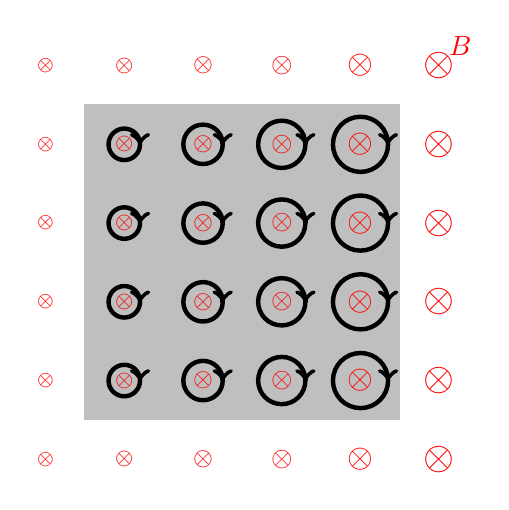
\begin{tikzpicture}
            \draw[color=lightgray, fill=lightgray] (0, 0) rectangle (4, 4);
            \foreach \y in {-0.5, 0.5, ..., 4.5} {
                \node[color=red] at (-0.5, \y) {\scriptsize \(\otimes\)};
                \node[color=red] at (0.5, \y) {\footnotesize \(\otimes\)};
                \node[color=red] at (1.5, \y) {\small \(\otimes\)};
                \node[color=red] at (2.5, \y) {\normalsize \(\otimes\)};
                \node[color=red] at (3.5, \y) {\large \(\otimes\)};
                \node[color=red] at (4.5, \y) {\Large \(\otimes\)};
            }
            \node[above right, color=red] at (4.5, 4.5) {\(\vv{B}\)};
            \foreach \y in {0.5, 1.5, ..., 3.5} {
                \draw[ultra thick] (0.5, \y) circle[radius=0.2cm];
                \draw[ultra thick, ->] ($(0.7, \y) + (0, 0.001)$) -- ($(0.7, \y) - (0, 0.001)$);
                \draw[ultra thick] (1.5, \y) circle[radius=0.25cm];
                \draw[ultra thick, ->] ($(1.75, \y) + (0, 0.001)$) -- ($(1.75, \y) - (0, 0.001)$);
                \draw[ultra thick] (2.5, \y) circle[radius=0.3cm];
                \draw[ultra thick, ->] ($(2.8, \y) + (0, 0.001)$) -- ($(2.8, \y) - (0, 0.001)$);
                \draw[ultra thick] (3.5, \y) circle[radius=0.35cm];
                \draw[ultra thick, ->] ($(3.85, \y) + (0, 0.001)$) -- ($(3.85, \y) - (0, 0.001)$);
            }
        \end{tikzpicture}
        \caption{Individual magnetic moments due to an inhomogeneous magnetic field.}
        \label{fig:magnetisation due to inhomogeneous magnetic field}
    \end{figure}
    In this case the eddy currents do not cancel and we have an internal current, \(\vv{J_M}\), as well as the surface current, \(\vv{j_M}\).
    
    We now want to quantify these effects.
    To do this we use the magnetic vector potential at \(\vv{r}\) due to an ideal magnetic dipole, \(\vv{m}\), at \(\vv{r'}\):
    \[\vv{A}(\vv{r}) = \frac{\mu_0}{4\pi} \frac{\vv{m}\times (\vv{r} - \vv{r'})}{\abs{\vv{r} - \vv{r'}}^3}.\]
    This generalises by superposition to
    \[\vv{A}(\vv{r}) = \frac{\mu_0}{4\pi} \int_V \frac{\vv{M}\times (\vv{r} - \vv{r'})}{\abs{\vv{r} - \vv{r'}}^3}\dd[3]{r'}.\]
    We then use the identity
    \[\frac{\vv{r} - \vv{r'}}{\abs{\vv{r} - \vv{r'}}^3} = \grad' \frac{1}{\abs{\vv{r} - \vv{r'}}}\]
    where \(\grad'\) is the gradient operator that acts only on \(\vv{r'}\).
    Hence
    \[\vv{A}(\vv{r}) = \frac{\mu_0}{4\pi} \int_V \vv{M}(\vv{r'}) \times \grad'\left[\frac{1}{\abs{\vv{r} - \vv{r'}}}\right] \dd[3]{r'}.\]
    We then use the product rule, \(\curl(f\vv{K}) = f\curl\vv{K} - \vv{K}\times\grad f\), to get
    \begin{align*}
        \vv{A}(\vv{r}) &= \frac{\mu_0}{4\pi} \int_V \frac{\grad'\times\vv{M}(\vv{r'})}{\abs{\vv{r} - \vv{r'}}} \dd[3]{r'} - \frac{\mu_0}{4\pi} \int_V \curl\left[\frac{\vv{M}(\vv{r'})}{\abs{\vv{r} - \vv{r'}}}\right] \dd[3]{r'}\\
        &= \frac{\mu_0}{4\pi} \int_V \frac{\grad'\times\vv{M}(\vv{r'})}{\abs{\vv{r} - \vv{r'}}} \dd[3]{r'} - \frac{\mu_0}{5\pi} \oint_S \left[\frac{\vv{M(\vv{r'})}}{\abs{\vv{r} - \vv{r'}}}\right]\times \dd{\vv{S'}}.
    \end{align*}
    Recall that
    \[\laplacian\vv{A} = \mu_0\vv{J} \implies \vv{A} = \frac{\mu_0}{4\pi} \int_V \frac{\vv{J}(\vv{r'})}{\abs{\vv{r} - \vv{r'}}}\dd[3]{r'}.\]
    This allows us to interpret the numerators of both integrands as currents.
    First
    \[\vv{J_M} = \curl\vv{M}\]
    is the bulk magnetisation current density, second
    \[\vv{j_M} = \vv{M}\times\vh{n}\]
    is the surface current density where \(\vh{n}\) is normal to the surface \(S'\) which bounds the volume \(V'\).
    
    \begin{example}
        A cylindrical bar magnet has uniform magnetisation, \(M\), along its axis.
        To what current distribution is this equivalent?
        
        \(\vv{M}\) is uniform so \(\curl\vv{M} = \vv{0}\) meaning \(\vv{J_M} = 0\).
        The surface current density is then
        \[\vv{j_M} = \vv{M}\times\vh{n} = M\ve{z}\times\ve{\rho} = M\ve{\varphi}.\]
        This has magnitude \(M\) and is `solenoidal', i.e. it resembles a solenoid with current flow around the circumference of a cylinder.
    \end{example}
    \begin{example}
        A long cylindrical bar magnet of uniform magnetisation is bent into a loop.
        To what current distribution is this equivalent?
        
        The curl in cylindrical coordinates is
        \[\curl\vv{M} = \left[\frac{1}{\rho}\pdv{M_z}{\varphi} - \pdv{M_\varphi}{z}\right]\ve{\rho} + \left[\pdv{M_\rho}{z} - \pdv{M_z}{\rho}\right]\ve{\varphi} + \frac{1}{\rho}\left[\pdv{\rho}(\rho M_\varphi) - \pdv{M_\rho}{\varphi}\right]\ve{z}.\]
        With this setup \(\vv{M}\) is circumferential so \(\vv{M} = M\ve{\varphi}\) so \(M_\rho = M_z = 0\) meaning that the curl reduces to
        \[\curl\vv{M} = \frac{1}{\rho}\pdv{\rho}(\rho M) = \frac{M}{\rho}\ve{z} = \vv{J_M}.\]
        The surface current has magnitude \(M\) and wraps around the cylinder still.
        The surface current is `toroidal', i.e. it resembles a toroidal solenoid with current flow over the surface.
        The bulk current density makes up for the fact that due to the geometry the net surface current is greater on the outside of the torus than the inside due to the greater surface area.
    \end{example}
    
    \subsection{Amp\`ere's Law in Media}
    The Amp\`ere--Maxwell law in a vacuum is
    \[\curl\vv{B} = \mu_0(\vv{J} + \varepsilon\partial_t\vv{E}).\]
    We divide \(\vv{J}\) into three parts: \(\vv{J_f}\) which is the current due to free charges, this is the normal current with which we have dealt so far, \(\vv{J_M} = \curl\vv{M}\) which is the magnetisation current as defined in the previous section, and \(\vv{J_P}\) which is the polarisation current which accounts for the movement of electric dipoles.
    To rationalise the introduction of \(\vv{J_P}\) we define a new charge density, \(\rho_P = -\div\vv{P}\), which follows the continuity equation
    \[\partial_t \rho_P + \div\vv{J_P} = 0.\]
    From this we have
    \[\vv{J_P} = \partial_t\vv{P}.\]
    We aim to write the Amp\`ere--Maxwell law in terms of \(\vv{J_f}\) only:
    \begin{align*}
        \curl\vv{B} &= \mu_0 (\vv{J_f} + \vv{J_M} + \vv{J_P} + \varepsilon_0\partial_t\vv{E})\\
        &= \mu_0(\vv{J_f} + \curl\vv{M} + \partial_t\vv{P} + \varepsilon_0\partial_t\vv{E})\\
        &= \mu_0(\vv{J_f} + \curl\vv{M} + \partial_t\vv{D})
    \end{align*}
    From this we have
    \[\curl\left[\frac{1}{\mu_0}\vv{B} - \vv{M}\right] = \vv{J_f} + \partial_t\vv{D}.\]
    We then define
    \[\vv{H} = \frac{1}{\mu_0}\vv{B} - \vv{M}\]
    so
    \[\curl\vv{H} = \vv{J_f} + \partial_t\vv{D}.\]
    This is the Amp\`ere--Maxwell law in media.
    In integral form it reads
    \[\oint_C \vv{H}\cdot\dd{\vv{l}} = \int_S (\vv{J_f} + \partial_t\vv{D})\cdot\dd{\vv{S}} = I_{f, \enc},\]
    where \(C\) is the contour bounding the surface \(S\).
    
    Confusingly \(\vv{H}\) is often referred to as the `magnetic field' and so is \(\vv{B}\).
    In some texts \(\vv{B}\) is the `magnetic flux density' and \(\vv{H}\) is the `magnetic field strength' but in other texts \(\vv{B}\) is the `magnetic field' and \(\vv{H}\) is the `auxiliary field'.
    For this reason it is best to specify `the magnetic \(\vv{B}\) field' or `the magnetic \(\vv{H}\) field'.
    
    Maxwell's second and third laws do not need modification in media as they contain no source terms, \(\rho\) or \(\vv{J}\).
    This means that we now have the four Maxwell equations in media:
    \begin{align*}
        \div\vv{D} &= \rho_f \tag{MI in media}\\
        \div\vv{B} &= 0 \tag{MII}\\
        \curl\vv{E} &= -\partial_t\vv{B} \tag{MIII}\\
        \curl\vv{H} &= \vv{J_f} + \partial_t\vv{D} \tag{MIV in media}
    \end{align*}
    
    We define the \define{magnetic susceptibility}, \(\chi_M\), to describe the relationship between \(\vv{M}\) and \(\vv{H}\):\footnote{some texts use \(\chi_B\vv{B} = \mu_0\vv{M}\) instead, these are related by \(\chi_B = \chi_M/(1 + \chi_M)\)}
    \[\vv{M} = \chi_M\vv{H}.\]
    In general \(\chi_M\) is a tensor however in \gls{lih} media it is a scalar.
    From this we also have
    \[\vv{B} = \mu_r\mu_0\vv{H} = \mu_0(1 + \chi_M)\vv{H} = \mu\vv{H}\]
    where \(\mu_r = 1 + \chi_M\) is the \define{relative permeability} and \(\mu = \mu_0\mu_r\) is the \define{absolute permeability}.
    In the absence of magnetisation \(\chi_M = 0\) and \(\mu_r = 1\).
    Unlike with dielectrics \(\chi_M\) can be positive or negative and consequently \(\mu_r\) is unbounded.
    For example a diamagnetic material will have \(\chi_M < 0\) whereas a paramagnetic material will have \(\chi_M > 0\) which corresponds to the fact that the fields induced in these two materials will be in opposite directions.
    
    \subsection{Media in Solenoids}
    A solenoid is filled with \gls{lih} medium with magnetic susceptibility \(\chi_M\).
    What is the effect compared to a solenoid containing a vacuum?
    
    The magnetisation field is given by \(\vv{M} = \chi_M\vv{H}\).
    The inductance of a solenoid is given by \(L = \Phi_B/I\).
    We first get \(\vv{H}\) from
    \[\curl\vv{H} = \vv{J_f} + \partial_t\vv{D} \implies \oint_C \vv{H}\cdot\dd{\vv{l}} = I_{f, \enc}.\]
    By symmetry we know that \(\vv{H}\) is axial and constant inside the solenoid and zero outside the solenoid.
    Thus if we define an Amp\'erian loop we only need integrate along the part inside the solenoid parallel to the axis.
    If this part has length \(l\) then
    \[\oint_C\vv{H}\cdot\dd{\vv{l}} = Hl = I_{f, \enc} = nlI \implies H_z = nI\]
    where \(n\) is the number of loops the solenoid has per unit length.
    From this we have
    \[\vv{B} = \mu_0\mu_r\vv{H} = \mu_0(1 + \chi_M)hI\ve{z}.\]
    This allows us to calculate the flux through the inductor treating the inductor as \(n\) loops of area \(A\) per unit length we have
    \[\Phi_B = ABnl = \mu_0(1 + \chi_M)n^2AlI\]
    where \(A\) is the cross sectional area of the solenoid.
    So the inductance is
    \[L = \frac{\Phi_B}{I} = \mu_0(1 + \chi_M)n^2Al = \mu_0(1 + \chi_M)n^2V_s\]
    where \(V_s = Al\) is the volume of the solenoid.
    
    \subsubsection{Partially Filled Solenoids}
    There are two interesting ways to half fill a solenoid.
    The first is with a cylindrical core which has a radius smaller than the solenoid.
    This preserves the cylindrical symmetry and therefore we can use Amp\`ere's law with two different cases, one that reaches all the way to the media and the other which stops in the vacuum.
    
    The second is with a cylindrical core that is of the same radius as the solenoid but doesn't extend for the solenoids entire length.
    This breaks the cylindrical symmetry.
    We can view this as two contributions, one from the filled section and one from the empty section.
    We cannot use Amp\`ere's law in this scenario to find the field.
    
    \section{Electromagnetism in Media}
    \subsection{Summary}
    Maxwell's equations for the macroscopic fields, \(\vv{D}\), \(\vv{B}\), \(\vv{E}\), and \(\vv{H}\), in media with free charge density, \(\rho_f\), and free current density, \(\vv{J_f}\), are
    \begin{align*}
        \div\vv{D} &= \rho_f, \tag{MI in media}\\ 
        \div\vv{B} &= 0, \tag{MII}\\
        \curl\vv{E} &= -\partial_t\vv{B},\tag{MIII}\\
        \curl\vv{H} &= \vv{J_f} + \partial_t\vv{D},\tag{MIV in media}
    \end{align*}
    Where the fields, \(\vv{D}\) and \(\vv{H}\), are defined as
    \[\vv{D} = \varepsilon_0\vv{E} + \vv{P},\qquad\text{and}\qquad \vv{B} = \mu_0(\vv{H} + \vv{M}).\]
    The free charges and currents satisfy the continuity equation
    \[\partial_t\rho_f + \div\vv{J_f} = 0.\]
    In \gls{lih} media the relations between the fields are
    \[\vv{P} = \chi_E\varepsilon_0\vv{E}, \qquad \vv{M} = \chi_M\vv{H}, \qquad \vv{D} = \varepsilon_0\varepsilon_r\vv{E} = \varepsilon\vv{E},\]
    \[\text{and}\qquad \vv{B} = \mu_0\mu_r\vv{H} = \mu\vv{H}.\]
    Where \(\varepsilon_r = 1 + \chi_E\) and \(\mu_r = 1 + \chi_M\).
    
    \subsection{Energy Density and the Poynting Vector}
    The power delivered by an \gls{em} field to a system of charge carriers is \(\vv{E}\cdot\vv{J_f}\) per unit volume.
    This means that the energy density, \(u\), obeys
    \[\dv{u}{t} = \vv{E}\cdot\vv{J_f}.\]
    We aim to express \(\vv{J_f}\) in field related quantities.
    First we use Maxwell's fourth law to write
    \[\vv{E}\cdot\vv{J_f} = \vv{E}\cdot\left[\curl\vv{H} - \partial_t\vv{D}\right] = \vv{E}\cdot(\curl\vv{H}) - \vv{E}\cdot\partial_t\vv{D}.\]
    We then use the product rule,
    \[\div(\vv{E}\times\vv{H}) = \vv{H}\cdot(\curl\vv{E}) - \vv{E}\cdot(\curl\vv{H}) \implies \vv{E}\cdot(\curl\vv{H}) - \vv{E}\cdot(\curl\vv{H}) - \div(\vv{E}\times\vv{H}),\]
    to get
    \[\vv{E}\cdot\vv{J} = \vv{H}\cdot(\curl\vv{E}) - \div(\vv{E}\times\vv{H}) - \vv{E}\cdot\partial_t\vv{D}.\]
    Using Maxwell's third law this becomes
    \[\vv{E}\cdot\vv{J_f} = -\vv{H}\cdot\partial_t\vv{B} - \div(\vv{E}\times\vv{H}) - \vv{E}\cdot\partial_t\vv{D}.\]
    Next we use that in \gls{lih} media
    \[\vv{E}\cdot\partial_t\vv{D} = \vv{E}\cdot\partial_t(\varepsilon\vv{E}) = \varepsilon\vv{E}\cdot\partial_t\vv{E} = \vv{D}\cdot\partial_t\vv{E}\]
    and
    \[\vv{H}\cdot\partial_t\vv{B} = \mu\vv{B}\cdot\partial_t\vv{B} = \vv{B}\cdot\partial_t(\mu\vv{B}) = \vv{B}\cdot\partial_t\vv{H}.\]
    This gives us
    \[\vv{E}\cdot\vv{J_f} = -\vv{B}\cdot\partial_t\vv{H} - \vv{D}\cdot\partial_t\vv{E} - \div(\vv{E}\times\vv{H}).\]
    Recognising the standard product rule
    \[\partial_t(\vv{E} \cdot \vv{D}) = \vv{D}\cdot\partial_t\vv{E} + \vv{E}\cdot\partial_t\vv{D} = 2\vv{D}\cdot\partial_t\vv{E}\]
    and similarly for the magnetic fields this becomes
    \[\vv{E}\cdot\vv{J_f} = \frac{1}{2}\partial_t(\vv{E}\cdot\vv{D} + \vv{B}\cdot\vv{H}).\]
    We then integrate over a volume, \(V\), to get the energy from the energy density.
    Using the divergence theorem on the second term we get
    \[\dv{U}{t} = -\frac{1}{2}\dv{t}\int_V (\vv{E}\cdot\vv{D} + \vv{B}\cdot\vv{H})\dd{V} - \oint_A(\vv{E}\times\vv{H})\cdot\dd{\vv{A}}.\]
    We now identify the electric and magnetic energy densities as
    \[u_E = \frac{1}{2}\vv{E}\cdot\vv{D}, \qquad\text{and}\qquad u_M = \frac{1}{2}\vv{B}\cdot\vv{H}\]
    respectively.
    From the second term we identify the macroscopic Poynting vector as
    \[\vv{S} = \vv{E}\times\vv{H}\]
    so the power delivered to the charges can be written as
    \[\dv{U}{t} = -\dv{t}[U_E + U_M] - \oint_A\vv{S}\cdot\dd{\vv{A}}.\]
    
    \subsection{Boundary Conditions}
    \subsubsection{Qualitatively}
    Now that we have characterised fields in and out of media we want to know how the fields behave at the boundary between media.
    To do this we use the work we have done already with half filled capacitors/inductors and we make the unjustified assumption that the same analysis holds outside of a capacitor/inductor.
    Figure~\ref{fig:fields at boundaries} shows qualitatively what happens at a boundary for the four fields, this figure assumes that \(\chi_M > 0\).
    The two cases we consider for each field are what happens to the tangential component and the normal component at the boundary.
    \begin{figure}[ht]
        \centering
        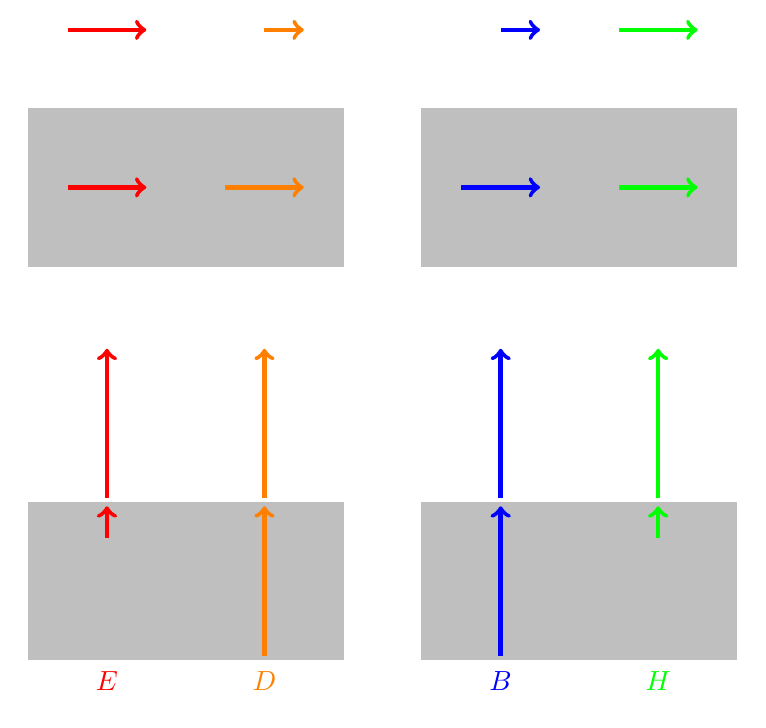
\begin{tikzpicture}
            \tikzstyle{media} = [fill=lightgray, color=lightgray]
            \tikzstyle{field} = [ultra thick, ->]
            \tikzstyle{E} = [field, color=red]
            \tikzstyle{B} = [field, color=blue]
            \tikzstyle{D} = [field, color=orange]
            \tikzstyle{H} = [field, color=green]
            \draw[media] (0, 0) rectangle (4, 2);
            \draw[media] (5, 0) rectangle (9, 2);
            \draw[media] (0, 5) rectangle (4, 7);
            \draw[media] (5, 5) rectangle (9, 7);
            \draw[E] (1, 1.55) -- (1, 1.95);
            \draw[E] (1, 2.05) -- (1, 3.95);
            \draw[D] (3, 0.05) -- (3, 1.95);
            \draw[D] (3, 2.05) -- (3, 3.95);
            \draw[E] (0.5, 6) -- (1.5, 6);
            \draw[E] (0.5, 8) -- (1.5, 8);
            \draw[D] (2.5, 6) -- (3.5, 6);
            \draw[D] (3, 8) -- (3.5, 8);
            \draw[B] (6, 0.05) -- (6, 1.95);
            \draw[B] (6, 2.05) -- (6, 3.95);
            \draw[H] (8, 1.55) -- (8, 1.95);
            \draw[H] (8, 2.05) -- (8, 3.95);
            \draw[B] (5.5, 6) -- (6.5, 6);
            \draw[B] (6, 8) -- (6.5, 8);
            \draw[H] (7.5, 6) -- (8.5, 6);
            \draw[H] (7.5, 8) -- (8.5, 8);
            
            \node[below, E] at (1, 0) {\(\vv{E}\)};
            \node[below, D] at (3, 0) {\(\vv{D}\)};
            \node[below, B] at (6, 0) {\(\vv{B}\)};
            \node[below, H] at (8, 0) {\(\vv{H}\)};
        \end{tikzpicture}
        \caption{The qualitative behaviour of fields at a boundary between media. The normal and tangential components of the four fields are shown both in the media and outside.}
        \label{fig:fields at boundaries}
    \end{figure}
    \subsubsection{Quantitatively}
    We can be much more rigorous if we use Maxwell's laws.
    We assume we have a plane and above and below the plane are two different media, media 1 below and media 2 above.
    We use a Gaussian surface that is a cylindrical pill box of height \(h\) with the flat faces parallel to the plane, and a rectangular Amp\'erian loop of height \(h\) with two sides running parallel to the plane.
    We also define two vectors, \(\vh{n}\), and \(\vh{t}\), which are normal and tangential to the plane respectively.
    
    The first condition we consider is Maxwell's first law,
    \[\div\vv{D} = \rho_f.\]
    From this and the divergence theorem we have
    \[\oint_S\vv{D}\cdot\dd{\vv{S}} = Q_{f, \enc}.\]
    pill box has a surface normal, on the flat faces, of \(\dd{\vv{S}} = \vh{n}\dd{S}\).
    Allowing \(h\to 0\) we can ignore the contribution to the integral from the sides of the pill box and we get
    \[\int\vv{D}\cdot\dd{\vv{S}} = \int(\vv{D_2} - \vv{D_1})\cdot\vh{n}\dd{S} = \int \sigma_f \dd{S}\]
    where the last equality arises from the definition of a surface charge density.
    Note that \(\vv{D_1}\) is the \(\vv{D}\) field below the plane and \(\vv{D_2}\) is the \(\vv{D}\) field above the plane.
    Since both integrals are over the same area we can conclude that
    \[(\vv{D_2} - \vv{D_1})\cdot\vh{n} = \sigma_f.\]
    Taking the scalar product with \(\vh{n}\) picks out the scalar component of \(\vv{D_2} - \vv{D_1}\) and so \(\vv{D_{\mathrm{normal}}}\) is continuous \emph{if and only if} \(\sigma_f = 0\).
    
    The second condition we consider is Maxwell's second law,
    \[\div\vv{B} = 0 \implies \oint_S \vv{B}\cdot\dd{\vv{S}} = 0.\]
    Using the same Gaussian surface and again allowing \(h\to 0\) we have
    \[\int\vv{B}\cdot\dd{\vv{S}} = \int (\vv{B_2} - \vv{B_1})\cdot\vh{n}\dd{S} = 0.\]
    This holds for any similarly defined surface so
    \[(\vv{B_2} - \vv{B_1})\cdot\vh{n} = 0\]
    meaning that \(\vv{B_{\mathrm{normal}}}\) is \emph{always} continuous.
    
    The third condition we consider is Maxwell's third law,
    \[\curl\vv{E} = -\partial_t\vv{B} \implies \oint_C\vv{E}\cdot\dd{\vv{l}} = -\partial_t\Phi_B.\]
    We use an Amp\'erian loop of length \(\ell\) and height \(h\).
    Allowing \(h\to -\) we also have \(\Phi_B\to 0\) as long as \(B\) is finite.
    Therefore
    \[\int \vv{E}\cdot\dd{\vv{l}} = \int(\vv{E_2} - \vv{E_1})\cdot\vh{t} \dd{l} = 0\]
    where \(\vh{t}\) is tangential to the surface meaning that \(\vh{t}\cdot\vh{n} = 0\).
    Since this holds no matter where we put the Amp\'erian loop, or define \(\vh{t}\) we have
    \[(\vv{E_2} - \vv{E_1})\cdot\vh{t} = 0\]
    meaning that \(\vv{E_{\mathrm{tangential}}}\) is \emph{always} continuous.
    
    The final condition that we consider is Maxwell's fourth law
    \[\curl\vv{H} = \vv{J_f} + \partial_t\vv{D}\]
    in integral form this becomes
    \[\oint_{C}\vv{H}\cdot\dd{\vv{l}} = \vv{j_f} \cdot \vh{s}\ell + (\partial_t\vv{D})\cdot\vh{s}\ell h\]
    where \(\vv{j_f}\) is the free surface current per unit area and \(\vh{s} = \vh{t}\times\vh{n}\) is the surface unit vector perpendicular to the Amp\'erian loop.
    Now allowing \(h\to 0\) we have
    \[\int\vv{H}\cdot\dd{\vv{l}} = \vv{H_1} - \vv{H_2})\cdot\vh{t}\ell = \vh{j_f}\cdot\vh{s}\ell.\]
    Since \(\vh{n}\) is normal to the plane \(\vh{s}\) is tangential to the plane so \(\vv{H_\mathrm{tangential}}\) is continuous \emph{if and only if} \(\vv{j_f} = \vv{0}\).
    This general form can be written in other ways, including
    \begin{align*}
        (\vv{H_1} - \vv{H_2})\cdot\vh{t} &= \vv{j_f}\cdot\vh{s},\\
        (\vv{H_{2, \mathrm{tangential}}} - \vv{H_{1, \mathrm{tangential}}}) &= \vv{j_f}\times\vh{n},\\
        (\vv{H_2} - \vv{H_1})\times\vh{n} &= -\vv{j_f}.
    \end{align*}

    In summary at a boundary between media
    \begin{itemize}
        \item \(\vv{D_{\mathrm{normal}}}\) is continuous if and only if \(\sigma_f = 0\).
        \item \(\vv{B_{\mathrm{normal}}}\) is continuous always.
        \item \(\vv{E_{\mathrm{tangential}}}\) is continuous always.
        \item \(\vv{H_{\mathrm{tangential}}}\) is continuous if and only if \(\vv{j_f} = \vv{0}\).
    \end{itemize}

    \section{Continuity Conditions and Waves in Media}
    \subsection{Applications of Continuity Conditions}
    \subsubsection{Inclined Dielectric}
    Consider the setup in figure~\ref{fig:refraction}.
    \begin{figure}[ht]
        \centering
        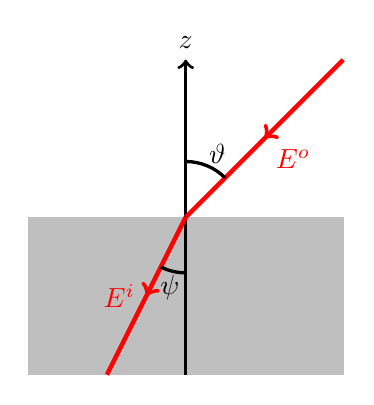
\begin{tikzpicture}
            \tikzstyle{mid arrow} = [postaction={decorate, decoration={markings, mark=at position .5 with {\arrow{>}}}}]
            \tikzstyle{E base} = [ultra thick, color=red]
            \tikzstyle{E} = [E base, mid arrow]
            \tikzstyle{angle} = [very thick]
            \tikzstyle{media} = [color=lightgray, fill=lightgray]
            \tikzstyle{axis} = [very thick, ->]
            \draw[media] (-2, -2) rectangle (2, 0);
            \draw[axis] (0, -2) -- (0, 2) node[above] {\(z\)};
            \draw[E] (2, 2) -- (0, 0);
            \draw[E] (0, 0) -- (-1, -2);
            \draw[angle] (0.5, 0.5) arc[start angle=45, end angle=90, radius=0.707cm];
            \draw[angle] (0, -0.707) arc[start angle=-90, end angle=-116.6, radius=0.707cm];
            \node[below right, E base] at (1, 1) {\(\vv{E^o}\)};
            \node[left, E base] at (-0.5, -1) {\(\vv{E^i}\)};
            \node at (0.4, 0.8) {\(\vartheta\)};
            \node at (-0.2, -0.9) {\(\psi\)};
        \end{tikzpicture}
        \caption{An inclined dielectric with an incident electric field.}
        \label{fig:refraction}
    \end{figure}
    It shows a uniform electric field, \(\vv{E^o}\), incident on a dielectric at an angle \(\vartheta\).
    The field is then refracted and the field in the dielectric is at an angle \(\psi\).
    We want to know what the field, \(\vv{E^i}\), inside the dielectric is.
    
    Outside the dielectric we define the displacement field as
    \[\vv{D^o} = \varepsilon_0\vv{E^o}.\]
    Inside the dielectric the displacement field is
    \[\vv{D^i} = \varepsilon_0\varepsilon_r\vv{E^i}.\]
    We apply the boundary condition that the normal component of the displacement field, \(D_n\), is continuous at the boundary, since there is no surface charge.
    This means that \(D^o_z = D^i_z\).
    The second boundary condition is that the tangential components of the electric field, \(E_t\), are continuous at the boundary.
    This means that \(E^o_x = E^i_x\) and \(E^o_y = E^i_y\).
    We choose a coordinate system such that \(E^o_y = E^i_y = 0\) meaning that we can work in the two-dimensional \((x, z)\)-plane.
    In this plane the full fields are
    \[\vv{E^o} = (E^o\sin\vartheta, E^o\cos\vartheta), \qquad\text{and}\qquad \vv{E^i} = (E^i\sin\psi, E^i\cos\psi).\]
    Applying the first continuity condition we have
    \[D^o_z = D_i^z \implies \varepsilon_0E^o\cos\vartheta = \varepsilon_0\varepsilon_rE^i\cos\psi \implies E^i = \frac{1}{\varepsilon_r}E^o\frac{\cos\vartheta}{\cos\psi}.\]
    Applying the second continuity condition we have
    \[E^o_x = E^i_x \implies E^o\sin\vartheta = E^i\sin\psi \implies E^i = E^o\frac{\sin\vartheta}{\sin\psi}.\]
    Combining these we have
    \[\frac{1}{\varepsilon_r}\frac{\cos\vartheta}{\cos\psi} = \frac{\sin\vartheta}{\sin\psi} \implies \frac{\sin\psi}{\cos\psi} = \tan\psi = \varepsilon_r\frac{\sin\vartheta}{\cos\vartheta} = \varepsilon_r\tan\vartheta \implies \psi = \arctan(\varepsilon_r\tan\vartheta).\]
    It is worth checking two basic case here.
    First we consider the case when \(\vartheta = 0\).
    In this case \(\psi = \arctan(\varepsilon_r\tan 0) = \arctan 0 = 0\) and so there is no refraction which is what we would expect.
    Going a step further back in the calculation if \(\psi = \vartheta = 0\) then we recover that \(D^o_z = D^i_z\).
    The second case we consider is \(\vartheta = \pi/2\).
    In this case \(\psi = \arctan(\varepsilon_r\tan(\pi/2)) = \arctan(\infty) = \pi/2\) and so there is no refraction as the field travels along the boundary.
    Going a step further back in the calculation if \(\psi = \vartheta = \pi/2 \) then we recover \(E^o = E^i\).
    
    \subsubsection{Spherical Cavity in a Dielectric}
    Suppose we have a large block of \gls{lih} dielectric which contains a spherical cavity.
    The electric field far from the cavity is uniform and has magnitude \(E_0\).
    What are \(\vv{E}\) and \(\vv{D}\) in the cavity?
    
    We will use spherical coordinates with their origin at the centre of the cavity and aligned so that the \(z\)-axis is parallel to the field at large \(r\).
    See figure~\ref{fig:spherical cavity} for a diagram.
    \begin{figure}[ht]
        \centering
        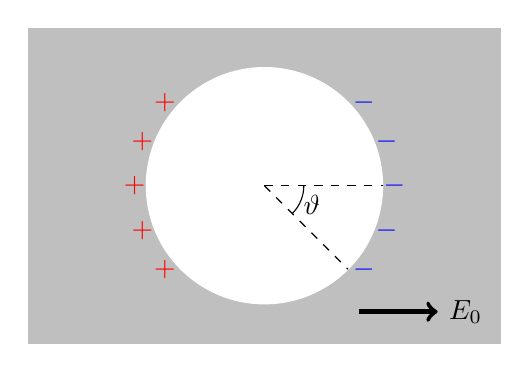
\begin{tikzpicture}
            \tikzstyle{media} = [color=lightgray, fill=lightgray]
            \tikzstyle{E} = [->, ultra thick]
            \draw[media] (-3, -2) rectangle (3, 2);
            \draw[fill=white, color=white] (0, 0) circle[radius=1.5cm];
            \draw[dashed] (0, 0) -- (1.5, 0);
            \draw[dashed] (0, 0) -- (1.06, -1.06);
            \draw (0.5, 0) arc[start angle=0, end angle=-45, radius=0.5cm];
            \node at (-22.5:0.65) {\(\vartheta\)};
            \foreach \x in {0, -20, 20, 40, -40} {
                \node[color=red] at ($({-1*cos(\x)*1.65}, {sin(\x)*1.65})$) {\(+\)};
                \node[color=blue] at ($({cos(\x)*1.65}, {sin(\x)*1.65})$) {\(-\)};
            }
            \draw[E] (1.2, -1.6) -- (2.2, -1.6) node[right] {\(\vv{E_0}\)};
        \end{tikzpicture}
        \caption{A spherical cavity in a dielectric}
        \label{fig:spherical cavity}
    \end{figure}
    At the surface of the cavity a charge distribution, \(\sigma_P = \vv{P}\cdot\vh{n}\) forms.
    Note that \(\vh{n}\) is the outward normal of the dielectric, meaning it points \emph{towards} the origin.
    Since this is an \gls{lih} media \(\vv{P}\) is parallel to \(\vv{E}\) and so the field inside is enhanced by the charge distribution which is a function of the angle, \(\vartheta\), since \(r = 1.5\) on the surface of the cavity and the symmetry under changing \(\varphi\) means that \(\sigma_P\) cannot depend on \(\varphi\).
    
    The charge distribution, \(\sigma_P(\vartheta)\), forms an effective dipole.
    Outside of the cavity the field lines are locally distorted by this charge distribution.
    We want to determine \(V\), the electrostatic potential, and from this we can calculate \(\vv{E}\).
    Within the cavity we assume a uniform \(\vv{E}\) field in the \(z\) direction.
    This corresponds to a potential
    \[V(r) = -E_{\text{in}}z = -E_{\text{in}}r\cos\vartheta\]
    for \(r < a\) where \(a\) is the radius of the cavity.
    Outside of the cavity we use a superposition of a uniform \(\vv{E_0}\) field plus a dipole field so
    \[V(r) = -E_0r\cos\vartheta + \frac{A\cos\vartheta}{r^2}.\]
    Here \(A\) is a constant to be found which gives the relative strength of the dipole field.
    
    Thanks to the uniqueness theorem for Poisson's equation we need only show that this potential fulfils the boundary conditions and Poisson's equation and then we know that the electric field derived from this potential is unique.
    Since the charges are only on the boundary away from the boundary we only need the potential to satisfy Laplace's equation, \(\laplacian V = 0\).
    We then only need to check that the boundary conditions are satisfied.
    In spherical coordinates
    \[\grad V = \ve{r}\pdv{V}{r} + \ve{\vartheta}\frac{1}{r}\pdv{V}{\vartheta} + \ve{\varphi}\frac{1}{r\sin\vartheta}\pdv{V}{\vartheta} = -\vv{E}.\]
    The first boundary condition we check is that \(E_t\) is continuous.
    This requires \(E_\vartheta\) to be continuous at \(r = a\).
    So
    \[-E_0a\sin\vartheta + \frac{A\sin\vartheta}{a^2} = -E_{\text{in}}a\sin\vartheta.\]
    The second boundary condition is that \(D_n\) is continuous (note the surface density is due to polarisation, there is no free charge distribution).
    This requires \(D_r = \varepsilon_rE_r = -\varepsilon_r\partial_rV\) to be continuous.
    So
    \[\varepsilon_rE_o\cos\vartheta + \frac{2A\varepsilon_r\cos\vartheta}{a^3} = E_{\text{in}}\cos\vartheta.\]
    Combining these we have
    \[E_{\text{in}} = \varepsilon_r\left(E_0 + \frac{2A}{a^3}\right) = E_0 - \frac{A}{a^3}.\]
    Thus
    \[E_{\text{in}} = E_0\frac{3\varepsilon_r}{1 + 2\varepsilon_r}.\]
    Combining this with the requirement that \(\vv{E_{\mathrm{in}}} = E_{\mathrm{in}}\ve{z}\) and \(\vv{D_{\mathrm{in}}} = \varepsilon_0\vv{E_{\mathrm{in}}}\) (since inside the cavity \(\varepsilon_r = 1\)), we have the full field.
    Notice that \(E_{\text{in}} > E_0\) so the field in the cavity is stronger than the field outside.
    
    \subsection{Waves in Media}
    \subsubsection{Non-conduction Media}
    In a non-conducting media \(\rho_f = 0\) and \(\vv{J_f} = 0\).
    Thus
    \[\vv{D} = \varepsilon\vv{E}, \qquad\text{and}\qquad \vv{B} = \mu\vv{H}.\]
    We can derive macroscopic wave equations as before:
    \[\laplacian\vv{E} = \varepsilon\mu \pdv[2]{\vv{E}}{t}, \qquad\text{and}\qquad \laplacian\vv{B} = \varepsilon\mu\pdv[2]{\vv{B}}{t}.\]
    Clearly these have the normal plane wave solutions
    \[\vv{E} = \vv{E_0}e^{i(\vv{k}\cdot\vv{r} - \omega t)}, \qquad\text{and}\qquad \vv{B} = \vv{B_0}e^{i(\vv{k}\cdot\vv{r} - \omega t)}.\]
    Where \(k^2 = \mu\varepsilon\omega^2\).
    We interpret this as the wave phase velocity being
    \[v = \frac{\omega}{k} = \frac{1}{\sqrt{\mu\varepsilon}}.\]
    Recall that \(c = (\mu_0\varepsilon_0)^{-1/2}\) so
    \[v^2 = \frac{1}{\mu_r\varepsilon_r}c^2 = \frac{1}{n^2}c^2\]
    where we have defined \(n = \mu_r\varepsilon_r\) which is called the \define{refractive index} and is a property of the medium.
    As we did with waves in a vacuum it can be shown that
    \[i\vv{k}\cdot\vv{E_0} = 0, \qquad\text{and}\qquad i\vv{k}\cdot\vv{B_0} = 0.\]
    This means that \(\vv{E}\) and \(\vv{B}\) are perpendicular to the direction of propagation, \(\vv{k}\), and therefore the wave is transverse.
    We see that for \gls{lih} media all of the extra complications that come with having media are neatly hidden away in \(\varepsilon\) and \(\mu\) and have the net effect of changing the velocity of the wave.
    
    \subsubsection{Waves in Conductors}
    In conductors in general \(\rho_f \ne 0\) and \(\vv{J_f} \ne \vv{0}\).
    We will start with Ohm's law, \(\vv{J} = \sigma\vv{E}\) and assume linear media so
    \[\vv{D} = \varepsilon\vv{E}, \qquad\text{and}\qquad \vv{B} = \mu\vv{H}.\]
    Combining these with Maxwell's fourth equation gives us
    \begin{equation}\label{eqn:curl B}
        \curl\vv{H} = \vv{J_f} + \partial_t\vv{D} \implies \curl\vv{B} = \mu\sigma\vv{E} + \mu\varepsilon\partial_t\vv{E}.
    \end{equation}
    Taking the curl of Maxwell's third equation we have
    \[\curl(\curl\vv{E}) = \grad(\div\vv{E}) - \laplacian\vv{E} = -\curl(\partial_t\vv{B}) = -\partial_t(\curl\vv{B}).\]
    Substituting for \(\curl\vv{B}\) from equation~\ref{eqn:curl B} we have
    \[\partial_t\left(\mu\sigma\vv{E} + \mu\varepsilon\partial_t\vv{E}\right) = \laplacian\vv{E} - \grad\left(\frac{\rho}{\varepsilon}\right) = \laplacian\vv{E}\]
    where in the last equality we assume a uniform charge density meaning that \(\grad\rho = 0\).
    Rearranging this we have
    \[\laplacian\vv{E} = \mu\varepsilon\pdv[2]{\vv{E}}{t} + \mu\sigma\pdv{\vv{E}}{t}.\]
    Notice that this is the wave equation with an additional term on the right.
    The origin of this additional term is the free current.
    
    Taking the curl of Maxwell's fourth equation gives us
    \[\curl(\curl\vv{B}) = \grad(\div\vv{B}) - \laplacian\vv{B} = \mu\sigma\curl\vv{E} + \mu\varepsilon\partial_t(\curl\vv{E}).\]
    Substituting for Maxwell's second and third laws we have
    \[\laplacian\vv{B} =  \mu\varepsilon\partial_t\pdv[2]{\vv{B}}{t} + \mu\sigma\pdv{\vv{B}}{t}.\]
    
    \section{Waves In Conductors}
    We saw in the last section that we could derive wave equations in conductors which, if we assume linear media, have the form
    \[\laplacian\vv{E} = \mu\varepsilon\pdv[2]{\vv{E}}{t} + \mu\sigma\pdv{\vv{E}}{t}.\]
    We make the ansatz that this has the plane wave solution
    \[\vv{E} = \tilde{\vv{E}}e^{i(\tilde{k}z - \omega t)}\]
    where we assume the wave is travelling in the \(z\) direction.
    If we substitute this into the wave equation we get
    \[\tilde{k}^2 = \mu\varepsilon\omega^2 + i\mu\sigma\omega.\]
    This is the \define{dispersion relation}.
    To solve this we clearly need to consider some complex numbers.
    Let \(\tilde{k} = k + i\kappa\) for some \(k, \kappa\in\reals\).
    Then if we equate real and imaginary parts in the dispersion relation we have
    \[k^2 - \kappa^2 = \mu\varepsilon\omega^2, \qquad\text{and}\qquad 2k\kappa = \mu\sigma\omega.\]
    The second of these has the solution \(\kappa = \mu\sigma\omega/2k\) which allows us to eliminate \(\kappa\) from the first giving
    \[k^4 - \left(\frac{\mu\sigma\omega}{2}\right)^2 = \mu\varepsilon\omega^2k^2.\]
    This is a quadratic in \(k^2\) and has the solution
    \[k^2 = \frac{1}{2}\mu\varepsilon\omega^2 = \frac{1}{2}\left[(\mu\varepsilon\omega^2)^2 + (\mu\sigma\omega)^2\right]^{1/2} = \frac{\mu\varepsilon\omega^2}{2}\left[\left(1 + \left[\frac{\sigma}{\varepsilon\omega}\right]^2\right)^{1/2} + 1\right],\]
    where we choose the positive square root so that \(k^2\) is positive, since \(k\in\reals\).
    We can then use this to obtain
    \[\kappa^2 = \frac{\mu\varepsilon\omega^2}{2}\left[\left(1 + \left[\frac{\sigma}{\varepsilon\omega}\right]^2\right)^{1/2} - 1\right].\]
    Hence
    \[\vv{E} = \tilde{\vv{E_0}}e^{-\kappa z}e^{i(kz - \omega t)}.\]
    This describes exponential decay of the wave along \(z\), which is the propagation direction.
    The wave is attenuated over a characteristic distance, called the \define{skin depth}, which is given by
    \[\delta = \frac{1}{\kappa}.\]
    This gives the depth at which the amplitude of the wave is \(e^{-1}\) times the amplitude at which the wave enters the conductor.
    
    A good check to do here is consider the case when \(\sigma = 0\), this corresponds to a vacuum.
    In this case \(k^2 = \varepsilon\mu\omega^2\) and \(\kappa^2 = 0\) so we revert to the vacuum solution.
    
    \subsection{Good and Poor Conductors}
    The ratio \(\sigma/\varepsilon\omega\) is important in this result.
    Both \(1/\omega\) and \(\varepsilon/\sigma\) have units of time so this quantity is a ratio of two timescales.
    The question now is what do these timescales represent?
    
    Consider the continuity equation for free charges,
    \[\partial_t\rho_f + \div\vv{J_f} = 0.\]
    Using Ohm's law, \(\vv{J_f} = \sigma\vv{E}\) we have 
    \[\div\vv{J_f} = \sigma\div\vv{E} = \frac{\sigma}{\varepsilon}\div\vv{D} = \frac{\sigma}{\varepsilon}\rho_f\]
    so the continuity equation becomes
    \[\partial_t\rho_f = -\frac{\sigma}{\varepsilon}\rho_f.\]
    This has as a solution
    \[\rho_f(t) = \rho_f(0)e^{-\sigma t/\varepsilon}.\]
    So \(\varepsilon/\sigma\) is the characteristic timescale for how fast charge decays in a conductor.
    This is known as the \define{relaxation time}, \(\tau\).
    This quantity tells us how fast charges migrate to the surface and how fast the electric field disappears in a conductor.
    In an ideal conductor \(\sigma \to \infty\) and \(\tau \to 0\) which corresponds to our assumption for an ideal conductor that charge is always concentrated on the surface and \(\vv{E} = \vv{0}\) inside an ideal conductor.
    
    The interpretation of \(1/\omega\) is, as one would expect, the period of the wave, \(T = 2\pi/\omega\).
    Thus \(\sigma/\varepsilon\omega = T/2\pi\tau\).
    We use this ratio to characterise conductors as ``good" and ``bad".
    For a ``good" conductor \(\sigma/\varepsilon\omega \gg 1\).
    For a ``bad" conductor \(\sigma/\varepsilon\omega \ll 1\).
    Notice that how ``good" a conductor is depends on the frequencies that we care about transmitting.
    For example it is possible that a conductor can be a good conductor of radio waves, which have a relatively small value of \(\omega\), and a bad conductor of ultraviolet, which has a large value of \(\omega\).
   
    
    It can be shown that for a good conductor
    \[\delta \approx \sqrt{\frac{2}{\mu\omega\sigma}},\]
    and for a bad conductor
    \[\delta \approx \sqrt{\frac{4\varepsilon}{\mu\sigma^2}}.\]
    Typical metals are good conductors up to about \SI{1}{\mega\hertz} with \(\delta \approx \SI{1}{\centi\meter}\) at \SI{50}{\hertz} (mains power frequency) and \(\delta \approx \SI{10}{\micro\meter}\) at \SI{50}{\mega\hertz}.
    
    Some consequences of the skin depth are
    \begin{itemize}
        \item Cables greater than about \SI{1}{\centi\meter} in width are wasted as the current is mostly in the skin layer around the outside and there is a `dead zone' in the centre.
        Cables that initially seem thicker than \SI{1}{\centi\meter} are often actually multiple narrower cables bound together.
        \item Submarines cannot use radio as at the typical depth of a submarine radio waves simply cannot penetrate the water.
        \item Mobile phones don't work inside metal boxes as they use radio waves which have frequencies in the gigahertz range and therefore don't penetrate very far through metal.
        \item Microwave oven doors have a metal mesh with holes much smaller than the wavelength of the microwaves.
        This allows visible light through but not microwaves.
    \end{itemize}

    \subsection{Phase Relations of Fields}
    As with waves in a vacuum or insulator Maxwell's first and second laws imply that
    \[i\tilde{\vv{k}}\cdot\tilde{\vv{E_0}} = 0, \qquad\text{and}\qquad i\tilde{\vv{k}}\cdot\tilde{\vv{B_0}} = 0\]
    so the waves are transverse.
    In the case that \(\tilde{\vv{k}} = \tilde{k}\ve{z}\) and \(\tilde{\ve{E_0}} = \tilde{E_0}\ve{x}\) if we substitute into Maxwell's third equation we get
    \[i\tilde{\vv{k}}\times\tilde{\vv{E_0}} = i\omega\tilde{\vv{B_0}}\]
    hence
    \begin{equation}\label{eqn:B0 = kE0/omega ey}
        \tilde{\vv{B_0}} = \frac{\tilde{k}\tilde{E_0}}{\omega}\ve{y}.
    \end{equation}
    In general \(\tilde{k}\) is complex and therefore so are \(\tilde{E_0}\) and \(\tilde{B_0}\).
    We write
    \[\tilde{k} = Re^{i\varphi}, \qquad\text{where}\qquad R = \sqrt{k^2 + \kappa^2}, \qquad\text{and}\qquad \varphi = \arctan\left(\frac{\kappa}{k}\right).\]
    Then
    \[\tilde{E_0} = E_0e^{i\delta_E}, \qquad\text{and}\qquad \tilde{B_0} = B_0e^{i\delta_B}.\]
    Substituting these into equation~\ref{eqn:B0 = kE0/omega ey} we get
    \[B_0e^{i\delta_B} = \frac{Re^{i\varphi}}{\omega}E_0e^{i\delta_E} \implies \delta_B - \delta_E = \varphi.\]
    What this means is that the magnetic field has a phase of \(\varphi\) behind the electric field since when we take the real part to get the physical fields we get
    \begin{align*}
        \vv{E} &= E_0e^{-\kappa z}\cos(kz - \omega t + \delta_E)\ve{x},\\
        \vv{B} &= B_0e^{-\kappa z}\cos(kz - \omega t + \delta_E + \varphi)\ve{y}.
    \end{align*}
    In terms of physical constants we have
    \[R = \sqrt{k^2 + \kappa^2} = \omega\sqrt{\mu\varepsilon}\left[1 + \left(\frac{\sigma}{\varepsilon\omega}\right)^2\right]^{1/4},\]
    and
    \[\varphi = \arctan\left(\frac{\kappa}{k}\right)  = \arctan\left(\left[\frac{\sqrt{1 + (\sigma/\varepsilon\omega)^2 - 1}}{\sqrt{1 + (\sigma/\varepsilon\omega)^2} + 1}\right]^{1/2}\right).\]
    For a good conductor
    \[\varphi \to \arctan(1) = \frac{\pi}{4}\]
    and
    \[\tilde{k} \approx e^{i\pi/4}\sqrt{\mu\omega\sigma}.\]
    
    \subsection{Intrinsic Impedance}
    We define the \define{intrinsic impedence}, or \define{wave impedence} as the ratio
    \[Z = \frac{\tilde{E_0}}{\tilde{H_0}}.\]
    This is a property of the medium.
    It has dimensions of ohms.
    It can be thought of as a generalised resistance.
    In a vacuum
    \[\frac{E_0}{H_0} = \frac{E_0\mu_0}{B_0} = c\mu_0 = Z_{\text{vac}} = \SI{377}{\ohm}.\]
    This is the \define{vacuum impedance}.
    It is real as \(\vv{E}\) and \(\vv{H}\) are in phase in a vacuum.
    
    In a linear dielectric
    \[Z = \frac{E_0}{H_0} = \frac{E_0\mu}{B_0} = \sqrt{\frac{\mu_r}{\varepsilon_r}}Z_{\text{vac}}.\]
    In a good conductor \(\tilde{k} \approx e^{i\pi/4}\sqrt{\mu\omega\sigma}\) and so
    \[Z = \frac{\tilde{E_0}}{\tilde{H_0}} = \frac{\tilde{E_0}\mu}{\tilde{B_0}} = \frac{\omega\mu}{\tilde{k}} \approx e^{-i\pi/4}\sqrt{\frac{\mu\omega}{\sigma}}.\]
    This is complex as \(\vv{E}\) and \(\vv{H}\) are out of phase.
    
    \section{Waves at Interfaces}
    \subsection{Summary of Plane Waves and Interfaces}
    A plane polarised wave propagating in the \(\ve{z}\) direction will have
    \[\vv{E} = \vv{E_0}e^{i(kz - \omega t)}, \qquad\text{and}\qquad \vv{B} = \vv{B_0}e^{i(kz - \omega t)}.\]
    We have seen that combining this with Maxwell's third law gives us \(ik\ve{z}\times\vv{E_0} = i\omega\vv{B_0}\).
    We are often free to choose \(\vv{E_0} = E_0\ve{x}\) meaning that the waves are plane polarised in the \(\ve{x}\) direction.
    Thus
    \[\vv{B_0} = \frac{kE_0}{\omega}\ve{y}.\]
    In general \(E_0, B_0\in\complex\).
    Previously we drew attention to this with a tilde but we will drop that from here on referring to \(E_0\) (previously \(\tilde{E_0}\)) as the complex amplitude and the (real) amplitude as \(\abs{E_0}\) (previously \(E_0\)).
    
    Recall that the complex impedance of the medium is defined as
    \[Z = \frac{E_0}{H_0} = \frac{\mu E_0}{B_0}\]
    assuming a linear medium.
    A complex value of \(Z\) corresponds to a phase shift between \(\vv{E}\) and \(\vv{H}\).
    
    Consider a plane polarised wave, \(\vv{E_{\mathrm{inc}}}\), propagating in the \(\ve{z}\) direction and crossing between media at \(z = 0\) across a boundary that is orthogonal to the wave.
    Suppose the wave starts in a medium with impedance \(Z_1\) and ends in a medium with impedance \(Z_2\).
    We take \(\ve{x}\) to be along \(\vv{E_{\mathrm{inc}}}\) and \(\ve{y}\) to be along \(\vv{H_{\mathrm{inc}}}\) and \(\ve{z}\) to be along \(\ve{k_1}\).
    We expect that there will be three important waves, the incoming wave, the reflected part of the wave, and the transmitted part of the wave.
    
    \subsection{Interfaces Between Two Dielectric Media}
    In a linear dielectric media
    \[Z_i = v_i\mu_i\]
    is real and there is no phase lag between \(\vv{E}\) and \(\vv{H}\).
    We take the amplitude \(E_I\) to be real and we write
    \[\vv{E_{\mathrm{inc}}} = E_I\ve{x}e^{i(k_1z - \omega t)},\]
    and
    \[\vv{H_{\mathrm{inc}}} = \frac{E_I}{\mu_1v1}\ve{y}e^{i(k_1z - \omega t)}.\]
    For the transmitted wave the propagation is still in the \(\ve{z}\) direction and now
    \[\vv{E_{\mathrm{trans}}} = E_T\ve{x}e^{i(k_2z - \omega t)},\]
    and
    \[\vv{H_{\mathrm{trans}}} = \frac{E_T}{\mu_2v_2}\ve{y}e^{i(k_2z - \omega t)}.\]
    The reflected wave propagates in the \(-\ve{z}\) direction so
    \[\vv{E_{\mathrm{ref}}} = E_R\ve{x}e^{i(-k_1z - \omega_t)},\]
    and
    \[\vv{H_{\mathrm{ref}}} = -\frac{E_R}{\mu_1v_1}\ve{y}e^{i(-k_1z - \omega t)}.\]
    Note that \(\vv{H_{\mathrm{ref}}}\) has a minus sign to ensure that the three components, \(\vv{E_{\mathrm{ref}}}\), \(\vv{H_{\mathrm{ref}}}\), and \(-\ve{z}\), form a right handed system.
    
    We now apply continuity conditions.
    Both \(\ve{x}\) and \(\ve{y}\) are tangential to the boundary and therefore \(\vv{E}\) and \(\vv{H}\) are continuous at the boundary, since we are assuming no surface charges/currents.
    From the assumption that \(E_t = E_x\) is continuous we get
    \[E_I + E_R = E_T.\]
    From the assumption that \(H_t = H_y\) is continuous we get
    \[\frac{E_I - E_R}{\mu_1v_1} = \frac{E_T}{\mu_2v_2}.\]
    For a give \(E_I\) we can solve for \(E_T\) and \(E_R\) from which we define the \define{amplitude transmission coefficient},
    \[t = \frac{E_T}{E_I} = \frac{2}{1 + \beta},\]
    where
    \[\beta = \frac{\mu_1v_1}{\mu_2v_2} = \frac{Z_1}{Z_2},\]
    and the \define{amplitude reflection coefficient},
    \[r = \frac{E_R}{E_I} = \frac{1 - \beta}{1 + \beta}.\]
    If the media is non-magnetic, i.e. \(\mu_i = \mu_0\), which is often a good approximation, then \(\beta = v_1/v_2 = n_2/n_1\) where we have used \(v_i = 1/\sqrt{\mu_i\varepsilon_i} = c/n_i\).
    This allows us to write
    \[t = \frac{2v_2}{v_1 + v_2} = \frac{2n_1}{n_1 n_2}\]
    and
    \[r = \frac{v_2 - v_1}{v_1 + v_2} = \frac{n_1 - n_2}{n_1 + n_2}.\]
    A good sanity check here is if \(Z_1 = Z_2\) then \(t = 1\) and \(r = 0\) so the wave is \SI{100}{\percent} transmitted, which is what we would expect since \(Z_1 = Z_2\) means that there isn't really a boundary so there is no reason for the wave to be reflected.
    
    Notice that \(t\) can be greater than 1 and \(r\) can be negative.
    It is also possible that \(t > 1\) and \(r > 0\), this seems to be generating energy as the amplitude of both the transmitted and reflected waves is greater than the amplitude of the incoming wave.
    To show that this doesn't violate energy conservation we need to more carefully consider the energy.
    
    \subsubsection{Energy Flow Across a Boundary}
    The Poynting vector is
    \[\vv{S} = \vv{E}\times\vv{H} = \frac{1}{\mu}\vv{E}\times \vv{B}.\]
    This gives the energy flux across the boundary.
    The energy flux per unit volume, averaged over one period, is what we define as the \define{intensity} of the wave.
    It is given by
    \[\abs{\expected{\vv{S}}} = \frac{1}{\mu}\abs{\expected{\vv{E}\times\vv{B}}} = \frac{1}{2\mu v}E_0^2 = \frac{\varepsilon v}{2}E_0^2.\]
    Note that this is proportional to the square of the amplitude.
    We define the ratio of reflected to incident intensity, \(R\), and the ratio of transmitted to incident intensity, \(T\), as
    \[R = \frac{\abs{\expected{\vv{S_R}}}}{\abs{\expected{\vv{S_I}}}} = \frac{E_R^2}{E_I^2} = r^2 = \left(\frac{n_1 - n_2}{n_1 + n_2}\right)^2\]
    and
    \[T = \frac{\abs{\expected{\vv{S_T}}}}{\abs{\expected{\vv{S_I}}}} = \frac{\varepsilon_2v_2E_T^2}{\varepsilon_1v_1E_I^2} = \frac{\varepsilon_2v_2}{\varepsilon_1v_1}t^2 = \frac{4n_1n)2}{(n_1 + n_2)^2}.\]
    The fact that
    \[R + T = 1\]
    implies that energy is conserved.
    The paradox that arose before was because we considered the amplitude, not the square of the amplitude, as a measure of energy.
    
    \subsection{General Media}
    We repeat the above calculations but now allowing for a complex impedance, \(Z_i\), which may lead to a phase lag between \(\vv{E}\) and \(\vv{H}\).
    Now
    \begin{align*}
        \vv{E_{\mathrm{inc}}} &= E_I \ve{x} e^{i(k_1 z - \omega t)}\\
        \vv{H_{\mathrm{inc}}} &= \frac{E_I}{Z_1} \ve{y} e^{i(k_1 z - \omega t)}\\
        \vv{E_{\mathrm{trans}}} &= E_T \ve{x} e^{i(k_2 z - \omega t)}\\
        \vv{H_{\mathrm{trans}}} &= \frac{E_T}{Z_2} \ve{y} e^{i(k_2 z - \omega t)}\\
        \vv{E_{\mathrm{ref}}} &= E_R \ve{x} e^{i(-k_1 z - \omega t)}\\
        \vv{H_{\mathrm{ref}}} &= -\frac{E_R}{Z_1} \ve{y} e^{i(-k_1 z - \omega t)}\\
    \end{align*}
    Again assuming no surface currents/charges we have that \(E_t = E_x\) and \(H_t = H_y\) are continuous so
    \[E_I + E_R = E_T\]
    and
    \[\frac{E_I - E_R}{Z_1} = \frac{E_T}{Z_2}\]
    solving for a given \(E_I\) we have
    \[t = \frac{E_T}{E_I} = \frac{2Z_2}{Z_2 + Z_1}\]
    and
    \[r = \frac{E_R}{E_I} = \frac{Z_2 - Z_1}{Z_2 + Z_1}.\]
    Note that in general these will be complex.
    
    \subsubsection{Energy Flow Across a Boundary}
    We need to be slightly more careful with the Poynting vector when we have complex impedances involved.
    We work with the time averaged Poynting vector,
    \[\expected{\vv{S}} = \vh{k}\frac{1}{2}\Re\left[\frac{1}{Z}\right]\abs{E_0}^2.\]
    The intensity of the wave is then
    \[\abs{\expected{\vv{S}}} = \frac{1}{2}\Re\left[\frac{1}{Z}\right]\abs{E_0}^2.\]
    
    \subsection{Reflection at Conducting Surfaces, or Why are Metals Shiny?}
    Consider the same set up as before but now let the first medium be a vacuum, meaning \(Z_1 = Z_{\text{vac}} = \SI{377}{\ohm}\), and let the second medium be a conductor meaning
    \[Z_2 = e^{-i\pi/4}\sqrt{\frac{\mu\omega}{\sigma}} = \frac{1 - i}{\sigma\delta},\]
    where
    \[\delta = \sqrt{\frac{2}{\mu\sigma\omega}}\]
    is the skin depth.
    In general \(Z_2\) is complex and \(\omega\) dependant.
    However for a conductor the magnitude of \(Z_2\) is very small.
    For example for copper at \(\omega = \SI{10}{\giga\hertz}\) \(\abs{Z_2} = \SI{0.036}{\ohm} = 10^{-4}Z_{\text{vac}}\).
    At \(\SI{100}{\tera\hertz}\), visible light frequencies, \(\abs{Z_2} = \SI{3.6}{\ohm} = 10^{-2}Z_{\text{vac}}\).
    The amplitude reflection is then
    \[r = \frac{Z_2 - Z_1}{Z_2 + Z_1} = -0.98 \approx -1.\]
    This corresponds to almost \SI{100}{\percent} reflection with a phase reversal.
    The physical origin of shininess is skin effect.
    The transmitted wave decays as \(e^{-z/\delta}\) and almost all energy that is put in comes back out as \(\delta\) is so small.
    Notice that this is still \(\omega\) dependent, for example gamma radiation, with a very high frequency, can penetrate far into a metal and is therefore not reflected as much.
    \endgroup
\end{document}
